\documentclass[mathpazo]{cicp}
\usepackage{times,amsmath,amsbsy,amssymb,amscd,mathrsfs}
%\usepackage{slashbox}\usepackage{graphicx,subfigure,epstopdf,wrapfig,chemarrow}

\usepackage{algorithm2e} 
\usepackage{multicol,multirow}
\usepackage{mathtools}
\usepackage[usenames,dvipsnames,svgnames,table]{xcolor}
\usepackage[all]{xy}
\usepackage{wrapfig}
\usepackage{tcolorbox}
\usepackage{booktabs} 

\usepackage[labelformat=empty]{subfig}
%\usepackage[hang,small,bf]{caption}

\usepackage{tikz,tikz-cd}
\usepackage[utf8]{inputenc}
\usepackage{pgfplots} 
\usepackage{pgfgantt}
\usepackage{pdflscape}
\pgfplotsset{compat=newest} 
\pgfplotsset{plot coordinates/math parser=false}
\newlength\fwidth

%\usepackage[notcite,notref]{showkeys}
\usepackage[numbered]{mcode}

\definecolor{myBlue}{rgb}{0.0,0.0,0.55}
%\definecolor{green}{rgb}{0.0,0.7,0.2}
\usepackage[pdftex,colorlinks=true,citecolor=myBlue,linkcolor=myBlue]{hyperref}

\usepackage[hyperpageref]{backref}

%\newcommand{\LC}[1]{\textcolor{cyan}{#1}}
\newcommand{\LC}[1]{\textcolor{red!80!black}{#1}}
\newcommand{\XH}[1]{\textcolor{cyan}{#1}}
\newcommand{\CC}[1]{\textcolor{orange}{#1}}

\usepackage{comment,enumerate,multicol,xspace}

  \newcounter{mnote}
  \setcounter{mnote}{0}
  \newcommand{\mnote}[1]{\addtocounter{mnote}{1}
    \ensuremath{{}^{\bullet\arabic{mnote}}}
    \marginpar{\footnotesize\em\color{red}\ensuremath{\bullet\arabic{mnote}}#1}}
  \let\oldmarginpar\marginpar
    \renewcommand\marginpar[1]{\-\oldmarginpar[\raggedleft\footnotesize #1]%
    {\raggedright\footnotesize #1}}

%\usepackage[pdftex,dvipsnames]{xcolor}

%\usepackage{xargs} % Use more than one optional parameter in a new commands
%\usepackage[colorinlistoftodos,prependcaption,textsize=footnotesize]{todonotes}
%
%\newcounter{mycomment}
%\newcommand{\mycomment}[2][]{%
%% initials of the author (optional) + note in the margin
%\refstepcounter{mycomment}%
%{%
%\todo[linecolor=blue,backgroundcolor=blue!25,bordercolor=blue]{%
%\textbf{Comment [{\sc #1\themycomment}]:}\\#2}%
%}}
%
%\newcommandx{\change}[2][1=]
%{\todo[linecolor=OliveGreen,backgroundcolor=OliveGreen!25,bordercolor=OliveGreen,#1]{%
%{\sc Change}:\\#2}}
%
%\newcommandx{\improvement}[2][1=]
%{\todo[linecolor=Plum,backgroundcolor=Plum!25,bordercolor=Plum,#1]{%
%{\sc Improvement}:\\#2}}
%
%\newcommandx{\unsure}[2][1=]
%{\todo[linecolor=red,backgroundcolor=red!25,bordercolor=red,#1]{%
%{\sc Unsure}:\\ #2}}
%

% \newcommand{\mnote}[1]{}
\newcommand{\breakline}{
\begin{center}
------------------------------------------------------------------------------------------------------------
\end{center}
}
%\usepackage{geometry}
%%\usepackage{graphicx,pst-eps,epstopdf}
%\geometry{letterpaper, margin=1.5in}

%\newtheorem{theorem}{Theorem}[section]
%\newtheorem{lemma}[theorem]{Lemma}
\newtheorem{corollary}[theorem]{Corollary}
%\newtheorem{proposition}[theorem]{Proposition}
%\newtheorem{definition}[theorem]{Definition}
%\newtheorem{example}[theorem]{Example}
\newtheorem{exercise}[theorem]{Exercise}
\newtheorem{question}[theorem]{Question}
%\newtheorem{remark}[theorem]{Remark}
\newtheorem{alg}[theorem]{Algorithm}
%\newtheorem{answer}[proof]{Question}

\newcommand{\dx}{\,{\rm d}x}
\newcommand{\dd}{\,{\rm d}}
\newcommand{\deq}{\stackrel{\rm def}{=}}
\newcommand{\mbb}{\mathbb}
\newcommand{\mbf}{\bs}
\newcommand{\bs}{\boldsymbol}
\newcommand{\mcal}{\mathcal}
\newcommand{\mc}{\mcode}
\newcommand{\lla}{\langle}
\newcommand{\rra}{\rangle}
\newcommand{\supp}{\operatorname{supp}}
\newcommand{\range}{\operatorname{range}}
\newcommand{\PartSize}{\fontsize{0.85cm}{0.85cm}\selectfont} 
\newcommand{\mscr}{\mathscr}
\DeclarePairedDelimiter\ceil{\lceil}{\rceil}
\DeclarePairedDelimiter\floor{\lfloor}{\rfloor}

%\newcommand{\span}{\rm span}
\newcommand{\red}{\color{red}}
\newcommand{\green}{\color{green}}
\newcommand{\blue}{\color{blue}}
\newcommand{\gray}{\color{gray}}

%\DeclareMathOperator*{\curl}{curl}
\DeclareMathOperator*{\img}{img}
\DeclareMathOperator*{\spa}{span}
\DeclareMathOperator*{\diag}{diag}
\newcommand{\curl}{{\rm curl\,}}
\renewcommand{\div}{\operatorname{div}}
%\renewcommand{\grad}{\operatorname{grad}}
\newcommand{\grad}{{\rm grad\,}}
%\DeclareMathOperator*{\tr}{tr}
\DeclareMathOperator*{\rot}{rot}
\DeclareMathOperator*{\var}{Var}
\DeclareMathOperator{\rank}{rank}
\DeclareMathOperator{\dist}{dist}
%\DeclareMathOperator{\span}{span}
\newcommand{\tr}{\operatorname{tr}}
\newcommand{\dev}{\operatorname{dev}}
\newcommand{\sym}{\operatorname{sym}}
\newcommand{\skw}{\operatorname{skw}}
\newcommand{\spn}{\operatorname{spn}}
\newcommand{\mspn}{\operatorname{mspn}}
\newcommand{\vspn}{\operatorname{vspn}}
\newcommand{\mskw}{\operatorname{mskw}}
\newcommand{\vskw}{\operatorname{vskw}}
\newcommand{\defm}{\operatorname{def}}
\newcommand{\hess}{\operatorname{hess}}
\newcommand{\inc}{\operatorname{inc}}
\newcommand{\dex}{\operatorname{dex}}

\newcommand{\step}[1]{\noindent\raisebox{1.5pt}[10pt][0pt]{\tiny\framebox{$#1$}}\xspace}

%\usepackage[margins]{trackchanges}
%\renewcommand{\initialsOne}{chen}

\newcommand{\norm}[1]{\left\Vert#1\right\Vert}
\newcommand{\snorm}[1]{\left\vert#1\right\vert}
\newcommand{\vertiii}[1]{{\left\vert\kern-0.25ex\left\vert\kern-0.25ex\left\vert #1 
    \right\vert\kern-0.25ex\right\vert\kern-0.25ex\right\vert}}


\let\listofalgorithms\relax
\let\listalgorithmname\relax
\usepackage{algorithm}
\usepackage{algpseudocode}
\usepackage{stmaryrd}
\usepackage{scalefnt}
\usepackage{graphicx}
\usepackage{caption}
\usepackage{listings}
% 明确设置 T1 字体编码
\usepackage[T1]{fontenc}
\usepackage{booktabs}   % 表格包
\usepackage{siunitx}

\definecolor{darkgreen}{rgb}{0,0.5,0}
\lstset{
	language=Python,
	commentstyle=\color{darkgreen},
	keywordstyle=\bfseries\color{blue},
	stringstyle=\color{red},
	basicstyle=\ttfamily\small,
	frame=single,
	rulecolor=\color{black},
	showstringspaces=false,
	breaklines=true,
	% 其他设置...
}

\newcommand{\Oplus}{\ensuremath{\vcenter{\hbox{\scalebox{1.5}{$\oplus$}}}}}
\newcommand{\prox}{\operatorname{Prox}}

\renewcommand{\lstlistingname}{Code}
\renewcommand{\thealgorithm}{2.\arabic{algorithm}}     % 若这是第 2 章

\lstset{basicstyle=\ttfamily}
\captionsetup[figure]{font=rm}

%%%%% author macros %%%%%%%%%
% place your own macros HERE
%%%%% end %%%%%%%%%

\begin{document}
\title[Efficient Multi-Backend Implementation]{SOPTX: A High-Performance Multi-Backend Framework for Topology Optimization}

%%%%% author(s) :
% single author:
% \author[name in running head]{AUTHOR\corrauth}
% [name in running head] is NOT OPTIONAL, it is a MUST.
% Use \corrauth to indicate the corresponding author.
% Use \email to provide email address of author.
% \footnote and \thanks are not used in the heading section.
% Another acknowlegments/support of grants, state in Acknowledgments section
% \section*{Acknowledgments}
%\author[O.~Author]{Only Author\corrauth}
%\address{School of Mathematical Sciences, Beijing Normal University,
%Beijing 100875, P.R. China}
%\email{{\tt author@email} (O.~Author)}

\author[He L, Chen L, Huang X H, Wei H Y]{Liang He \affil{1}, 
Long Chen\affil{2}, Xuehai Huang\affil{3}\comma\corrauth, Huayi Wei\affil{1}}
\address{\affilnum{1}\ 
School of Mathematics and Computational Science, Xiangtan University; 
National Center of  Applied Mathematics in Hunan, Hunan Key Laboratory for 
Computation and Simulation in Science and Engineering Xiangtan 411105, China\\
\affilnum{2}\ 
Department of Mathematics, University of California at Irvine, Irvine, CA 92697,
USA\\
\affilnum{3}\ 
School of Mathematics, Shanghai University of Finance and Economics, Shanghai 200433, China
}

\emails{{\tt cbtxs@smail.xtu.edu.cn} (C.~Chen), 
        {\tt chenlong@math.uci.edu} (L.~Chen),
        {\tt huang.xuehai@sufe.edu.cn} (X.~Huang),
        {\tt weihuayi@xtu.edu.cn} (H.~Wei)}


% multiple authors:
% Note the use of \affil and \affilnum to link names and addresses.
% The author for correspondence is marked by \corrauth.
% use \emails to provide email addresses of authors
% e.g. below example has 3 authors, first author is also the corresponding
%      author, author 1 and 3 having the same address.
% \author[Zhang Z R et.~al.]{Zhengru Zhang\affil{1}\comma\corrauth,
%       Author Chan\affil{2}, and Author Zhao\affil{1}}
% \address{\affilnum{1}\ School of Mathematical Sciences,
%          Beijing Normal University,
%          Beijing 100875, P.R. China. \\
%           \affilnum{2}\ Department of Mathematics,
%           Hong Kong Baptist University, Hong Kong SAR}
% \emails{{\tt zhang@email} (Z.~Zhang), {\tt chan@email} (A.~Chan),
%          {\tt zhao@email} (A.~Zhao)}
% \footnote and \thanks are not used in the heading section.
% Another acknowlegments/support of grants, state in Acknowledgments section
% \section*{Acknowledgments}


%%%%% Begin Abstract %%%%%%%%%%%
\begin{abstract}
In recent years, topology optimization (TO) has gained widespread attention in both industry and academia as an ideal structural design method. However, its application has high barriers to entry due to the deep expertise and extensive development work typically required. Traditional numerical methods for TO are tightly coupled with computational mechanics methods such as finite element analysis (FEA), making the algorithms intrusive and requiring comprehensive understanding of the entire system. This paper presents SOPTX, a TO package based on FEALPy, which implements a modular architecture that decouples analysis from optimization, supports multiple computational backends (NumPy/PyTorch/JAX), and achieves a non-intrusive design paradigm.

The main innovations of SOPTX include: (1) A cross-platform, multi-backend support system compatible with various computational backends such as NumPy, PyTorch, and JAX, enabling efficient algorithm execution on CPUs and flexible acceleration using GPUs, as well as efficient sensitivity computation for objective and constraint functions via automatic differentiation (AD); (2) A fast matrix assembly technique, overcoming the performance bottleneck of traditional numerical integration methods and significantly enhancing computational efficiency; (3) A modular framework designed to support TO problems for arbitrary dimensions and meshes, complemented by a rich library of composable components, including diverse filters and optimization methods, enabling users to flexibly configure and extend optimization workflows according to specific needs.

Taking the density-based method as an example, this paper elaborates the architecture, computational workflow, and usage of SOPTX through the classical compliance minimization problem with volume constraints. Numerical examples demonstrate that SOPTX significantly outperforms existing open-source packages in terms of computational efficiency and memory usage, especially exhibiting superior performance in large-scale problems. The modular design of the software not only enhances the flexibility and extensibility of the code but also provides opportunities for exploring novel TO problems, offering robust support for education, research, and engineering applications in TO.
\end{abstract}
%%%%% end %%%%%%%%%%%

%%%%% AMS/PACs/Keywords %%%%%%%%%%%
%\pac{}
\ams{65N30, 35Q60}
\keywords{Topology Optimization, Multi-Backend Computing,  Automatic Differentiation, Modular Framework}

%%%% maketitle %%%%%
\maketitle


%%%% Start %%%%%%
\section{Introduction}
Topology optimization (TO) is an essential class of structural optimization techniques aimed at improving structural performance by optimizing material distribution within a design domain. In fields such as aerospace, automotive, and civil engineering, TO addresses critical design challenges through efficient material utilization and mechanical performance optimization. Among various approaches, density-based methods are particularly popular due to their intuitiveness and practicality. In these methods, the distribution of material and void within the design domain is optimized, and the relative density of each finite element is treated as a design variable. The most widely adopted density-based method is the Solid Isotropic Material with Penalization (SIMP) approach. This approach promotes binary ($0-1$) solutions by penalizing intermediate densities, and due to its simplicity and seamless integration with finite element analysis (FEA), it has been extensively employed since its introduction by Bendsøe et al.\cite{Bendsøe2004}.

However, TO problems inherently involve large-scale computations. This is due to the tight coupling between structural analysis and element-level optimization of design variables: at each iteration, it is necessary not only to solve boundary value problems to obtain structural responses but also to calculate derivatives of the objective and constraint functions with respect to design variables, supporting gradient-based optimization algorithms. For large-scale problems, this implies solving large linear systems and performing sensitivity analysis at every iteration, placing significant demands on computing resources and performance. Therefore, improving computational efficiency and scalability while ensuring accuracy has become a major challenge in TO research and applications.

To lower the entry barrier and promote widespread adoption of TO, researchers have published numerous educational studies and literature. A pioneering example is the 99-line MATLAB code by Sigmund\cite{sigmund200199}, which demonstrated the fundamentals of a two-dimensional SIMP algorithm in a concise and self-contained manner, profoundly impacting both TO education and research. Subsequently, improved versions of this educational code have emerged, including the more efficient 88-line version proposed by Andreassen et al.\cite{andreassen2011efficient} and the extended 3D implementation by Liu and Tovar\cite{liu2014efficient}. These educational codes convey practical knowledge of TO in the simplest possible form and provide self-contained examples of basic numerical algorithms.

Meanwhile, efforts have also been made to leverage the advantages of open-source software development for addressing TO problems. For example, Chung et al.\cite{chung2019topology} proposed a modular TO approach based on OpenMDAO \cite{gray2019openmdao}, an open-source multidisciplinary design optimization framework. They decomposed the TO problem into multiple components, where users provide forward computations and analytic partial derivatives, while OpenMDAO automatically assembles and computes total derivatives, enhancing code flexibility and extensibility. Subsequently, Gupta et al.\cite{gupta202055} developed a parallel-enabled TO implementation based on the open-source finite element software FEniCS\cite{alnaes2015fenics}, demonstrating its potential for handling large-scale problems. More recently, Ferro and Pavanello\cite{ferro2023simple} advanced this direction by introducing a concise and efficient TO implementation in just 51 lines of code. Their work utilized FEniCS for modeling and FEA, Dolfin Adjoint for automatic sensitivity analysis, and Interior Point OPTimizer for optimization, greatly simplifying the implementation process. These projects provided standardized interfaces enabling convenient integration with existing FEA tools, thereby lowering implementation complexity. However, despite improvements in modularity achieved by these open-source software packages, challenges in terms of functionality extension and flexibility remain when dealing with complex engineering applications.

To accelerate the development of TO, automating sensitivity analysis has become a critical step. This involves automatically computing derivatives of objectives, constraints, material models, projections, filters, and other components with respect to the design variables. Currently, the common practice involves manually calculating sensitivities, which, despite not being theoretically complex, can be tedious and error-prone, often becoming a bottleneck in the development of new TO modules and exploratory research. Automatic differentiation (AD) provides an efficient and accurate approach for evaluating derivatives of numerical functions \cite{griewank2008evaluating}. By decomposing complex functions into a series of elementary operations (such as addition and multiplication), AD accurately computes derivatives of arbitrary differentiable functions. In TO, the Jacobian matrices represent sensitivities of objective functions and constraints with respect to design variables, and software can automate this process, relieving developers from manually deriving and implementing sensitivity calculations. With its capability of easily obtaining accurate derivative information, AD offers significant advantages in design optimization, particularly for highly nonlinear problems.

In recent years, the use of AD in TO has gradually increased. For instance, Nørgaard et al.\cite{norgaard2017applications} employed the AD tools CoDiPack and Tapenade to achieve automatic sensitivity analysis in unsteady flow TO, significantly enhancing computational efficiency. Building upon this, Chandrasekhar\cite{chandrasekhar2021auto} utilized the high-performance Python library JAX \cite{bradbury2018jax} to apply AD techniques in density-based TO, achieving efficient solutions to classical TO problems such as compliance minimization.

Although the programs described above—including early educational codes, open-source software implementations, and initial frameworks incorporating AD—have significantly promoted the adoption and development of TO methods, they typically employ a procedural programming paradigm. This approach divides the numerical computation process into multiple interdependent subroutines, leading to a tightly coupled relationship between analysis modules (e.g., FEA) and optimization modules. Such tightly coupled architectures limit code extensibility and reusability: on one hand, the strong interdependencies between subroutines mean that even adding a new objective function or constraint often requires invasive modifications across multiple modules, increasing development time and potentially introducing new errors; on the other hand, this coupled architectural pattern makes it challenging to integrate topology optimization programs as standalone modules within multidisciplinary design optimization (MDO) frameworks or system-level engineering processes. For instance, in aerospace applications, TO modules need seamless integration with other disciplines (such as fluid mechanics or thermodynamics), yet tightly coupled architectures typically result in complicated and inefficient integration procedures, hindering the application of TO in more complex scenarios. Consequently, designing an architecture that decouples analysis from optimization, thereby enhancing extensibility and reusability without sacrificing algorithmic accuracy, has become an important challenge that urgently needs addressing in the TO community.

To address the aforementioned challenges, this paper proposes SOPTX, a high-performance topology optimization framework built upon the FEALPy platform \cite{fealpy}. FEALPy is an open-source intelligent CAE computing engine designed to provide an efficient, flexible, and extensible platform for numerical simulation. The choice of FEALPy as the underlying platform is motivated by several key advantages:
\begin{itemize}
	\item First, FEALPy supports multiple computational backends, including NumPy, PyTorch, and JAX, enabling efficient execution across a wide range of hardware architectures such as CPUs and GPUs.
	\item Second, FEALPy provides powerful support for multiple numerical methods. It not only implements finite element methods (FEM) of arbitrary order and dimension, but also incorporates alternative schemes such as the virtual element method (VEM) and the finite difference method (FDM), offering great flexibility for tackling a wide range of numerical problems.
	\item Third, FEALPy adopts highly efficient vectorized operations that fully exploit the computational power of modern processors.
	\item Fourth, FEALPy features a clean and extensible API design, which aligns well with our goal of developing a modular and reusable TO framework.
\end{itemize}
Therefore, FEALPy provides a solid foundation for building a modular and extensible TO framework.

Building on the strengths of FEALPy, the SOPTX framework achieves a highly modular design. SOPTX adopts the component-based philosophy commonly used in MDO, wherein complex systems are decomposed into independent and reusable modules to enhance flexibility and maintainability. Specifically, SOPTX introduces a clear separation between analysis and optimization: numerical solvers, AD tools, and optimization algorithms are designed as independent and interchangeable modules. This design enables users to flexibly select or replace individual modules based on specific needs, without requiring substantial changes to the overall code structure. Through this modular architecture, SOPTX not only inherits the efficiency and flexibility of FEALPy, but also significantly enhances the framework’s extensibility and reusability---offering strong support for complex engineering applications.

Building upon this modular foundation, SOPTX seamlessly integrates AD into the TO workflow. It supports multiple computational backends and can automatically switch between them based on hardware availability and performance requirements. In addition, SOPTX alleviates the computational bottlenecks associated with traditional numerical integration through a fast matrix assembly technique. Specifically, it separates element-dependent and element-independent components, avoiding redundant computation of invariant data during iterative procedures. Moreover, symbolic integration via SymPy \cite{unknown} replaces conventional numerical quadrature, further reducing computational cost while improving accuracy. While maintaining extensibility and reusability, SOPTX adopts a non-intrusive design that avoids disruptive modifications to existing analysis or optimization modules.  Users can easily replace or augment filters, constraints, and objectives without altering the core framework. Overall, SOPTX is designed to serve as a low-barrier, high-performance platform for TO research and engineering applications. Through the organic combination of modularity and AD, developers are empowered to focus on algorithmic innovation and problem modeling, rather than implementation details. These features make SOPTX not only well-suited for education and research, but also capable of supporting more complex and multiphysics-coupled scenarios in TO and MDO.

The remainder of this paper is organized as follows. Section 2 presents the problem formulation and mathematical modeling, including the density-based method, the compliance minimization problem, optimization algorithms, and the theoretical foundation and application of filters. Section 3 elaborates on the design philosophy of the SOPTX framework built on the FEALPy platform, with a particular focus on its modular architecture and unique multi-backend switching mechanism for achieving high-performance and flexible topology optimization. Section 4 provides a step-by-step demonstration of SOPTX installation and usage through the classical 2D cantilever beam problem. In Section 5, the effectiveness and flexibility of SOPTX are comprehensively demonstrated through a series of examples, including the benchmark MBB beam problem, comparative experiments with different filters and optimization algorithms, a three-dimensional cantilever beam case, and performance analyses of fast matrix assembly, AD, and multi-backend switching. Finally, Section 6 concludes the paper and discusses directions for future research.

\section{Density-based Topology Optimization: Formulation, Algorithms, and Regularization}\label{sec:math}
In this chapter, we first introduce the density-based method widely employed in topology optimization (TO), elucidating the fundamental idea of optimizing material distribution through the definition of a material density function and interpolation models. Next, taking the compliance minimization problem as an example, we explicitly present both continuous and discrete mathematical formulations of this method. Subsequently, we provide detailed descriptions of two classical optimization algorithms commonly used in TO: the Optimality Criteria (OC) method and the Method of Moving Asymptotes (MMA), including their algorithmic implementations and characteristics. Finally, we discuss essential filtering techniques in TO, including sensitivity, density, and the Heaviside projection filters, analyzing how these methods effectively mitigate numerical instabilities and enhance the physical feasibility of optimization results.

\subsection{Density-based Method}
The core objective of TO is to determine the optimal material distribution within a given design domain to achieve predefined performance targets. Density-based methods are among the most widely used strategies in the field of TO. These methods parameterize the structure by defining a material density function $\rho(x)$, where:
\begin{itemize}
	\item $\rho(x) = 1$ indicates regions occupied by solid material;
	\item $\rho(x) = 0$ represents void regions;
	\item $0 < \rho(x) < 1$ corresponds to intermediate densities, introduced to avoid the non-convexity inherent in discrete optimization problems by employing continuous design variables.
\end{itemize}

In a discretized design domain, the mechanical properties (e.g., stiffness) of material elements transition smoothly between solid and void states via interpolation models\cite{bendsoe1989optimal}. Among these, the power-law interpolation model has been widely adopted due to its implicit penalization of intermediate densities. This method is known as the Solid Isotropic Material with Penalization (SIMP) approach \cite{zhou1991coc}.

The SIMP method establishes a power-law relationship between the material density $\rho$ and Young's modulus $E$:
\begin{equation*}
	E(\rho) = \rho^p E_0,\quad \rho \in [0,1],
\end{equation*}
where $E_0$ denotes the Young's modulus of solid material, and $p>1$ is the penalization factor. By increasing the relative stiffness cost of intermediate densities, this power-law relationship encourages the optimization results toward a clear $0-1$ distribution.

As the element density $\rho$ approaches zero, the standard SIMP model causes the element stiffness matrix to approach zero, potentially leading to singularities in the global stiffness matrix. To address this issue, the modified SIMP model introduces a minimum Young's modulus $E_{\min}$:
\begin{equation*}
	E(\rho) = E_{\min} + \rho^p(E_0 - E_{\min}),\quad \rho \in [0,1],
\end{equation*}
where $E_{\min} = 10^{-9} E_0$. This modification ensures that the stiffness matrix remains positive definite at $\rho = 0$, preventing numerical failure \cite{sigmund2007morphology}.

Although the SIMP method suppresses intermediate densities through the penalization factor, optimization results may still contain "gray areas," which lack clear physical correspondence to either material or void regions, potentially causing manufacturing difficulties. In practical applications, the SIMP approach is often combined with Heaviside projection filters to achieve a distinct $0-1$ topology. Additionally, sensitivity or density filtering techniques are typically employed alongside the SIMP model to mitigate numerical instabilities, such as checkerboard patterns.

\subsection{Compliance Minimization Problem}
The compliance minimization problem with volume constraints aims to minimize the structural compliance (i.e., the total strain energy) under external loads and boundary conditions by optimizing the material distribution within a given design domain $\Omega$, while ensuring that the total material volume does not exceed a specified threshold. Here, compliance is defined as the total strain energy of the structure, which can be physically interpreted as the work done by external loads on the displacement field.

The compliance minimization problem in its continuous form can be formulated as follows:
\begin{equation}\label{eq:cmpc}
\begin{aligned}
	\min_{\rho}:&~c(\rho) = \int_{\Omega}\sigma(u):\varepsilon(u)~\mathrm{d}x  \\
	\text{subject~to}:&~g(\rho) = v(\rho) - V^* = \int_\Omega\rho~\mathrm{d}x - V^*\leq0\\
	&\rho(x)\in[0,1],\quad\forall{x}\in\Omega\\
	&\nabla\cdot\sigma(u)+f=0\quad\mathrm{on}~\Omega\\
	&u=0\quad\mathrm{on}~\Gamma_D,\quad\sigma(u)\cdot{n}=t\quad\mathrm{on}~\Gamma_N
\end{aligned}
\end{equation}
where:
\begin{itemize} 
	\item \textbf{Design variable}: $\rho(x)$ represents the material density distribution, and the density function belongs to the function space $L^2(\Omega)$, ensuring square integrability:
	\begin{equation*}
		L^2(\Omega)=\{\rho:\Omega\to\mathbb{R}:\Vert \rho\Vert_{L^2(\Omega)}<\infty\},~\Vert \rho\Vert_{L^2(\Omega)}=\left(\int_\Omega|\rho|^2\,\mathrm{d}x\right)^{1/2}
	\end{equation*}
	\item \textbf{Displacement field}: $u(x)$ belongs to the function space $H^1(\Omega)$ to accommodate the weak form of equilibrium equations:
	\begin{equation*}
		H^1(\Omega)=\{u\in L^2(\Omega):D^1u\in L^2(\Omega)\}
	\end{equation*}
	\item \textbf{Strain and stress}: The strain tensor is defined as
	\begin{equation*}
		\varepsilon(u) = \frac{1}{2}(\nabla{u}+\nabla{u}^T)
	\end{equation*}
	and the stress tensor as
	\begin{equation*}
		\sigma(u) = D(\rho):\varepsilon(u)
	\end{equation*}
	where $D(\rho)$ denotes the material stiffness tensor, belonging to the function space $L^\infty(\Omega)$ to ensure boundedness:
	\begin{equation*}
		L^\infty(\Omega)=\{D:\Omega\to\mathbb{R}:\Vert D\Vert_{L^\infty(\Omega)}<\infty\},~\Vert D\Vert_{L^\infty(\Omega)}=\sup_{x\in\Omega}|D(x)|
	\end{equation*}
	\item \textbf{Volume constraint}: The constraint $g(\rho)\leq0$ restricts the total material volume, with $V^*$ representing the prescribed volume threshold.
	\item \textbf{Boundary conditions}: $\Gamma_D$ denotes the Dirichlet boundary where displacements are fixed, $\Gamma_N$ denotes the Neumann boundary where surface traction $t$ are applied, $f$ represents the body force, and $n$ is the outward normal direction on the boundary.
\end{itemize}

To solve the compliance minimization problem numerically, the design domain $\Omega$ is discretized into $N_e$ elements using the finite element method, and each element is assigned a constant density $\rho_e$. This piecewise-constant approximation transforms the continuous formulation into a discrete optimization problem.

The discrete form of the compliance minimization problem can be formulated as follows:
\begin{equation}\label{eq:cmpd}
	\begin{aligned} 
	\min_{\bs{\rho}}:&c(\bs{\rho}) = \bs{F}^T\bs{U} \\ 
	\text{subject~to}:&\bs{K}(\bs{\rho})\bs{U}(\bs{\rho}) = \bs{F}\\
					&g(\bs{\rho}) = v(\rho) - V^* = \sum_{e=1}^{N_e} v_e\rho_e - V^*\leq0 \\ 
					&\rho_e\in[0,1],\quad e=1,\ldots,N_e 
	\end{aligned}
\end{equation}
where: 
\begin{itemize} 
	\item \textbf{Design variables}: $\bs{\rho} = [\rho_1, \rho_2, \dots, \rho_{N_e}]^T$ represents the density of each element. 
	\item \textbf{Stiffness matrix}: The global stiffness matrix is defined as $\bs{K}(\bs{\rho}) = \sum_{e=1}^{N_e}\bs{K}_e(\rho_e)$, where the element stiffness matrix $\bs{K}_e(\rho_e) = E(\rho_e)\bs{K}_e^0$, with $\bs{K}_e^0$ being the element stiffness matrix corresponding to unit Young's modulus.
	 \item \textbf{Load}: The load vector $\bs{F}$ represents the discrete form of the body force $f$ and surface traction $t$. 
	\item \textbf{Displacement}: The displacement vector $\bs{U}(\bs{\rho})$ is obtained by solving the linear system $\bs{K}(\bs{\rho})\bs{U} = \bs{F}$, providing an approximation to the continuous equilibrium equations. 
	\item \textbf{Volume constraint}: The constraint $g(\bs{\rho})\leq0$ ensures that the total material volume (weighted sum of element volumes $v_e$ and densities $\rho_e$) does not exceed $V^*$. 
\end{itemize}

\subsection{Optimization Algorithms}
The Optimality Criteria (OC) method is a classical TO algorithm widely used for compliance minimization problems under volume constraints. This method iteratively updates the design variables to improve the structural topology by satisfying the optimality conditions of the optimization problem. The core idea of the OC method is to adjust the material density $\rho_e$ based on the update factor
\begin{equation*}
	B_e = -\frac{\partial{c}(\rho)}{\partial\rho_e}\left(\lambda\frac{\partial{g}(\rho)}{\partial\rho_e}\right)^{-1},
\end{equation*}
where $\lambda$ is the Lagrange multiplier associated with the volume constraint.
 
Bendsøe \cite{bendsoe1995optimization} proposed a heuristic update scheme for the design variables, given by the following formula:
\begin{equation*}
	\rho_e^{\mathrm{new}}=
	\begin{cases}
		\max(0,\rho_e-m)\quad&\text{if}\quad \rho_eB_e^\eta\leq\max(0,\rho_e-m)\\
		\min(1,\rho_e+m)\quad&\text{if}\quad\rho_eB_e^\eta \geq \min(1,\rho_e+m)\\
		\rho_eB_e^\eta\quad&\text{if}\quad\text{otherwise}
	\end{cases}
\end{equation*}
where: 
\begin{itemize} 
	\item $m$ is the move limit, which constrains the maximum allowable change in the design variables,
	\item $\eta$ is the damping coefficient, which controls the step size and stability of the algorithm. 
\end{itemize}

The procedure of the OC method is summarized in Algorithm~\ref{alg:oc}.
\vspace{-1ex}
\begin{algorithm}[H]
	\caption{OC pseudo-code}
	\label{alg:oc}
	\begin{minipage}{\textwidth}
		\KwIn{Initial design variables $\bs{\rho}^{(0)}$ (with $0 \leq \rho_e^{(0)} \leq 1$), volume constraint $V^*$, move limit $m$, damping factor $\eta$, maximum iterations $\text{MaxIter}$, convergence tolerance $\epsilon$}
		\KwOut{Optimized design variables $\bs{\rho}$}
		Set $\bs{\rho}^{(k)} \leftarrow \bs{\rho}^{(0)}$, $k \leftarrow 0$\;
		
		\While{$k < \mathrm{MaxIter}$ and $\|\bs{\rho}^{(k+1)} - \bs{\rho}^{(k)}\|_\infty > \epsilon$}{
			Evaluate the objective function $c(\bs{\rho}^{(k)})$ and the volume constraint $g(\bs{\rho}^{(k)})$\;
			
			Compute the sensitivities $\nabla c(\bs{\rho}^{(k)})$ and $\nabla g(\bs{\rho}^{(k)})$\;
			
			(Optional) Apply a filter to the sensitivities\;
			
			Update the Lagrange multiplier $\lambda$ using the bisection method\;
			
			Update the design variables $\bs{\rho}^{\text{new}}$ using the optimality criterion\;
			
			(Optional) Apply a filter to $\bs{\rho}^{\text{new}}$\;
			
			Set $\bs{\rho}^{(k+1)} \leftarrow \bs{\rho}^{\text{new}}$, $k \leftarrow k + 1$\;
		}
	\end{minipage}
\end{algorithm}
\vspace{-1ex}

In TO, in addition to the OC method, the Method of Moving Asymptotes (MMA) is a widely used gradient-based optimization algorithm proposed by Svanberg \cite{svanberg1987method}. It is particularly well-suited for problems involving multiple constraints or complex objective functions. The core idea of MMA is to dynamically adjust the approximation range of the design variables using “moving asymptotes,” thereby transforming the original nonlinear optimization problem into a sequence of convex subproblems. This strategy ensures numerical stability throughout the iterative process.

In the compliance minimization problem, MMA approximates the original problem by the following convex subproblem:
\begin{equation*}
	\begin{aligned}
		\mathrm{minimize}\quad&\tilde{f}_0^{(k)}(\boldsymbol{\rho}) + a_0z + \sum_{i=1}^m(c_iy_i+\frac{1}{2}d_iy_i^2)\\
		\mathrm{subject~to}\quad&\tilde{f}_i^{(k)}(\boldsymbol{\rho}) - a_iz - y_i \leq 0,\quad&{i}=1,\cdots,m\\
		\quad&\alpha_j^{(k)}\leq{\rho}_j\leq\beta_j^{(k)},\quad&{j}=1,\cdots,n\\
		\quad&{y}_i\geq0,\quad&i=1,\cdots,m\\
		\quad&{z}\geq0,
	\end{aligned}
\end{equation*}
where $m$ is the number of constraints, $n$ is the number of design variables, and $\rho_j$ denotes the $j$-th design variable. The lower and upper bounds of the design variables in the $k$-th iteration are denoted by $\alpha_j^{(k)}$ and $\beta_j^{(k)}$, respectively. The variables $y_i$ and $z$ are auxiliary variables introduced to ensure convex approximations of the objective and constraint functions. The parameters $a_0, a_i, c_i, d_i$ are given constants. 

The convex approximation functions are defined as: 
\begin{equation*}
	\tilde{f}_i^{(k)}(\boldsymbol{\rho}) = \sum_{j=1}^n\left(\frac{p_{ij}^{(k)}}{u_{j}^k-\rho_j} + \frac{q_{ij}^{(k)}}{\rho_{j}-l_j^{(k)}}\right) + r_i^{(k)},\quad{i}=0,1,\cdots,m,
\end{equation*}
where $l_j^{(k)}$ and $u_j^{(k)}$ are the lower and upper asymptotes (moving bounds) for $\rho_j$ in the $k$-th iteration, and the coefficients $p_{ij}^{(k)}$, $q_{ij}^{(k)}$, and $r_i^{(k)}$ are computed based on the gradient information at the current iteration. Here, $i = 0$ corresponds to the approximation of the objective function, and $i \geq 1$ corresponds to the approximations of the constraint functions.

Compared to the OC method, which is primarily suitable for problems with a single constraint, MMA is capable of efficiently handling multiple constraints and thus offers broader applicability.

The procedure of the MMA method is summarized in Algorithm~\ref{alg:mma}.
\vspace{-1ex} % 可调节
\begin{algorithm}[H]
	\caption{MMA pseudo-code}
	\label{alg:mma}
	\begin{minipage}{\textwidth}
		\KwIn{Initial design variables $\bs{\rho}^{(0)}$, problem-specific parameters, MMA parameters}
		\KwOut{Optimized design variables $\bs{\rho}$}
		Set $\bs{\rho}^{(k)} \leftarrow \bs{\rho}^{(0)}$, $k \leftarrow 0$\;
		
		\While{$k < \mathrm{MaxIter}$ and $\|\bs{\rho}^{(k+1)} - \bs{\rho}^{(k)}\|_\infty > \epsilon$}{
			Compute sensitivities $\nabla f_0(\bs{\rho}^{(k)})$ and $\nabla f_i(\bs{\rho}^{(k)})$, $i = 1, \dots, m$\;
			
			(Optional) Apply filter to the sensitivities\;
			
			Update asymptotes $l_j^{(k+1)}$ and $u_j^{(k+1)}$\;
			
			Define variable bounds $\alpha_j^{(k)}$ and $\beta_j^{(k)}$\;
			
			Construct convex approximations $\tilde{f}_i^{(k)}(\bs{\rho})$ to form the MMA subproblem\;
			
			Solve the MMA subproblem using a primal-dual Newton method to obtain $\bs{\rho}^{\text{new}}$\;
			
			(Optional) Apply filter to $\bs{\rho}^{\text{new}}$\;
			
			Set $\bs{\rho}^{(k+1)} \leftarrow \bs{\rho}^{\text{new}}$, $k \leftarrow k + 1$\;
		}
	\end{minipage}
\end{algorithm}
\vspace{-1ex} % 可调节

\subsection{Filtering Methods}
In practical computations of TO, pathological issues such as mesh dependency, checkerboard patterns, and local minima are frequently encountered\cite{bendsoe2013topology}. These numerical difficulties can lead to suboptimal or unstable designs. Filtering techniques serve as an important form of regularization by smoothing the spatial distribution of either design variables or sensitivities, thereby suppressing numerical oscillations and improving both the reliability and physical realizability of the optimized structures\cite{sigmund1998numerical}. A comprehensive overview of various filtering methods was provided by Sigmund\cite{sigmund2007morphology}. 

The sensitivity filter was proposed by Sigmund\cite{sigmund1997design} as a means to smooth the update of design variables by performing a weighted average on the sensitivities. The original mesh-dependent sensitivity filtering formula is given by:
\begin{equation*}
	\widetilde{\frac{\partial{f}}{\partial\rho_i}} = \frac{1}{\max\{\gamma,\rho_i\}\sum_{j\in{N}_i}H_{ij}}
	\sum_{j\in{N}_i}H_{ij}\rho_j\frac{\partial{f}}{\partial\rho_j},
\end{equation*}
where: 
\begin{itemize} 
	\item $H_{ij}$ is the weighting factor, defined using a linearly decaying function:
	\begin{equation*}
		H_{ij} = \max\{0, r_{\min}-\text{dist}(i,j)\},
	\end{equation*}
	\item $N_i = \{j : \text{dist}(i,j) \leq r_{\min} \}$ denotes the neighborhood of element $i$;
	\item $\text{dist}(i,j)$ is the Euclidean distance between the centroids of elements $i$ and $j$;
	\item $r_{\min}$ is the filter radius, which controls the range of influence of the filter;
	\item $\gamma = 10^{-3}$ is a numerical stability parameter used to avoid division by zero.
\end{itemize}

The density filter was originally proposed by Bruns and Tortorelli\cite{bruns2001topology}, and later mathematically justified by Bourdin~\cite{bourdin2001filters} as a valid regularization technique. The basic form of the filtered density function is defined as:
\begin{equation*}
	\tilde\rho_i = \frac{\sum_{j\in{N}_i}H_{ij}v_j\rho_j}{\sum_{j\in{N}_i}H_{ij}v_j},
\end{equation*}
where $\tilde{\rho}_i$ is the filtered physical density, $\rho_j$ is the original design variable associated with element $j$, and $v_j$ is the volume of element $j$.

The density filter smooths the spatial distribution of material by computing a weighted average of the densities within the neighborhood of each element using the weights $H_{ij}$. As a result, the original design variable $\rho_i$, which is directly updated during the optimization process, loses a clear physical interpretation. Instead, the filtered physical density $\tilde{\rho}_i$ is used to evaluate the structural performance and constraints. Therefore, the filtered density should be regarded as the final design in practical applications.

The sensitivity of the objective or constraint function $\psi$ with respect to the design variable $\rho_j$ is computed using the chain rule:
\begin{equation*}
	\frac{\partial\psi}{\partial{\rho}_j} = \sum_{i\in{N}_j}\frac{\partial\psi}{\partial\tilde\rho_i}\frac{\partial\tilde\rho_i}{\partial\rho_j} = \sum_{i\in{N}_j}\frac{H_{ij}v_j}{\sum_{k\in{N}_i}H_{ik}v_k}\frac{\partial\psi}{\partial\tilde\rho_i}
\end{equation*}
where:
\begin{itemize} 
	\item $\psi$ denotes an objective or constraint function (e.g., compliance $c$ or volume constraint $g$);
	\item $N_j$ is the set of elements affected by the design variable $\rho_j$, i.e., all elements $i$ for which $\rho_j \in N_i$. 
\end{itemize}

In addition to sensitivity and density filters, the Heaviside projection filter is another important filtering technique, widely used to achieve clear black-and-white structural topologies\cite{guest2004achieving}. The main objectives of the Heaviside projection filter are: (1) to impose a minimum length scale in the optimized design; and (2) to obtain a crisp, binary ($0-1$) solution.

The Heaviside projection filter introduces a Heaviside step function on top of the density filter to project the intermediate density $\tilde{\rho}_i$ to a physical density $\bar{\rho}_i$.  Ideally, if $\tilde{\rho}_i > 0$, then the physical density $\bar{\rho}_i = 1$; and if $\tilde{\rho}_i < 0$, then $\bar{\rho}_i = 0$. To ensure differentiability and stability of the optimization algorithm, a smooth approximation is used in practice to replace the traditional Heaviside step function:
\begin{equation*}
	\bar\rho_i= 1 - e^{-\beta\tilde\rho_i} + \tilde\rho_ie^{-\beta},
\end{equation*}
where the parameter $\beta$ controls the smoothness of the approximation function. To avoid convergence to poor local minima and to ensure both the convergence and numerical stability of the algorithm, a continuation scheme is typically employed in numerical implementations, where $\beta$ is gradually increased during the optimization. This progressively enhances the black-and-white projection effect of the filter, leading to a clearer structural topology.

After applying the Heaviside projection filter, the sensitivities of the objective and constraint functions with respect to the intermediate density $\tilde{\rho}_i$ must also be computed using the chain rule: 
\begin{equation*}
	\frac{\partial\psi}{\partial\tilde\rho_i} = \frac{\partial\psi}{\partial\bar\rho_i} \frac{\partial\bar\rho_i}{\partial\tilde\rho_i},
\end{equation*} 
where the derivative of the physical density $\bar{\rho}_i$ with respect to the intermediate density $\tilde{\rho}_i$ is given by:
\begin{equation*}
	\frac{\partial\bar\rho_i}{\partial\tilde\rho_i} = \beta{e}^{-\beta\tilde\rho_i} + e^{-\beta}.
\end{equation*}

The choice of the filter radius $r_{\min}$ has a significant impact on the optimization result: 
\begin{itemize} 
	\item When $r_{\min} \to 0$, the effect of the filter diminishes, making the optimized structure prone to local oscillations or checkerboard patterns; 
	\item When $r_{\min} \to \infty$, the filter becomes overly aggressive, leading to excessive smoothing and loss of design details. 
\end{itemize}

\section{SOPTX Framework Design and Multi-Backend Switching}
This chapter introduces the design principles and key components of the SOPTX framework, with an emphasis on its support for multi-backend switching to enhance computational performance and flexibility. The chapter is organized into three parts. We first examine the architecture of FEALPy and its role in providing a foundational tensor computation environment. We then describe the modular structure of SOPTX, including its material, solver, filter, and optimization modules. Finally, we discuss the design and advantages of the multi-backend mechanism, which enables compatibility with NumPy, PyTorch, and JAX to meet a range of computational needs. 

\subsection{FEALPy Architecture Design}
As shown in Figure~\ref{fs:fig1}, FEALPy adopts a layered architecture consisting of four levels, arranged from bottom to top: the tensor level, the common level, the algorithm level, and the field level. Building on this architecture, FEALPy introduces the concept of a \textit{Tensor Backend Manager}, which provides unified management and scheduling of different tensor computation backends. This mechanism offers a consistent tensor operation interface for the upper layers. The interface currently follows the Python Array API Standard v2023.12\cite{arrayapi2023}, and is compatible with multiple backends such as NumPy, PyTorch, and JAX, enabling the same codebase to adapt seamlessly to different software and hardware platforms.
\begin{figure}[htp]
	\centering
	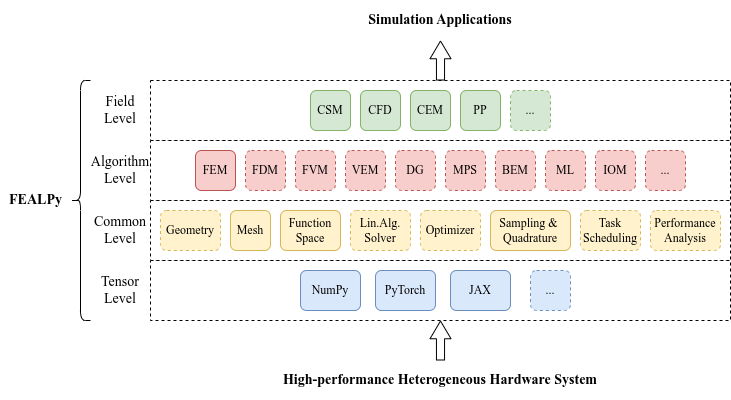
\includegraphics[width=0.8\textwidth]{figures/fealpy_structure.png}
	\caption{The layered architecture of FEALPy, comprising tensor, common, algorithm, and field levels, progressing from low-level functionalities to high-level applications. Modules in dashed boxes are under development.}
	\label{fs:fig1}
\end{figure}

Specifically, the functions of each layer are as follows:
\begin{itemize} 
	\item \textbf{Tensor level}: Provides basic tensor operations and manages backend systems such as NumPy, PyTorch, and JAX through the \textit{Tensor Backend Manager}. This mechanism forms the foundation for SOPTX's multi-backend switching. In particular, the automatic differentiation (AD) features of PyTorch and JAX enable automatic computation of sensitivities for objective and constraint functions in topology optimization (TO), greatly simplifying the derivative evaluation process.
	\item \textbf{Common level}: Includes components such as mesh generation and finite element spaces, offering the capability to rapidly construct meshes and function spaces required for finite element analysis in TO. This serves as the foundational support for finite element analysis in SOPTX.
	\item \textbf{Algorithm level}: Encompasses solvers and optimization algorithms, providing efficient computational support for optimization methods in SOPTX and ensuring both performance and stability during the optimization process.
	\item \textbf{Field level}: Targets specific physical problems (e.g., linear elasticity), enabling SOPTX to flexibly handle various types of TO problems such as compliance minimization under volume constraints, and offers customized support for application-specific scenarios.
\end{itemize}

Through this layered design, FEALPy balances functionality, extensibility, and performance. In particular, the introduction of the \textit{Tensor Backend Manager} allows users to focus on upper-level algorithms and application logic without worrying about differences in underlying hardware or computational libraries. Moreover, the modules marked as under development in Figure~\ref{fs_fig1} demonstrate FEALPy’s potential for continuous improvement, and the completion of these modules in the future is expected to further enhance SOPTX’s capabilities in solving complex TO problems.

\subsection{SOPTX Architecture Design}
The SOPTX framework is positioned within the field level of FEALPy’s layered architecture, targeting structural topology optimization (STO) applications. SOPTX fully inherits and extends FEALPy’s \textit{Tensor Backend Manager}, diverse numerical algorithm components, and general-purpose mesh and geometry handling capabilities. This design not only ensures flexibility and extensibility, but also significantly improves computational efficiency for TO problems.

As shown in Figure~\ref{fs:fig2}, SOPTX adopts a modular architecture consisting of four primary components: the material, solver, filter, and optimizer modules. These components communicate and share data through well-defined interfaces, forming a loosely coupled and easily extensible multi-backend framework for TO.
% [H] [htp]
\begin{figure}[htp]
	\centering
	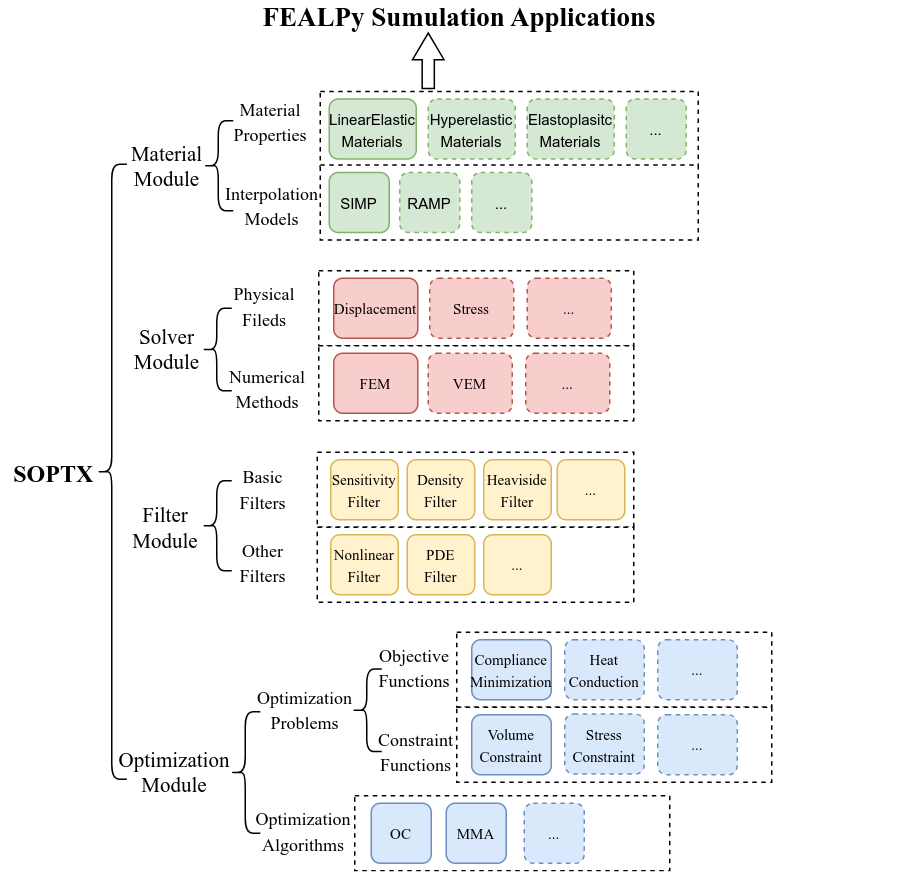
\includegraphics[width=0.8\textwidth]{figures/soptx_structure.png}
	\caption{SOPTX is organized into four main modules: material, solver, filter, and optimization—forming a modular and extensible architecture. The material module provides the foundation, while the solver and filter modules handle intermediate computations and jointly support the optimization module. Dashed boxes indicate components under development.}
	\label{fs:fig2}
\end{figure}

\subsubsection{Material Module}
In its current version, SOPTX primarily focuses on linear elastic materials. The linear elastic material class is developed based on FEALPy’s corresponding implementation and extends its core functionalities---including the computation of Lamé constants, elasticity matrices, and strain matrices---by introducing additional interfaces tailored for TO. At present, the material module implements the Solid Isotropic Material with Penalization (SIMP) interpolation model, typically using a penalization factor $p = 3$, which effectively transforms continuously varying density fields into discrete material distributions. The module is designed with highly abstract interfaces, ensuring extensibility. This design allows for easy future extensions to support other interpolation models such as the Rational Approximation of Material Properties (RAMP), as well as more complex material behaviors, including anisotropic, hyperelastic, and elastoplastic materials. These extensions can be realized by subclassing the base material class and implementing the required interfaces, without modifying other parts of the framework.

The material module encapsulates the interpolation, update, and evaluation of elastic constants within a unified interface, enabling convenient access to material information for downstream modules. Its main functional interfaces include:
\begin{enumerate}
	\item Computing elasticity tensors from a given density field, providing material stiffness data required by the solver module.
	\item Supporting efficient batch updates of material properties, suitable for repeated evaluations in iterative optimization processes.
	\item Supplying essential material parameters for the optimization module, such as the elastic constants of the base material.
\end{enumerate}
These interfaces maintain a consistent calling convention across different computational backends, while their internal implementations are optimized according to backend-specific characteristics to ensure maximal computational efficiency. With this design, the material module serves as a key component in SOPTX, bridging physical modeling and numerical optimization. It maintains functional independence while providing essential material information throughout the topology optimization workflow. The modular structure not only simplifies the solution of current linear elasticity problems, but also offers a flexible foundation for future extensions to more complex material models.

\subsubsection{Solver Module}
The solver module serves as the computational core of the SOPTX framework. It is responsible for formulating and solving physical field problems (e.g., displacement fields) given material properties, boundary conditions, and external loads. The key design principle of this module is to construct an efficient, flexible, and backend-independent solver engine that meets the demands of repeatedly solving large-scale linear systems in TO. During iterative optimization, solving the physical field often becomes the main performance bottleneck as the design variables are updated. To address this, the solver module emphasizes computational efficiency through optimized matrix assembly, intelligent caching strategies, and multi-backend acceleration. It achieves high performance across various computational backends (NumPy / PyTorch / JAX). Meanwhile, the module maintains loose coupling with other components by accessing material data and providing results through clearly defined interfaces, ensuring smooth backend switching and modular extensibility.

In the current version, SOPTX primarily focuses on solving linear elasticity equations using the finite element method (FEM). The FEM solver class is developed based on FEALPy's finite element module, inheriting core functionalities such as linear elasticity integrators and finite element computation components. The solver module implements several key features:
\begin{enumerate}
	\item \textbf{Dimensional and element adaptability}: It supports various spatial dimensions, element types, and boundary condition formulations, accommodating diverse engineering analysis requirements. In the current version, given that the density field is represented as piecewise constant per element, the displacement field is discretized using linear finite elements to ensure numerical stability and computational efficiency.
	\item \textbf{Efficient numerical strategies}: In addition to standard finite element integration and matrix assembly, a fast matrix assembly technique is implemented. This approach separates the element-independent and element-dependent parts of the stiffness matrix, avoiding redundant computations common in traditional methods and significantly improving efficiency for large-scale problems. Furthermore, symbolic integration is supported, enabling pre-computed exact expressions without the need for numerical quadrature, thereby further reducing computational cost.
	\item \textbf{Multiple solution strategies}: The module supports both direct solvers (e.g., MUMPS) and iterative solvers (e.g., Conjugate Gradient, CG), allowing users to select the most suitable algorithm based on problem size and characteristics. Solver strategies are automatically optimized for the underlying backend—for example, leveraging GPUs acceleration for large sparse matrix computations on PyTorch and JAX backends. 
\end{enumerate}

The solver module is designed with strong extensibility. In terms of physical fields, beyond the current displacement field solver, the framework is planned to support efficient computation of additional fields such as stress. Regarding numerical methods, SOPTX intends to extend beyond the classical FEM to incorporate advanced techniques such as the Virtual Element Method (VEM). Moreover, the framework is extensible to accommodate nonlinear mechanics problems, multiphysics coupling, adaptive mesh refinement strategies, and parallel computing. In particular, as the framework evolves toward multi-resolution topology optimization, it will support intra-element heterogeneous density distributions and corresponding high-order finite element displacement fields, thereby improving both boundary resolution and optimization quality. All these extensions can be realized by extending the base solver class or introducing specialized solvers, without altering the overall architecture of the framework.

The solver module plays a pivotal role in SOPTX by bridging physical analysis and optimization computation. Its interactions and responsibilities are summarized as follows:
\begin{enumerate}
	\item \textbf{Interaction with the material module}: The solver module receives material properties such as elasticity matrices from the material module, which are used to assemble the global stiffness matrix. This interaction is handled via unified interfaces, so that the solver does not depend on the specific material interpolation scheme.
	\item \textbf{Output to the optimization module}: The solver module provides two key types of outputs to the optimization module: the displacement field, which is used to evaluate the objective function, and the stiffness matrix, which is used in sensitivity analysis. These outputs follow consistent interface definitions across different backends, while their internal representations are backend-specific and optimized to ensure efficient downstream computations.
	\item \textbf{Result reuse}: Given the iterative nature of topology optimization, the solver module incorporates an intelligent caching mechanism to avoid redundant computations of invariant components (e.g., shape function derivative matrices). This significantly reduces computational overhead, particularly in large-scale problems.
\end{enumerate}
Through its modular design and clearly defined interfaces, the solver module performs physical field computations efficiently, providing essential computational support for the entire topology optimization process while maintaining consistency and high performance across multi-backend environments.

\subsubsection{Filter Module}
The filter module is a key component in SOPTX responsible for processing design variables and applying regularization. It plays a dual role in the topology optimization process: eliminating numerical instabilities such as checkerboarding and mesh dependency, and enhancing the manufacturability of the resulting structures. Following the overall loosely coupled design philosophy of the framework, the filter operations are implemented as an independent functional unit, while maintaining efficient data exchange with other modules. Similar to the material and solver modules, the filter module provides a consistent interface across different computational backends (NumPy / PyTorch / JAX), while its internal implementations are optimized according to backend-specific features to ensure maximal computational efficiency.

In the current version of the SOPTX framework, the filter module implements three main types of filtering techniques:
\begin{enumerate}
	\item \textbf{Sensitivity filtering}: Applies weighted averaging to the sensitivities of the objective function, effectively suppressing checkerboard patterns.
	\item \textbf{Density filtering}: Directly filters the design variables by mapping raw design values to physical densities, addressing the locality issues that may arise with sensitivity filtering in some problems.
	\item \textbf{Heaviside projection filtering}: Builds upon density filtering by applying a smoothed Heaviside function to force intermediate densities toward $0$ or $1$, thereby promoting clear black-and-white structural designs.
\end{enumerate}

The filter module constructs its filtering matrices using a KD-tree-based neighborhood search algorithm. Traditional linearly decaying filters are typically restricted to structured grids, but by leveraging the KD-tree data structure, SOPTX enables efficient spatial queries for neighboring points. This allows filtering to be seamlessly applied to arbitrary unstructured meshes and complex geometries, greatly expanding the applicability of the framework. To further enhance computational performance, the module adopts several optimization strategies, including precomputation of filter neighborhoods, sparse matrix representations, and backend-specific adaptations. These strategies ensure that filtering operations remain efficient even in large-scale topology optimization problems.

The filter module is designed with strong extensibility. Users can easily incorporate new filtering algorithms by subclassing the base filter class and implementing the required interfaces. Examples include nonlinear filters, PDE-based filters with exponential decay kernels, or filters based on alternative kernel functions. These newly added filters automatically inherit multi-backend compatibility without requiring additional adaptation. Moreover, the SOPTX framework supports chained composition of filters. Users can flexibly configure and combine multiple basic filters to construct complex filtering strategies that meet the specific requirements of different optimization scenarios.

The interactions between the filter module and other components are as follows:
\begin{enumerate}
	\item \textbf{Interaction with the solver module}: It receives the raw design variables and outputs the filtered physical density field.
	\item \textbf{Interaction with the optimizer module}: It takes in the unfiltered sensitivities computed by the optimization algorithm and returns the filtered sensitivities, ensuring numerical stability during the optimization process.
	\item \textbf{Coordination with the material module}: The filtered physical density is directly used for material interpolation, forming a clear data flow:
	\begin{equation*}
		\text{design variables} \to \text{filtering} \to \text{physical density} \to \text{material properties} \to \text{physical response}.
	\end{equation*}
\end{enumerate}
Through this modular design, the filter module effectively addresses numerical instability issues in TO and offers a flexible mechanism for extending various regularization strategies. Within the SOPTX framework, the filter module is not only an essential part of the optimization workflow but also a key enabler for achieving high-quality and manufacturable structural designs.

\subsubsection{Optimization Module}
The optimization module serves as the computational core of the SOPTX framework, responsible for integrating physical field solutions with optimization objectives to formulate complete mathematical optimization problems and invoke corresponding algorithms for their solution. Closely interacting with the material, solver, and filter modules, it completes the full computational pipeline for TO. Like other modules, the optimization module follows the multi-backend design philosophy of the framework, providing a consistent interface across NumPy, PyTorch, and JAX backends. Its internal implementations are backend-optimized to ensure high performance on each platform.

In the current version, the optimization module focuses on the classical compliance minimization problem under volume constraints and supports two mainstream topology optimization algorithms: Optimality Criteria (OC) and the Method of Moving Asymptotes (MMA). The MMA implementation is based on the standard version proposed by Svanberg in 2007\cite{Svanberg2007MmaAG}, and has been extended in SOPTX to support multiple backend implementations. While preserving mathematical equivalence, backend-specific optimizations have been introduced to improve computational performance, particularly enabling GPUs acceleration in PyTorch and JAX environments.

The design of the optimization module follows two core principles:
\begin{enumerate}
	\item \textbf{Separation of problem definition and algorithm}: The definition of the optimization problem---namely, the objective functions, the constraint functions, and their sensitivities---is strictly decoupled from the optimization algorithms. This allows users to flexibly combine different problem formulations with various optimization solvers.
	\item \textbf{Dual-mode sensitivity computation}: The framework supports both manually derived and automatically differentiated sensitivities. On PyTorch and JAX backends, users can directly leverage AD to avoid complex manual derivations, while still preserving the physical consistency and interpretability offered by hand-derived formulations.
\end{enumerate}

The optimization module is designed with high extensibility:
\begin{enumerate}
	\item \textbf{Problem type extension}: Users can easily define new optimization objectives---such as heat conduction, Compliant mechanism synthesis, or multiphysics problems---and corresponding constraint conditions, such as stress or frequency constraints, by subclassing the base optimization problem class.
	\item \textbf{Algorithm extensibility}: The framework allows integration of new optimization algorithms, including Sequential Quadratic Programming (SQP), Sequential Linear Programming (SLP), and other gradient-based methods.
\end{enumerate}

The optimization module serves as a central hub within the SOPTX framework, coordinating closely with other modules through the following interactions:
\begin{enumerate}
	\item \textbf{Interaction with the solver module}: It receives physical field outputs such as the displacement field and stiffness matrix, which are used to evaluate the objective function (e.g., compliance) and its corresponding sensitivities.
	\item \textbf{Interaction with the filter module}: It passes raw sensitivities to the filter module for processing and receives the filtered sensitivities to update the design variables. Additionally, the newly updated design variables are filtered again to obtain the physical density field.
\end{enumerate}

Through this modular and flexible design, the optimization module not only efficiently solves the classical TO problems supported in the current version, but also lays a solid foundation for future extensions to more complex optimization scenarios. As the decision-making center of the SOPTX framework, it integrates the computational capabilities of all other modules into a complete structural design solution.

\subsection{Multi-Backend Switching}
In the field of STO, improving computational performance has always been a central concern in both research and engineering applications. To effectively address the diverse computational demands of problems at different scales, the SOPTX framework builds upon FEALPy to implement a flexible multi-backend support architecture. This allows users to seamlessly switch between multiple tensor computation backends such as NumPy, PyTorch, and JAX. This design not only enhances the applicability and efficiency of the software but also improves its portability and flexibility across different hardware and software platforms. 

Specifically, different computational backends offer distinct advantages and are suitable for different application scenarios: 
\begin{itemize} 
	\item \textbf{NumPy backend}: Suitable for small-scale computational tasks and rapid prototyping. It offers stable performance and broad community support. Due to its lightweight nature and efficient memory management, it is particularly well-suited for fast development and algorithm validation on standard CPUs platforms.
	\item \textbf{PyTorch and JAX backends}: Both support GPUs acceleration and AD, making them ideal for large-scale or high-dimensional problems. The AD capability greatly simplifies the computation of sensitivities for objective and constraint functions, improving development efficiency and significantly shortening the research cycle. JAX goes one step further by offering more flexible compilation strategies and automatic vectorization, achieving high computational efficiency, especially on GPUs platforms.
\end{itemize}

\section{Getting Started with SOPTX}
This chapter aims to provide readers with installation instructions and usage guidance for SOPTX, helping them quickly become familiar with the basic operations of the framework and apply it to topology optimization (TO) tasks. As a TO toolkit built on top of FEALPy, SOPTX offers a highly efficient and flexible computational environment through its multi-backend switching mechanism and modular design. The content of this chapter is divided into two parts: first, we present a detailed explanation of the installation steps for SOPTX and its dependency FEALPy, ensuring that readers can correctly configure the development environment; then, we demonstrate the usage workflow of SOPTX through a classical 2D cantilever beam compliance minimization example.

\subsection{Software Installation}
SOPTX is a TO toolkit built on top of FEALPy, an intelligent CAE simulation engine that provides numerical computing capabilities. Installing FEALPy is a prerequisite, and it is recommended to install it from source. Before installation, ensure that Git and Python are properly installed. It is also recommended to use a virtual environment when installing and running FEALPy.
 
Core installation steps:
\begin{enumerate} 
	\item Clone the FEALPy repository from GitHub:
\begin{lstlisting}[language=bash]
	git clone https://github.com/weihuayi/fealpy.git
\end{lstlisting}
	\item Change into the FEALPy directory and install it in editable mode:
\begin{lstlisting}[language=bash]
	cd fealpy
	pip install -e . 
\end{lstlisting}
	\item Similarly, install SOPTX:
\begin{lstlisting}[language=bash]
	git clone https://github.com:weihuayi/soptx.git
	cd soptx
	pip install -e . 
\end{lstlisting}
\end{enumerate}

For the complete installation guide, please refer to the official documentation at: \url{https://github.com/weihuayi/fealpy}.

\subsection{Example: 2D Cantilever Beam}\label{sec:exp_canti_beam}
We use a popular compliance minimization benchmark to demonstrate the usage of SOPTX \cite{bendsoe2013topology}: minimizing the structural compliance of a cantilever beam under tip loading (see Figure~\ref{fig:cantilever}). The left end of the beam is fixed, and a downward concentrated load $T = -1$ is applied to the bottom of the right end. A $160 \times 100$ uniform quadrilateral mesh is used. The target volume fraction is set to $0.4$, with material properties $E = 1$ and $\nu = 0.3$. The penalization factor is $p = 3$, and the sensitivity filter radius is $r = 6.0$, which matches the mesh element size to ensure structural smoothness and eliminate checkerboard patterns.
\begin{figure}[htp]
	\centering
	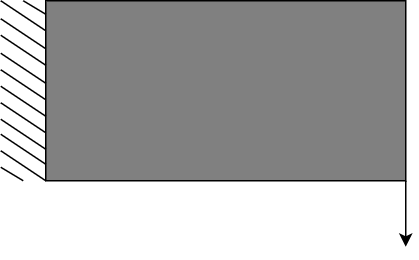
\includegraphics[width=0.6\textwidth]{figures/cantilever_2d.png}
	\caption{Cantilever beam geometry: fixed on the left, with a downward concentrated load on the right.}
	\label{fig:cantilever}
\end{figure}

As shown in Code~\ref{code:mouldes_pde}, we first import relevant modules from FEALPy---including the backend, mesh, and function space---and from SOPTX, including the material, solver, filter, and optimization modules. Next, we define the partial differential equation (PDE) model of the cantilever beam, which includes the geometric configuration, applied load, and boundary conditions. The standard interface of a PDE model in SOPTX includes initialization, region definition, loading, and boundary conditions. The complete definition of the cantilever beam model \texttt{Cantilever2dData1} is provided in~\ref{sec:code_canti_2d}
\begin{lstlisting}[caption={Module imports and PDE model}, label={code:mouldes_pde}]
	from fealpy.backend import backend_manager as bm
	from fealpy.mesh import UniformMesh2d
	from fealpy.functionspace import LagrangeFESpace, TensorFunctionSpace
	
	from soptx.material import (DensityBasedMaterialConfig, DensityBasedMaterialInstance)
	from soptx.solver import (ElasticFEMSolver, AssemblyMethod)
	from soptx.filter_ import SensitivityBasicFilter
	from soptx.opt import (ComplianceObjective, ComplianceConfig, VolumeConstraint, VolumeConfig)
	from soptx.opt import OCOptimizer
	
	from soptx.pde import Cantilever2dData1
	
	pde = Cantilever2dData1(xmin=0, xmax=160, ymin=0, ymax=100,	T = -1)
\end{lstlisting}

As shown in Code~\ref{code:mesh_space}, the mesh and finite element function spaces are defined. The displacement field is represented using the first-order continuous Lagrange space, while the density field is defined in the zeroth-order discontinuous Lagrange space.
\begin{lstlisting}[caption={Mesh and function space definitions}, label={code:mesh_space}]
	mesh = UniformMesh2d(extent=[0, 160, 0, 100], h=[1, 1], origin=[0, 0])
	
	space_C = LagrangeFESpace(mesh=mesh, p=1, ctype='C')
	tensor_space_C = TensorFunctionSpace(scalar_space=space_C, shape=(-1, 2))
	space_D = LagrangeFESpace(mesh=mesh, p=0, ctype='D')
\end{lstlisting}

As shown in Code~\ref{code:material}, the material module is instantiated using the material properties, the SIMP interpolation model, and the TO constants.

\begin{lstlisting}[caption={Material module}, label={code:material}]
	material_config = DensityBasedMaterialConfig(
	elastic_modulus=1.0,            
	minimal_modulus=1e-9,         
	poisson_ratio=0.3,            
	plane_assumption="plane_stress",    
	interpolation_model="SIMP",    
	penalty_factor=3.0)
	materials = DensityBasedMaterialInstance(config=material_config)
\end{lstlisting}
	
As shown in Code~\ref{code:solver_filter}, the solver module is instantiated using the material module, the PDE model, the matrix assembly method, and direct linear system solver (MUMPS). Subsequently, the sensitivity filter is initialized using the specified filter radius.
\begin{lstlisting}[caption={Solver and filter module}, label={code:solver_filter}] 
	solver = ElasticFEMSolver(
					materials=materials,
					tensor_space=tensor_space_C,
					pde=pde,
					assembly_method=AssemblyMethod.STANDARD,
					solver_type='direct',
					solver_params={'solver_type': 'mumps'})
	sens_filter = SensitivityBasicFilter(mesh=mesh, rmin=6.0)
\end{lstlisting}

As shown in Code~\ref{code:optimizer}, the objective function class is instantiated, followed by the volume constraint class based on the specified volume fraction. The optimizer is then initialized using the Optimality Criteria (OC) algorithm with its basic parameters. The maximum number of iterations is set to $200$, and the convergence tolerance is set to $0.01$ to control the termination criteria of the optimization process.

\begin{lstlisting}[caption={Optimization module}, label={code:optimizer}]
	objective = ComplianceObjective(solver=solver)
	constraint = VolumeConstraint(solver=solver, volume_fraction=0.4)
	
	optimizer = OCOptimizer(objective=objective,
	constraint=constraint,
	filter=sens_filter,
	options={'max_iterations': 200, 'tolerance': 0.01})
\end{lstlisting}

As shown in Code~\ref{code:main_post}, the initial density field is defined using an interpolation method. The optimization process is then executed, followed by saving the results and plotting the convergence history.
\begin{lstlisting}[caption={Main program and post-processing}, label={code:main_post}]
	if __name__ == "__main__":
		@cartesian
		def density_func(x):
			val = bm.ones(x.shape[0])
			# val = config.volume_fraction * bm.ones(x.shape[0], **kwargs)
			return val
		rho = space_D.interpolate(u=density_func)
		rho_opt, history = optimizer.optimize(rho=rho[:])
		
		from soptx.opt import save_optimization_history, plot_optimization_history
		save_optimization_history(mesh, history)
		plot_optimization_history(history)
\end{lstlisting}

The initial material density is uniformly distributed across the design domain, with each element initialized to the target volume fraction of $0.4$. After running the code, Figure~\ref{fig:canti_04_convergence} shows the convergence histories of the compliance $c(\rho)$ and the volume fraction $v(\rho)$. The compliance $c(\rho)$ drops rapidly from its initial value of approximately $500$ to around $100$ within the first 10 iterations, and then converges smoothly, reaching convergence at iteration 57. The volume fraction $v(\rho)$ remains stably around $0.4$, with only minor fluctuations.
\begin{figure}[htp]
	\centering
	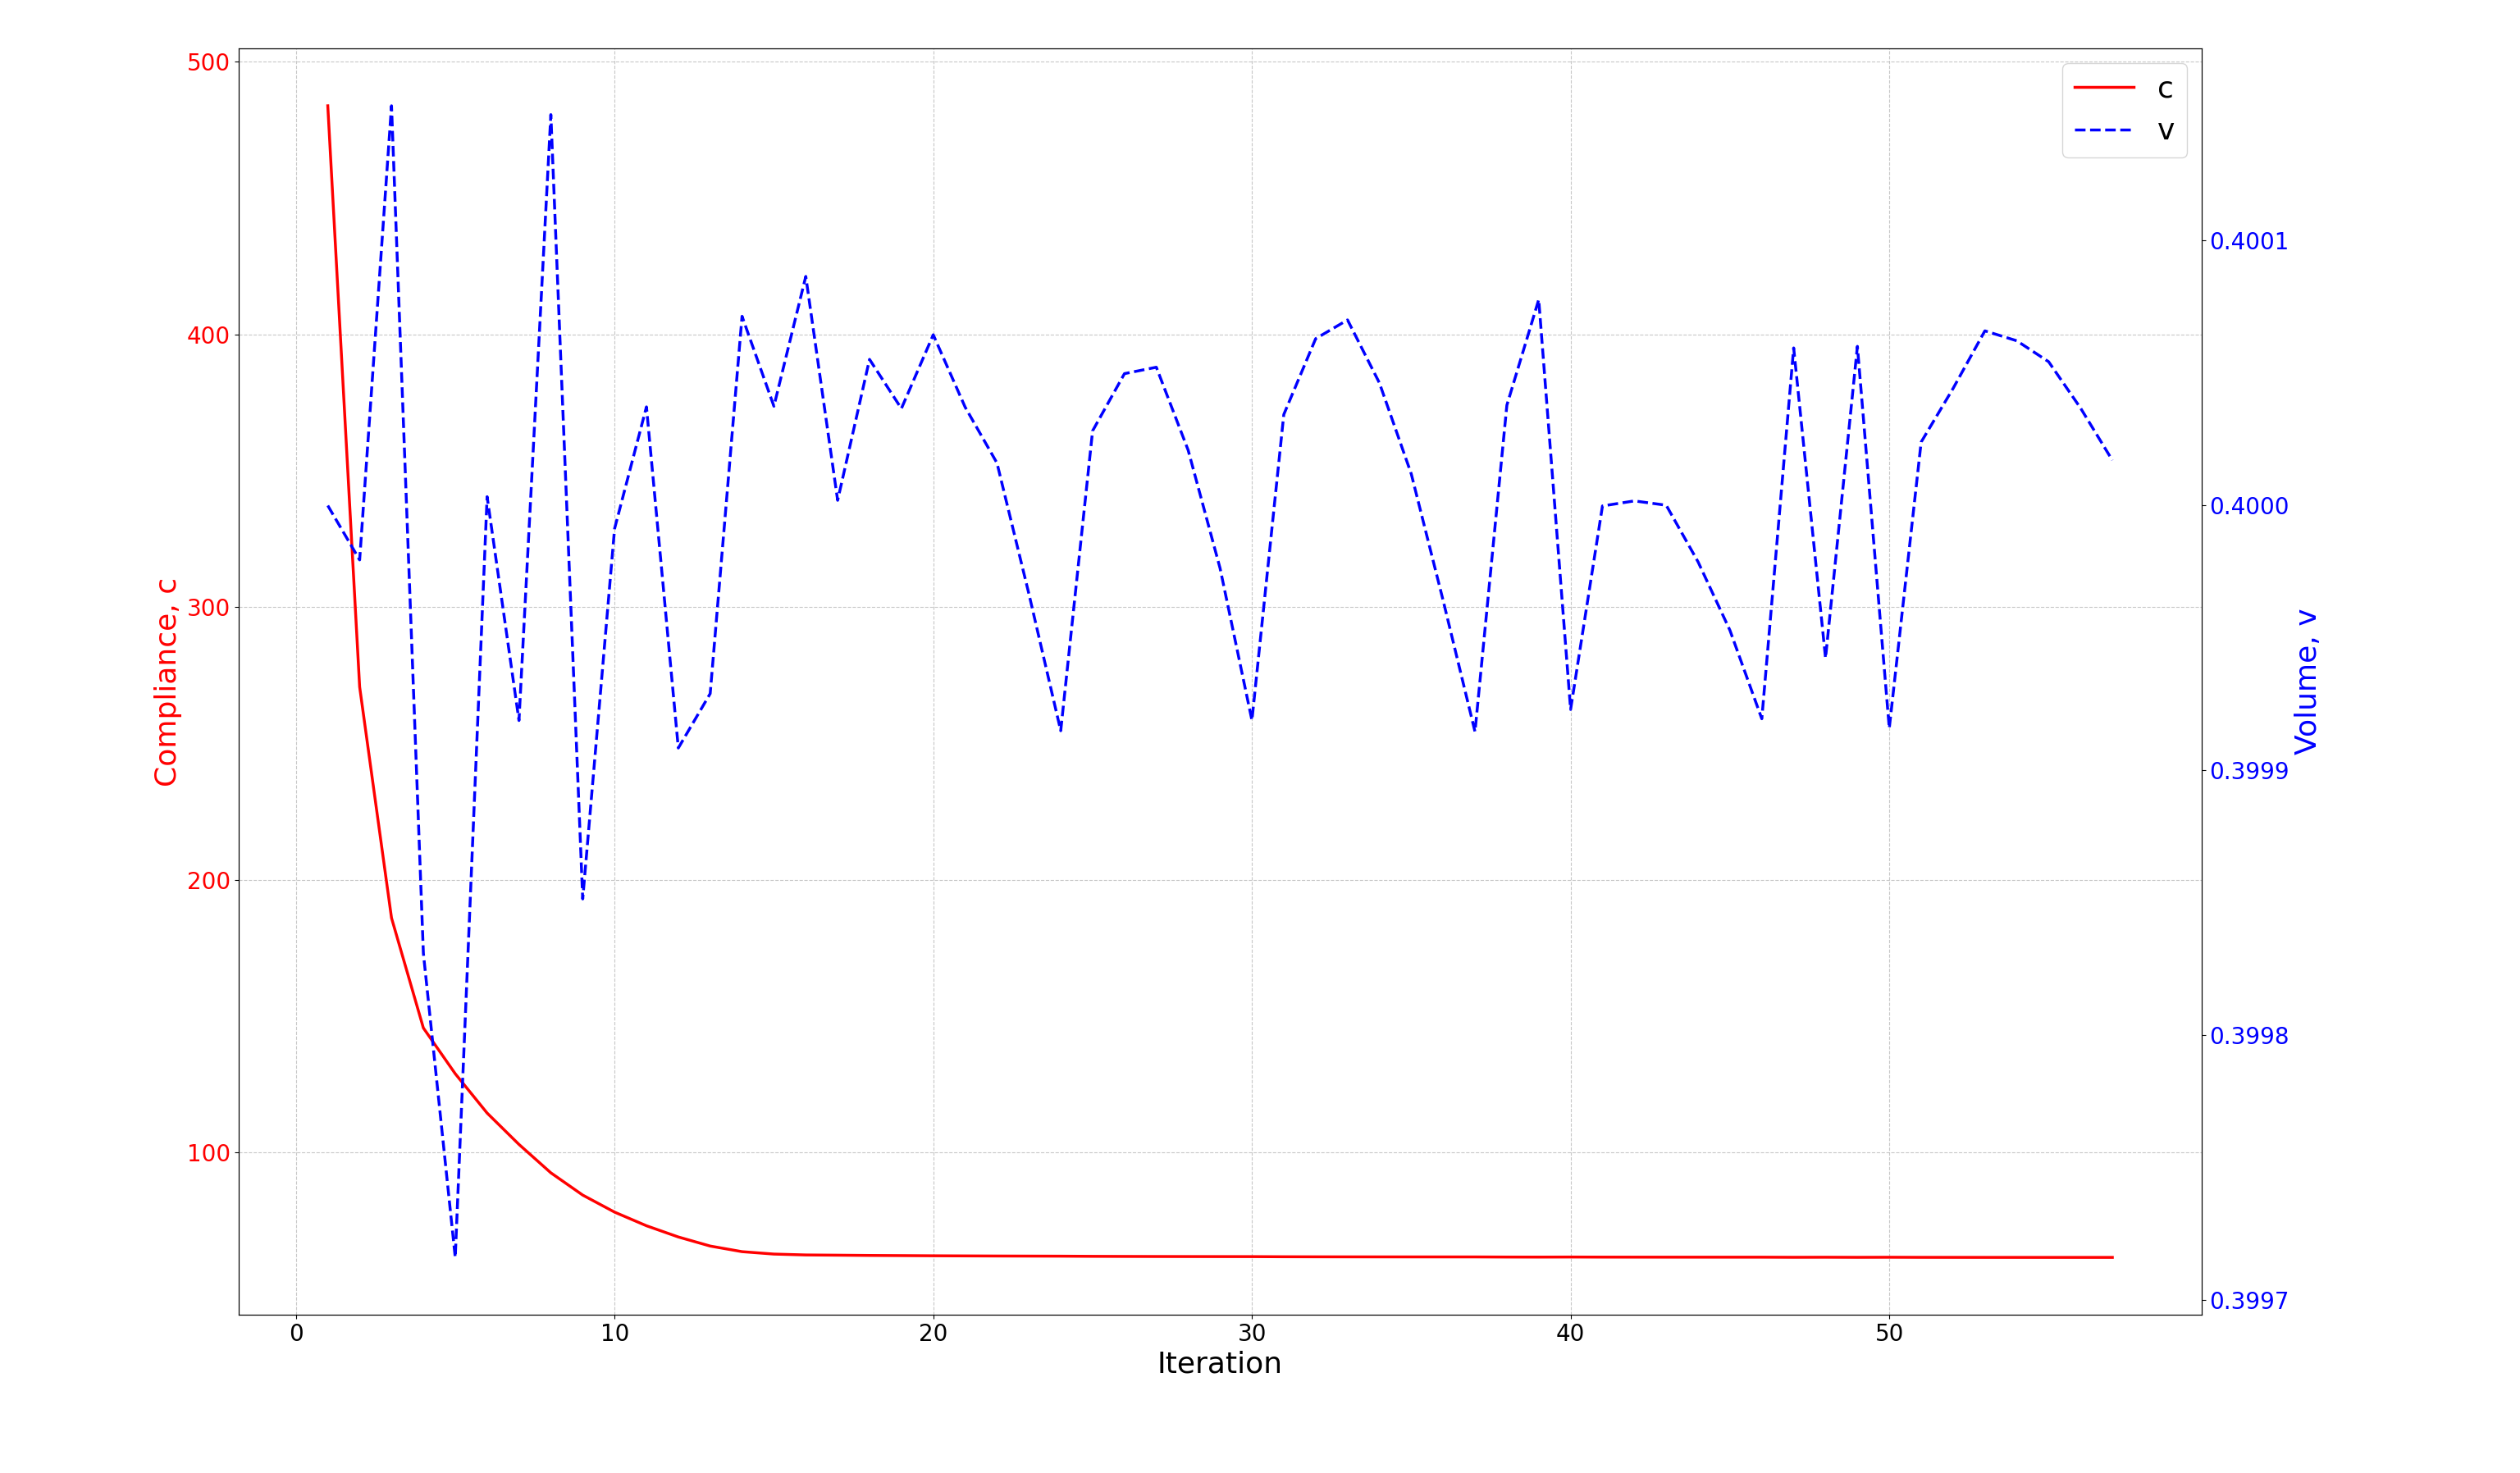
\includegraphics[width=1.0\textwidth]{figures/cantilever_2d_04_convergence.png}
	\caption{Convergence histories of the compliance $c(\rho)$ and volume fraction $v(\rho)$ for the 2D cantilever beam initialized with a uniform density of $0.4$.}
	\label{fig:canti_04_convergence}
\end{figure}

Figure~\ref{fig:canti_04_all} displays the resulting topologies at iterations 3, 30, and 57.

\begin{figure}[htp]
	\centering
	\subfloat[$c(\rho)=145.5753,~v(\rho)=0.3998$]{
		
\includegraphics[width=0.32\textwidth]{figures/cantilever_2d_04_1.png}
		\label{fig:canti_04_1}
	}
	\subfloat[$c(\rho)=61.7084,~v(\rho)=0.3999$]{
		
\includegraphics[width=0.32\textwidth]{figures/cantilever_2d_04_2.png}
		\label{fig:canti_04_2}
	}
	\subfloat[$c(\rho)=61.4208,~v(\rho)=0.4000$]{
		
\includegraphics[width=0.32\textwidth]{figures/cantilever_2d_04_3.png}
		\label{fig:canti_04_3}
	}
	\caption{Topology layouts at iterations 3, 30, and 57 during the optimization process. Each subfigure also reports the corresponding compliance and volume fraction values.}
	\label{fig:canti_04_all}
\end{figure}

The initial material density is uniformly set to $1$ over the design domain. After running the optimization, Figure~\ref{fig:canti_1_convergence} shows the convergence histories of the compliance $c(\rho)$ and the volume fraction $v(\rho)$. The volume fraction smoothly decreases from $1$ to the target value of $0.4$ and stabilizes after approximately 5 iterations. The compliance $c(\rho)$ first increases from around $30$ to $500$ and then gradually decreases, converging at iteration 60. Compared with the case initialized at $\rho = 0.4$, the optimization process starting from a fully solid design ($\rho = 1$) requires slightly more iterations to converge, as it first reduces the volume fraction to satisfy the constraint before refining the topology.
\begin{figure}[htp]
	\centering
	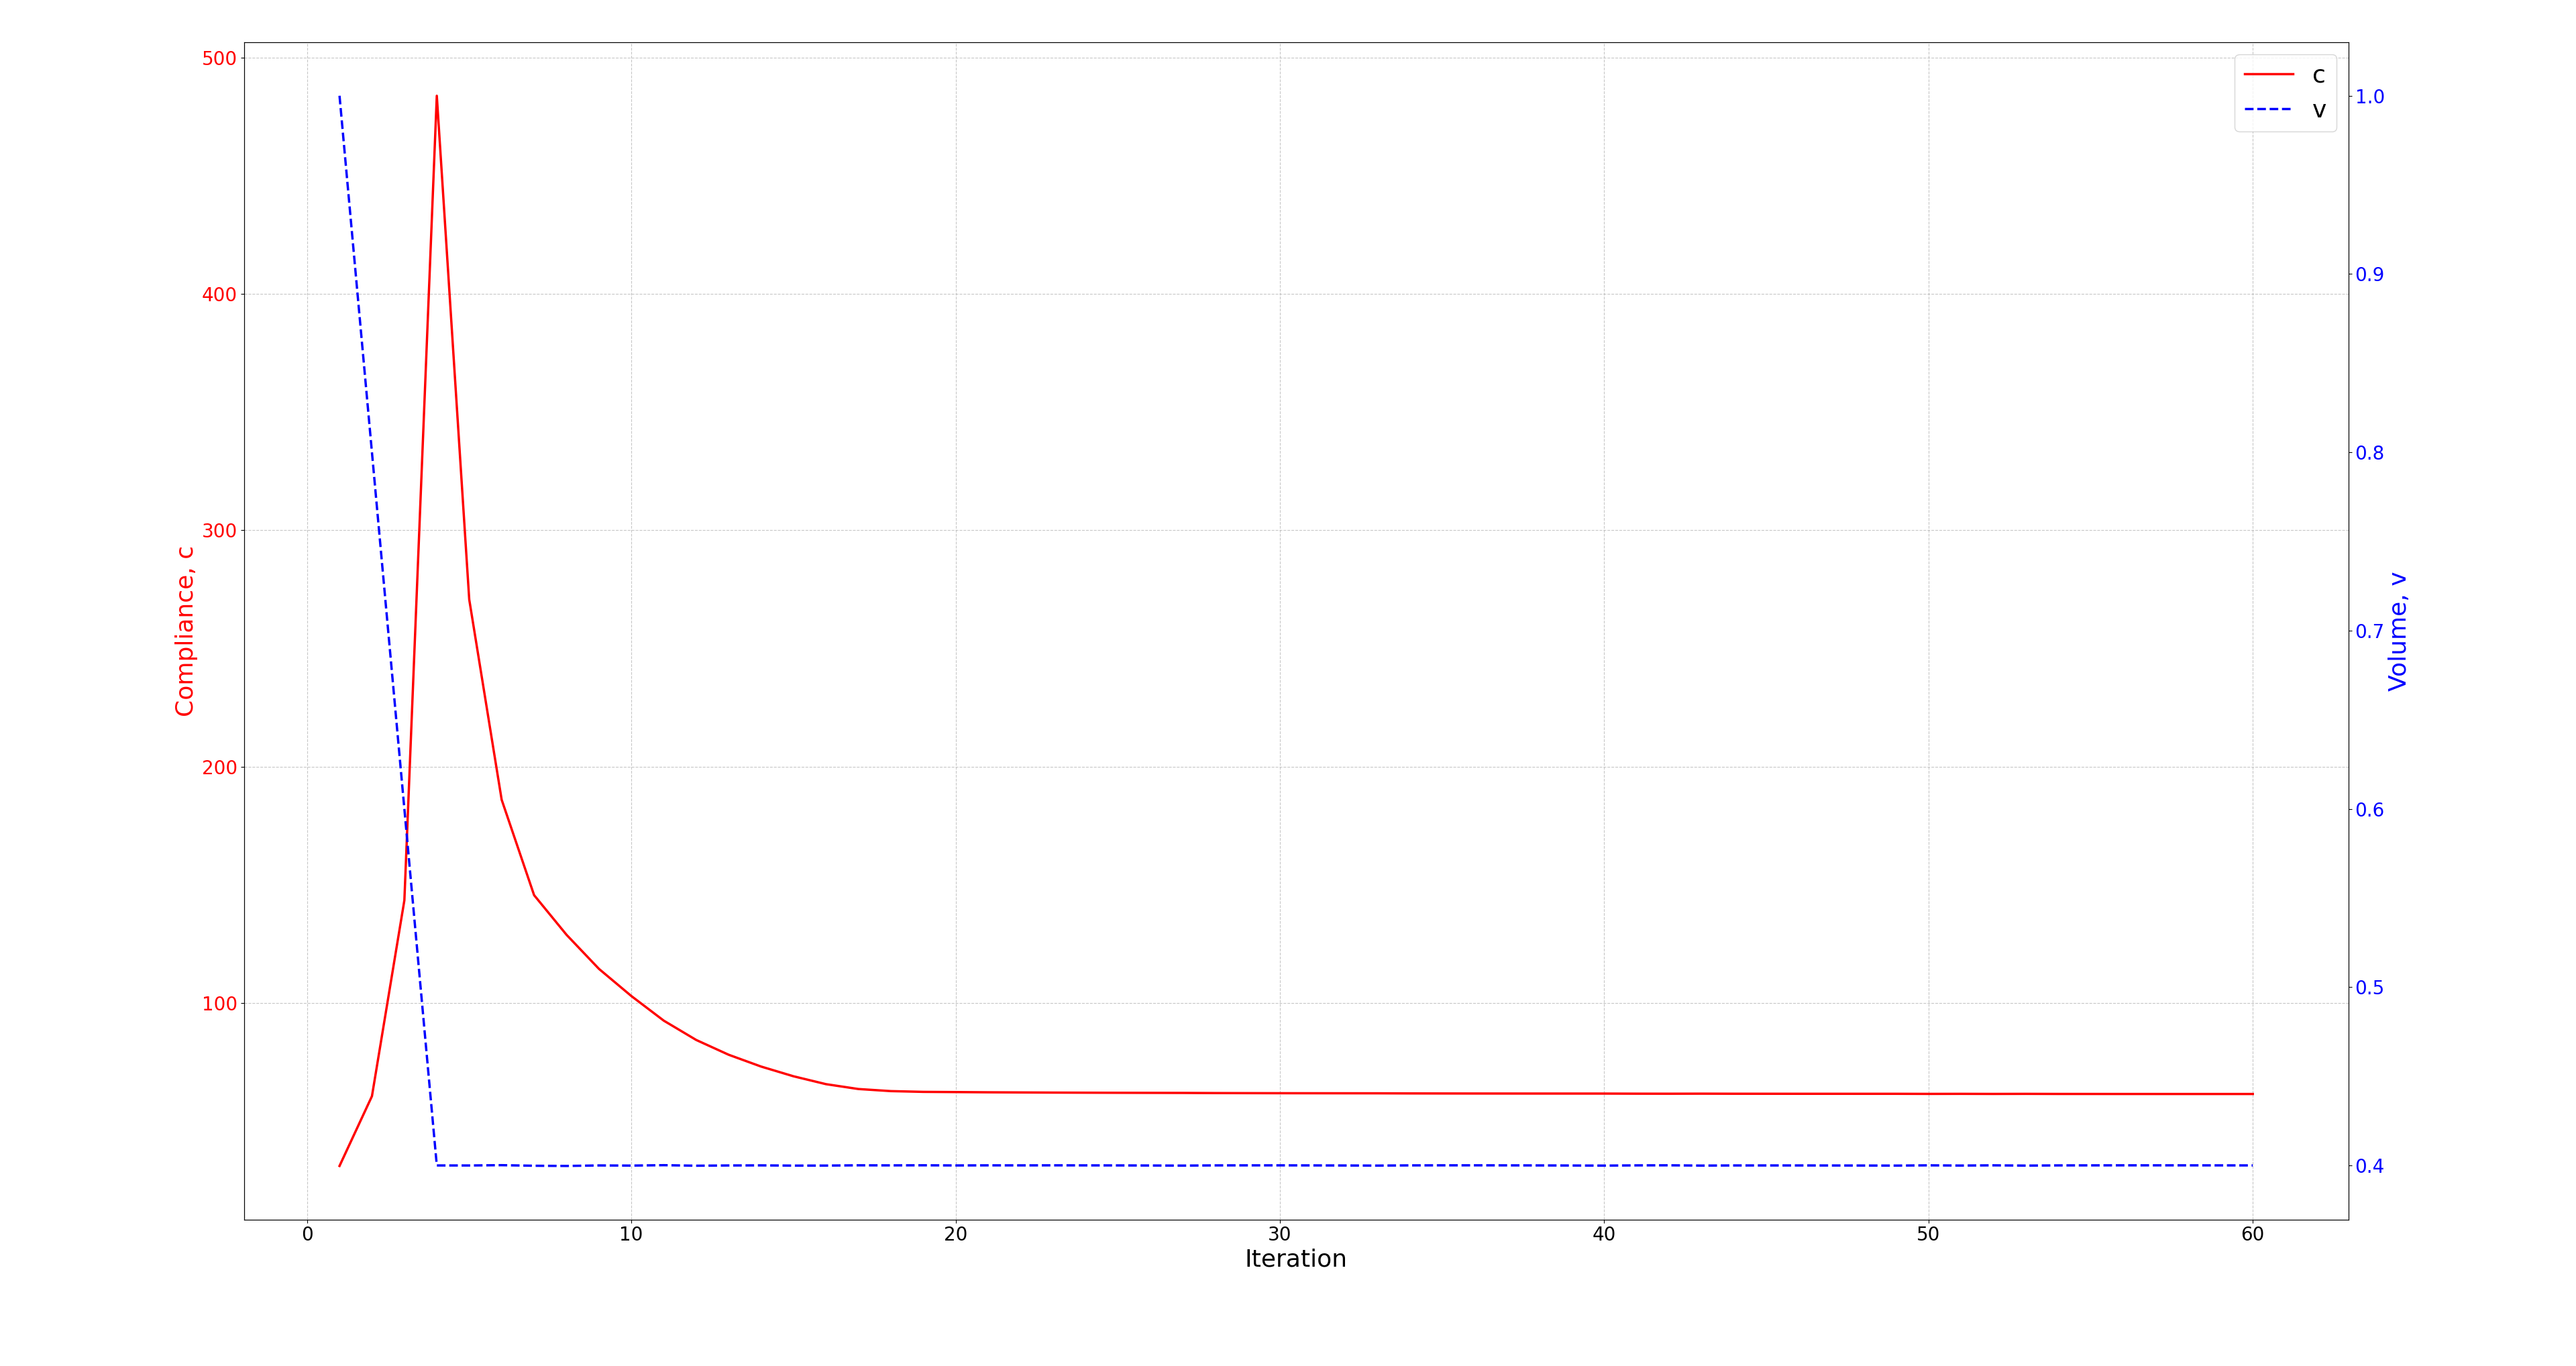
\includegraphics[width=1.0\textwidth]{figures/cantilever_2d_1_convergence.png}
	\caption{Convergence histories of the compliance $c(\rho)$ and volume fraction $v(\rho)$ for the 2D cantilever beam with an initial density of $1$.}
	\label{fig:canti_1_convergence}
\end{figure}

Figure~\ref{fig:canti_1_all} shows the topology layouts at iterations 6, 33, and 60.
\begin{figure}[htp]
	\centering
	\subfloat[$c(\rho)=185.9530,~v(\rho)=0.4002$]{
		
\includegraphics[width=0.32\textwidth]{figures/cantilever_2d_1_1.png}
		\label{fig:canti_1_1}
	}
	\subfloat[$c(\rho)=61.7084,~v(\rho)=0.3999$]{
		
\includegraphics[width=0.32\textwidth]{figures/cantilever_2d_1_2.png}
		\label{fig:canti_1_2}
	}
	\subfloat[$c(\rho)=61.4208,~v(\rho)=0.4000$]{
		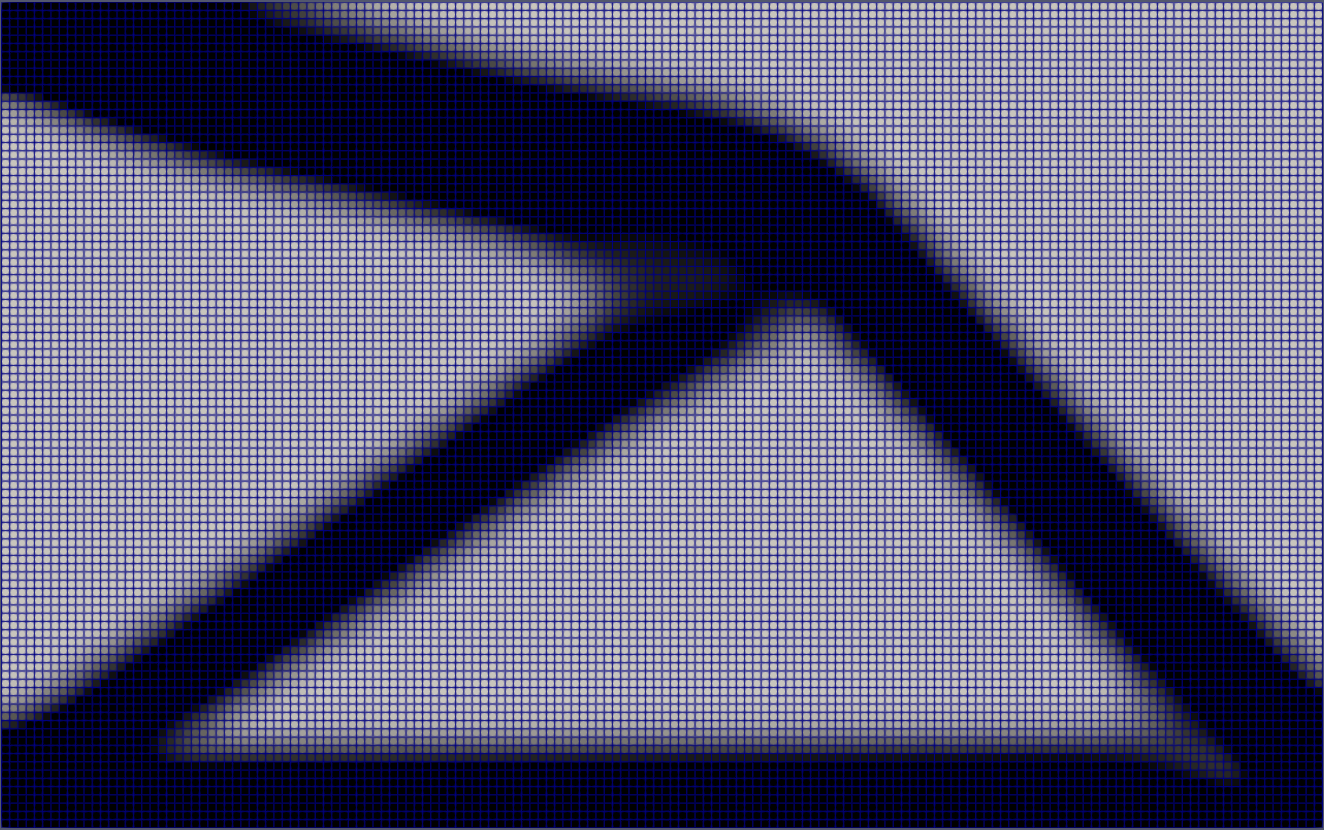
\includegraphics[width=0.32\textwidth]{figures/cantilever_2d_1_3.png}
		\label{fig:canti_1_3}
	}
	\caption{Topology layouts at iterations 6, 33, and 60 during the optimization process. Each subfigure includes the compliance and volume fraction.}
	\label{fig:canti_1_all}
\end{figure}

\section{Numerical Examples}
This chapter presents a series of numerical examples that comprehensively demonstrate the capabilities and performance of the SOPTX framework in topology optimization (TO).  The test cases span from classical 2D Messerschmitt-Bolkow-Blohm (MBB) beam problems to 3D cantilever structures, highlighting the flexibility and robustness of SOPTX in handling different partial differential equation (PDE) models, mesh types, filtering strategies, and optimization algorithms. In addition, this chapter explores the framework’s advanced features, including fast matrix assembly, automatic differentiation (AD), and multi-backend switching, showcasing their significant benefits in improving computational efficiency and simplifying the development workflow.

The chapter is organized into seven sections: first, we present the MBB beam problem to demonstrate the robustness of SOPTX across different mesh resolutions; then, we investigate the impact of different filtering techniques on the optimization results; next, we introduce the algorithm switching interface and a backend-reconstructed version of the MMA optimizer; subsequently, we extend SOPTX to 3D TO; after that, we highlight how fast matrix assembly improves overall runtime efficiency; we then illustrate how AD simplifies the implementation of sensitivity analysis; finally, we discuss the benefits of the multi-backend switching mechanism and demonstrate the GPU acceleration potential. Through these examples, the functionalities of SOPTX are systematically demonstrated, providing readers with guidance for applying the framework in both scientific research and engineering scenarios.

\subsection{MBB Beam}\label{sec:exp_mbb_beam}
The MBB beam is a classical benchmark problem in TO, widely used to verify the effectiveness and robustness of optimization algorithms. In this section, we minimize the structural compliance of the MBB beam (see Figure~\ref{fig:mbb_beam}) to demonstrate the flexibility and consistency of the SOPTX framework in handling different PDE models and mesh settings. The beam is subject to hinged boundary conditions along its left edge and the bottom right corner, where only horizontal displacements are constrained (i.e., zero horizontal movement is enforced while vertical motion is free). A downward concentrated load $T = -1$ is applied to the upper left corner. The target volume fraction is set to $0.5$, and the material parameters are $E = 1$ and $\nu = 0.3$. The penalization factor is $p = 3$, and the filter radius is $r = 6.0$, which matches the mesh element size to ensure smooth topology and suppress checkerboard patterns.
\begin{figure}[htp]
	\centering
	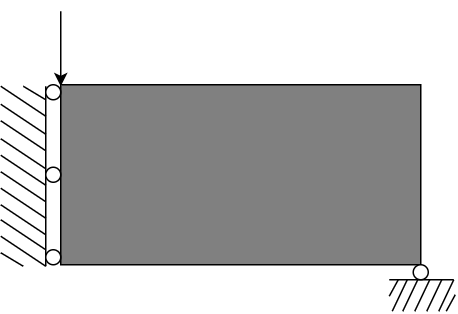
\includegraphics[width=0.8\textwidth]{figures/mbb_2d.png}
	\caption{Geometry of the MBB beam: hinged at the left edge and bottom right corner, with a downward concentrated load applied at the top left.}
	\label{fig:mbb_beam}
\end{figure}

Compared to the cantilever beam example in Section~\ref{sec:exp_canti_beam}, the SOPTX framework allows users to switch to the MBB beam problem with minimal modifications. Thanks to its modular design, it is sufficient to change the PDE model. The full implementation of the MBB beam model \texttt{MBBBeam2dData1} is provided in \ref{sec:code_mbb}
\begin{lstlisting}
	from soptx.pde import MBBBeam2dData1
	pde = MBBBeam2dData1(xmin=0, xmax=150, ymin=0, ymax=50, T = -1)
\end{lstlisting}

To highlight the adaptability and robustness of SOPTX across different mesh types, we perform TO on a $150 \times 50$ uniform quadrilateral mesh and a triangular mesh, both initialized with a uniform material density equal to the target volume fraction $0.5$. The triangular mesh is generated using the following code:
\begin{lstlisting}
	from fealpy.mesh import TriangleMesh
	mesh = TriangleMesh.from_box(box=[0, 150, 0, 50], nx=150, ny=50)
\end{lstlisting}
The resulting topologies are shown in Figure~\ref{fig:mbb_2d_all}:
\begin{figure}[htp]
	\centering
	\subfloat[$c(\rho)=219.5199,~v(\rho)=0.5001$]{
		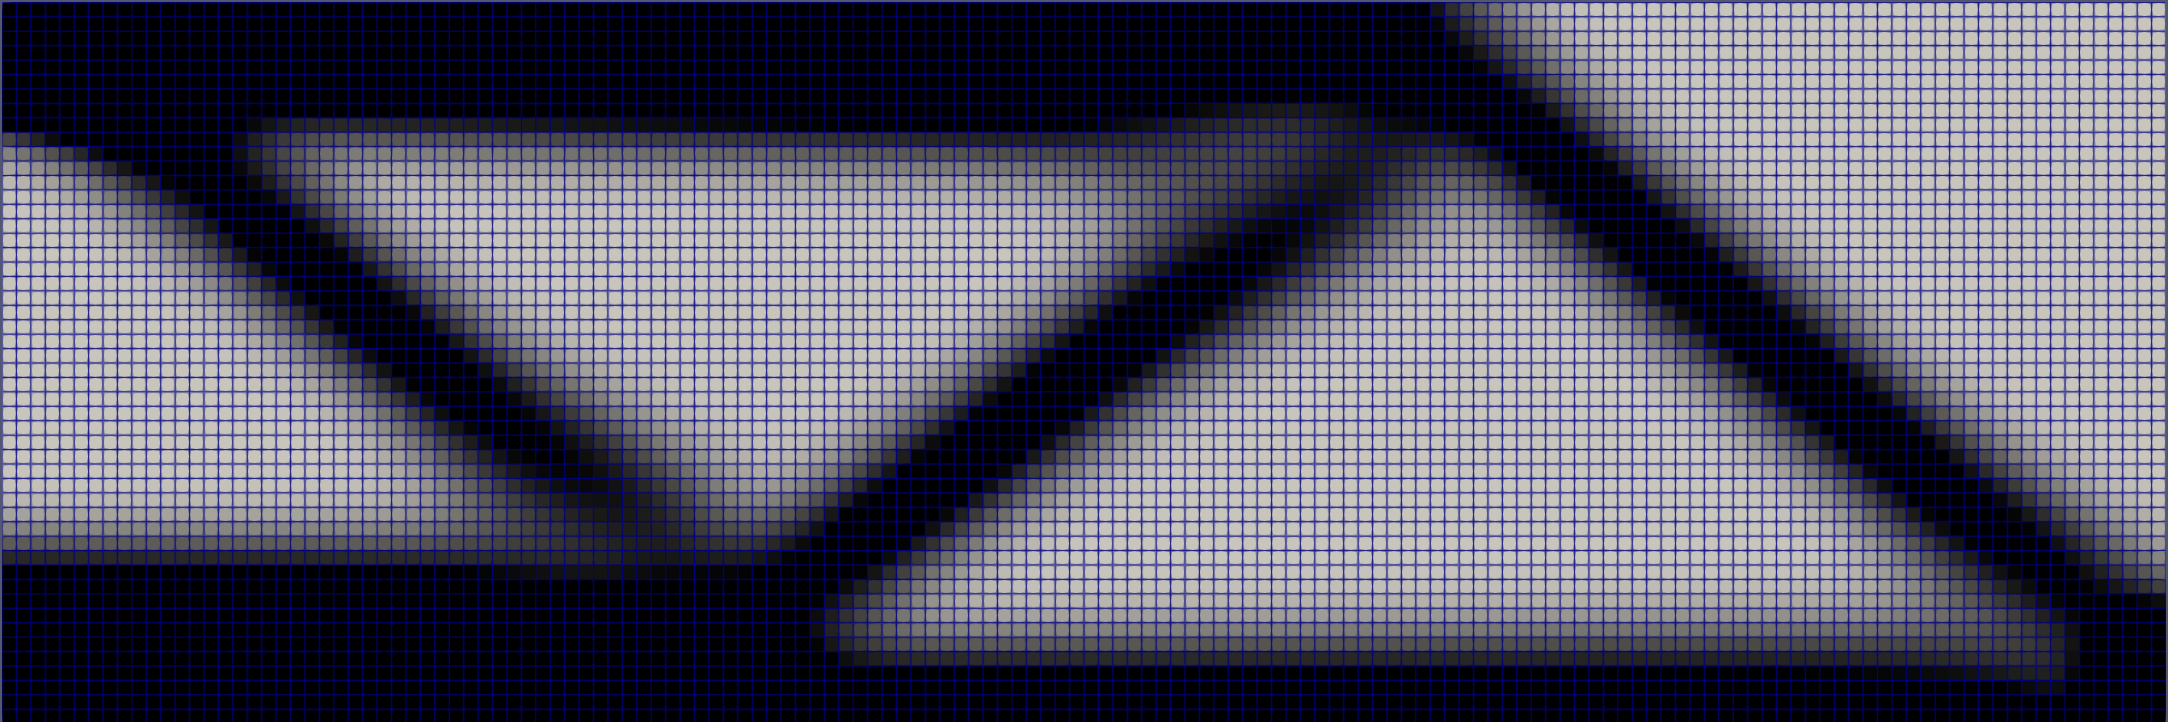
\includegraphics[width=0.5\textwidth]{figures/mbb_2d_u2.png}
		\label{fig:mbb_2d_u2}
	}
	\subfloat[$c(\rho)=217.6605,~v(\rho)=0.4999$]{
		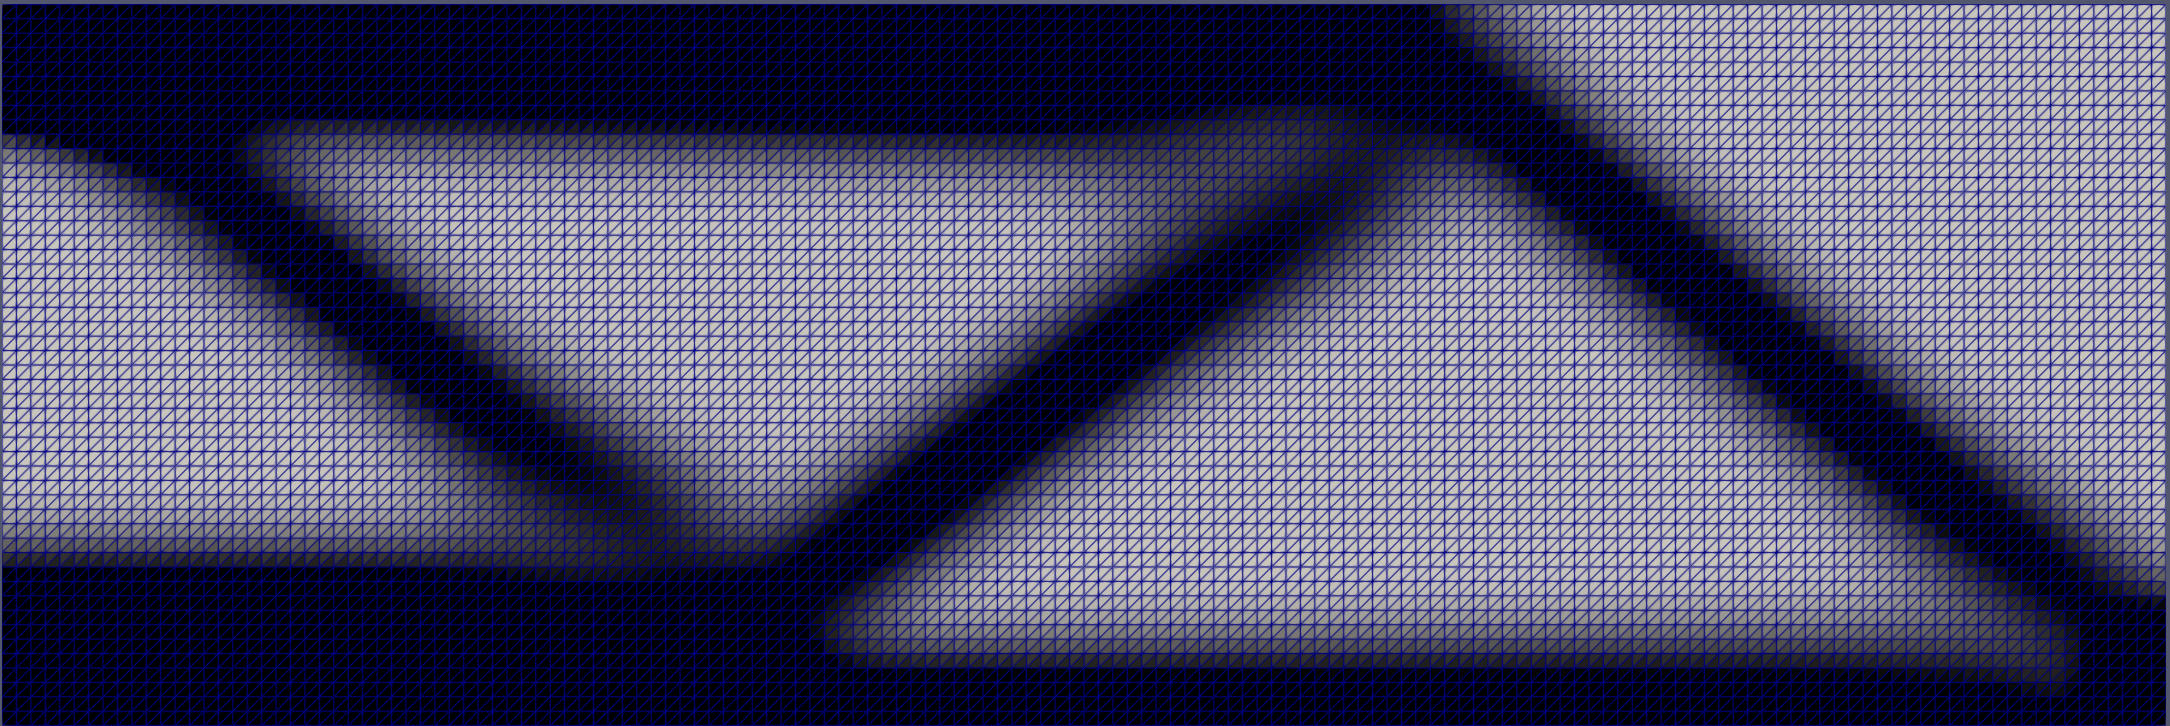
\includegraphics[width=0.5\textwidth]{figures/mbb_2d_tri.png}
		\label{fig:mbb_2d_tri}
	}
	\caption{Optimized topologies of the MBB beam using a uniform quadrilateral mesh (left) and a triangular mesh (right).}
	\label{fig:mbb_2d_all}
\end{figure}

As shown in Figure~\ref{fig:mbb_2d_all}, the optimized layouts under both mesh types are highly consistent, with relative differences in compliance and volume fraction below $1\%$. This consistency demonstrates the mesh-independence and algorithmic robustness of SOPTX. Such behavior is enabled by its modular architecture, allowing users to easily switch between different PDE models and mesh configurations without modifying other parts of the framework.

\subsection{Different Filtering Methods}
In TO, the choice of filtering method plays a crucial role in shaping the final structure. Filters help smooth design variables and control structural details, significantly influencing both the quality and manufacturability of the optimized results. Thanks to its modular architecture, SOPTX supports seamless switching between various filtering strategies---users can simply replace the filter class without modifying other components of the framework.

To illustrate the impact of different filters, this section compares the results obtained using the density filter and the Heaviside projection filter. Both experiments are based on the MBB beam problem introduced in Section~\ref{sec:exp_mbb_beam}, with all parameters kept identical except for the choice of filter. Unless otherwise specified, the filter radius is set to $r=6.0$.

The density filter performs weighted averaging of the design variables to achieve a smooth spatial distribution, effectively eliminating small-scale features. This method is well-suited for design tasks that require structural continuity. In SOPTX, the density filter can be applied simply by instantiating the \textit{DensityBasicFilter} class:
\begin{lstlisting}
	dens_filter = DensityBasicFilter(mesh=mesh, rmin=6.0)
\end{lstlisting}

The Heaviside projection filter builds upon the density filter by introducing a projection operation. It employs a continuation strategy to gradually increase the projection parameter $\beta$, driving design variables toward $0$ or $1$ and producing clear black-and-white topologies. This method is particularly suitable for structural design problems with strict manufacturability requirements. To avoid overly wide bar-like structures in the early optimization stages, we slightly reduce the filter radius to $r=4.5$. The filter can be enabled in SOPTX using the following code:
\begin{lstlisting}
	heavi_filter = HeavisideProjectionBasicFilter(
					mesh=mesh, rmin=4.5, 
					beta=1, max_beta=512, continuation_iter=50
					)   
\end{lstlisting}

Figure~\ref{fig:mbb_filter_all} shows the final optimized topologies obtained using the two filters:
\begin{figure}[htp]
	\centering
	\subfloat[$c(\rho)=235.7337,~v(\rho)=0.5000$]{
		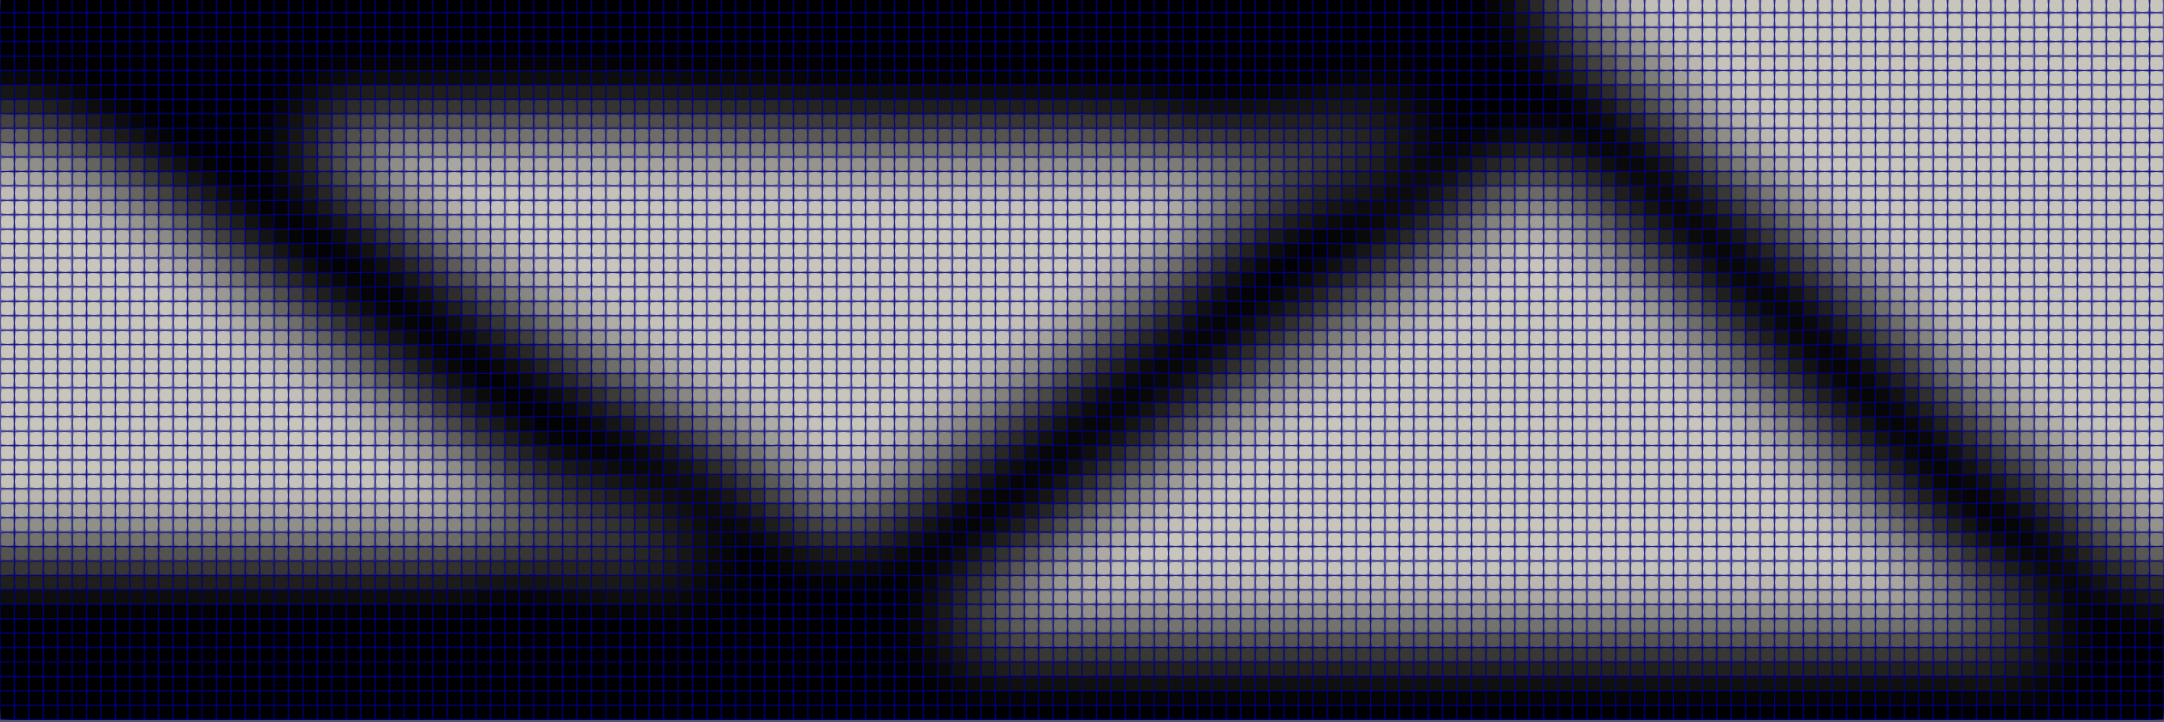
\includegraphics[width=0.5\textwidth]{figures/mbb_dens.png}
		\label{fig:mbb_dens}
	}
	\subfloat[$c(\rho)=191.4873,~v(\rho)=0.5000$]{
		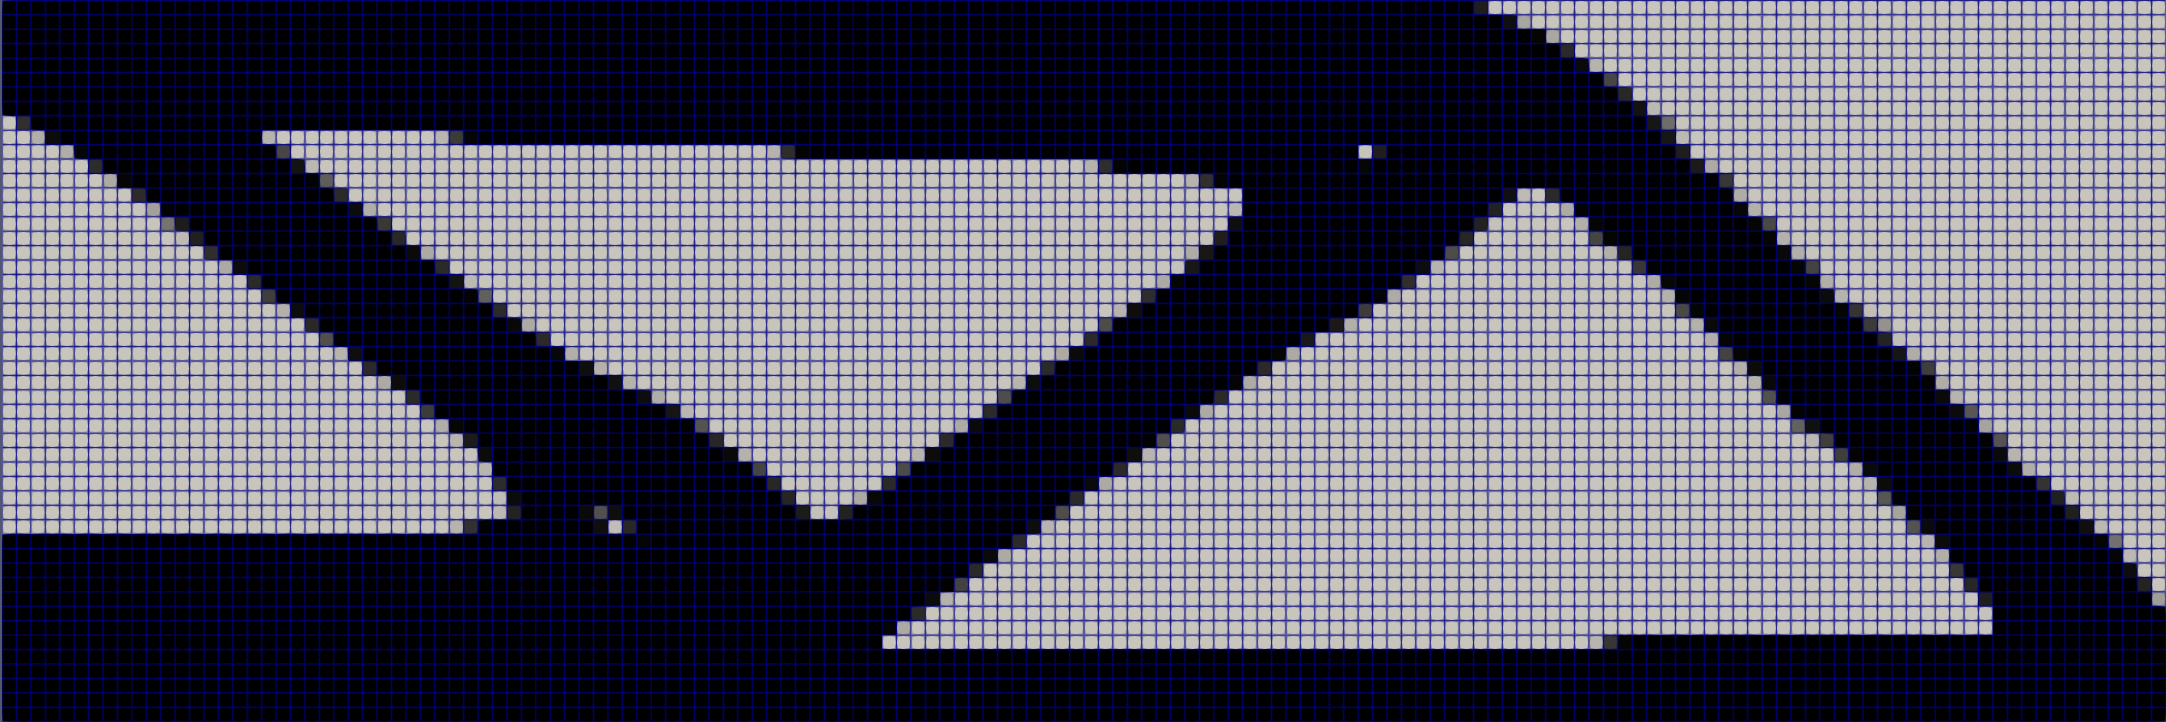
\includegraphics[width=0.5\textwidth]{figures/mbb_heavi.png}
		\label{fig:mbb_heavi}
	}
	\caption{Optimized topologies of the MBB beam using the density filter (left) and the Heaviside projection filter (right).}
	\label{fig:mbb_filter_all}
\end{figure}

As illustrated in the figure, the two filtering strategies result in distinctly different topologies and performance metrics. The density filter produces smoother layouts with blurred structural features, making it more suitable for design scenarios that prioritize continuity and gradual material transitions. In contrast, the Heaviside projection filter yields sharply defined boundaries and well-separated regions, leading to a clearly binarized layout with high visual and structural clarity.

Although the Heaviside filter enforces a minimum feature size through the specified filter radius, small holes with sizes below the threshold may still emerge during the optimization process. This is because the filter emphasizes global binarization rather than strict local geometric control, allowing some fine-scale structures to persist.

In summary, the modular design of SOPTX enables users to switch between different filtering strategies simply by modifying a single line of code. This facilitates efficient exploration of various design intents and helps strike a practical balance between structural smoothness, manufacturability, and binary clarity in TO.

\subsection{Different Optimization Algorithms}
In TO, the choice of optimization algorithm directly affects both computational efficiency and the quality of the resulting design. SOPTX adopts a modular design that enables seamless switching between different optimizers, allowing users to easily tailor optimization strategies to specific design requirements. In this section, we take the MBB beam problem as an example to demonstrate the process of switching from the Optimality Criteria (OC) optimizer to the Method of Moving Asymptotes (MMA). We also present the refactored MMA implementation within SOPTX and highlight its distinctive advantages.

To address complex constrained optimization problems, SOPTX allows users to easily replace the OC optimizer with the more general MMA optimizer by making a simple modification. The switching process only requires importing the \texttt{MMAOptimizer} class and configuring the associated parameters as follows:
\begin{lstlisting}
	from soptx.opt import MMAOptimizer
	
	optimizer = MMAOptimizer(objective=objective,
						constraint=constraint,
						filter_=sens_filter,
						options={'max_iterations': 200, 
								 'tolerance': 0.01})
\end{lstlisting}

In the MBB beam problem, using the same parameters and sensitivity filter as with the OC optimizer, the MMA optimizer produces nearly identical optimized topologies across different meshes. As shown in Figure~\ref{fig:mbb_mma_all}, the relative differences in compliance and volume fraction are both less than $1\%$.  This indicates that although MMA is a more general optimization method, its performance on this specific problem is highly consistent with that of the OC optimizer, demonstrating its reliability and applicability.
\begin{figure}[htp]
	\centering
	\subfloat[$c(\rho)=219.4545,~v(\rho)=0.5000$]{
		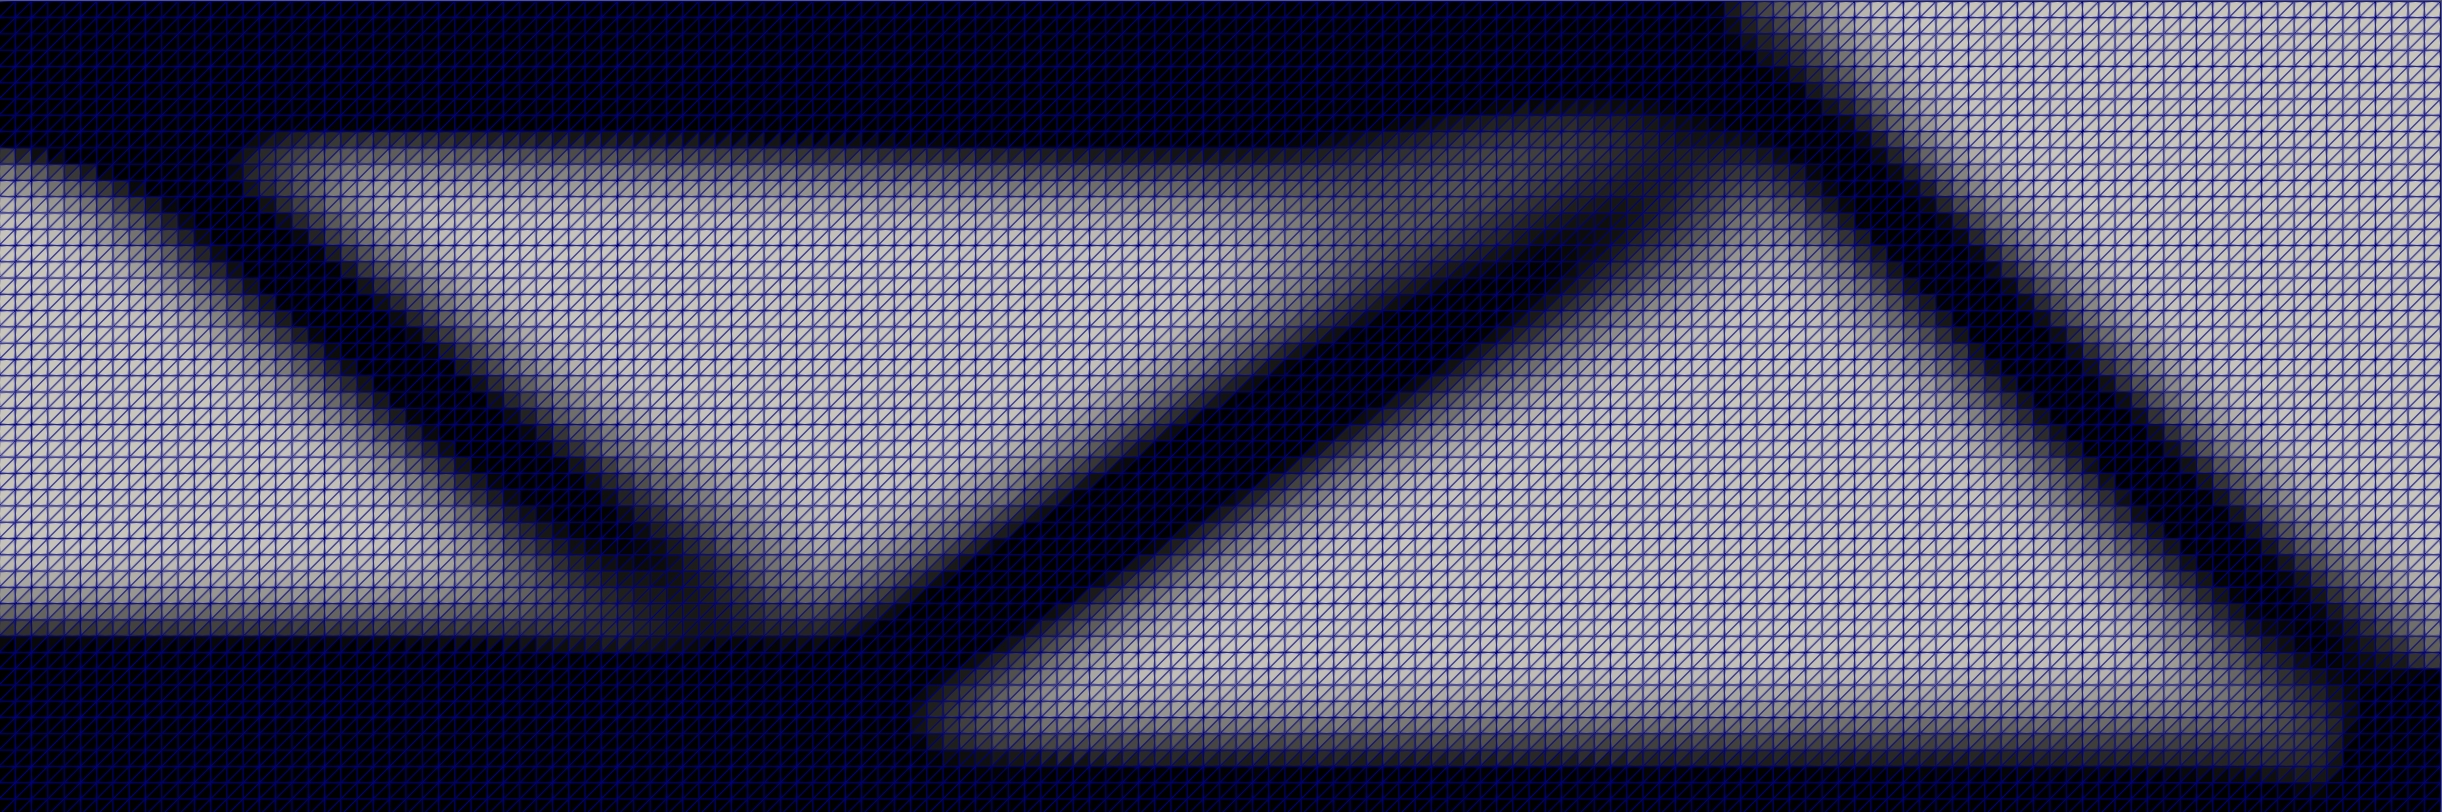
\includegraphics[width=0.5\textwidth]{figures/mbb_mma_u2.png}
		\label{fig:mbb_mma_u2}
	}
	\subfloat[$c(\rho)=220.4377,~v(\rho)=0.4995$]{
		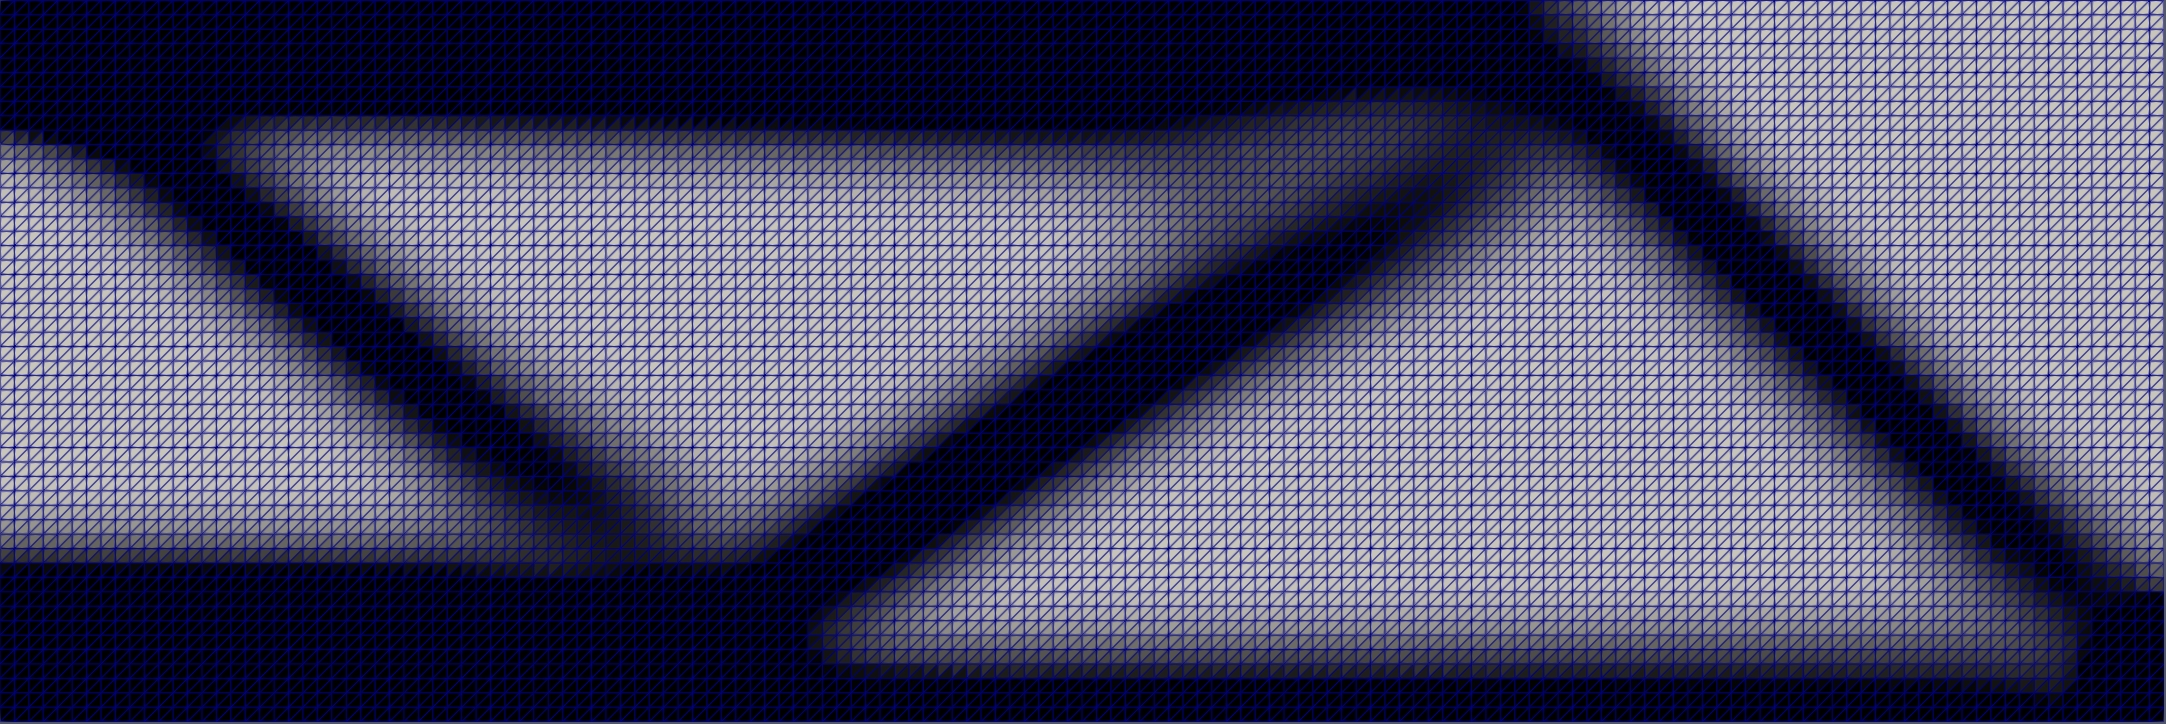
\includegraphics[width=0.5\textwidth]{figures/mbb_mma_tri.png}
		\label{fig:mbb_mma_tri}
	}
	\caption{Optimized topologies of the MBB beam using MMA optimizer on a structured quadrilateral mesh (left) and a triangular mesh (right).}
	\label{fig:mbb_mma_all}
\end{figure}

The MMA algorithm in SOPTX is based on the classical MATLAB implementation provided by Krister Svanberg ~\cite{Svanberg2007MmaAG}, and has been extensively refactored. Unlike traditional MMA implementations commonly found in the literature—where the optimizer is typically treated as a “black box” with limited access to internal mechanisms—the refactored version in SOPTX allows users to conveniently adjust internal algorithmic parameters. These include the number of constraints \texttt{m}, the number of design variables \texttt{n}, the lower and upper bounds \texttt{xmin} and \texttt{xmax}, as well as internal control parameters such as \texttt{a0}, \texttt{a}, \texttt{c}, and \texttt{d}:
\begin{lstlisting}
	optimizer.options.set_advanced_options(
					m=1, n=NC,
					xmin=bm.zeros((NC, 1)),
					xmax=bm.ones((NC, 1)),
					a0=1,
					a=bm.zeros((1, 1)),
					c=1e4 * bm.ones((1, 1)),
					d=bm.zeros((1, 1)),
					)
\end{lstlisting}

Through this refactoring, SOPTX not only enhances the performance of the MMA algorithm but also overcomes the limitations of conventional implementations. It provides users with greater control and cross-platform flexibility, making it particularly advantageous for both research and engineering applications in TO.

\subsection{3D Extension}\label{sec:exp_canti3d}
Thanks to its modular design, SOPTX facilitates a straightforward transition from 2D to 3D models. In this section, we demonstrate the capability of SOPTX in solving 3D TO problems through the compliance minimization of a 3D cantilever beam, as illustrated in Figure~\ref{fig:cantilever_3d}. The beam is fully fixed on the left end, and a downward concentrated load of magnitude $T=-1$ is applied at the bottom of the right end. A structured uniform grid of hexahedral elements with size $60\times20\times4$ is employed. The target volume fraction is set to $0.3$, and the material parameters are $E = 1$ and $\nu = 0.3$. The SIMP penalty factor is chosen as $p=3$. A sensitivity filter with radius $r=1.5$ (matched to the mesh element size) is used to ensure structural smoothness and suppress checkerboard patterns.
\begin{figure}[htp]
	\centering
	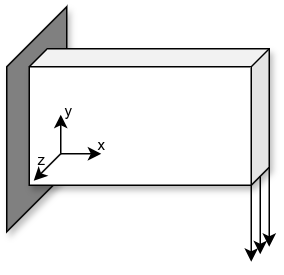
\includegraphics[width=0.6\textwidth]{figures/cantilever_3d.png}
	\caption{Geometric configuration of the 3D cantilever beam. The left end is fully fixed, and a downward concentrated load is applied at the bottom of the right end.}
	\label{fig:cantilever_3d}
\end{figure}

Compared to the 2D cantilever beam example in Section~\ref{sec:exp_canti_beam}, SOPTX can be seamlessly extended to the 3D cantilever beam problem by simply replacing the PDE model and mesh configuration. The 3D cantilever beam model is implemented via the \texttt{Cantilever3dData1} class, as shown below, and the complete code definition is available in \ref{sec:code_canti_3d}
\begin{lstlisting}
	from soptx.pde import Cantilever3dData1
	pde = Cantilever3dData1(xmin=0, xmax=60, ymin=0, ymax=20, zmin=0, zmax=4, T = -1)
	
	from fealpy.mesh import UniformMesh3d
	mesh = UniformMesh3d(extent=[0, 60, 0, 20, 0, 4], h=[1, 1, 1], origin=[0, 0, 0])
\end{lstlisting}

The initial material density is uniformly set to the target volume fraction of $0.3$. Using the OC optimizer and a sensitivity filter with radius $r=1.5$, the convergence histories of the compliance $c(\rho)$ and the volume fraction $v(\rho)$ are shown in Figure~\ref{fig:canti_3d_convergence}. The compliance drops rapidly from an initial value of approximately $28000$ to around $5000$ within the first 6 iterations. It then decreases more gradually, fluctuating slightly between iterations 6 and 20 before settling to about $2000$. Smooth convergence is eventually achieved at iteration 54. The volume fraction remains nearly constant around $0.3$ throughout the process, indicating effective constraint control.
\begin{figure}[htp]
	\centering
	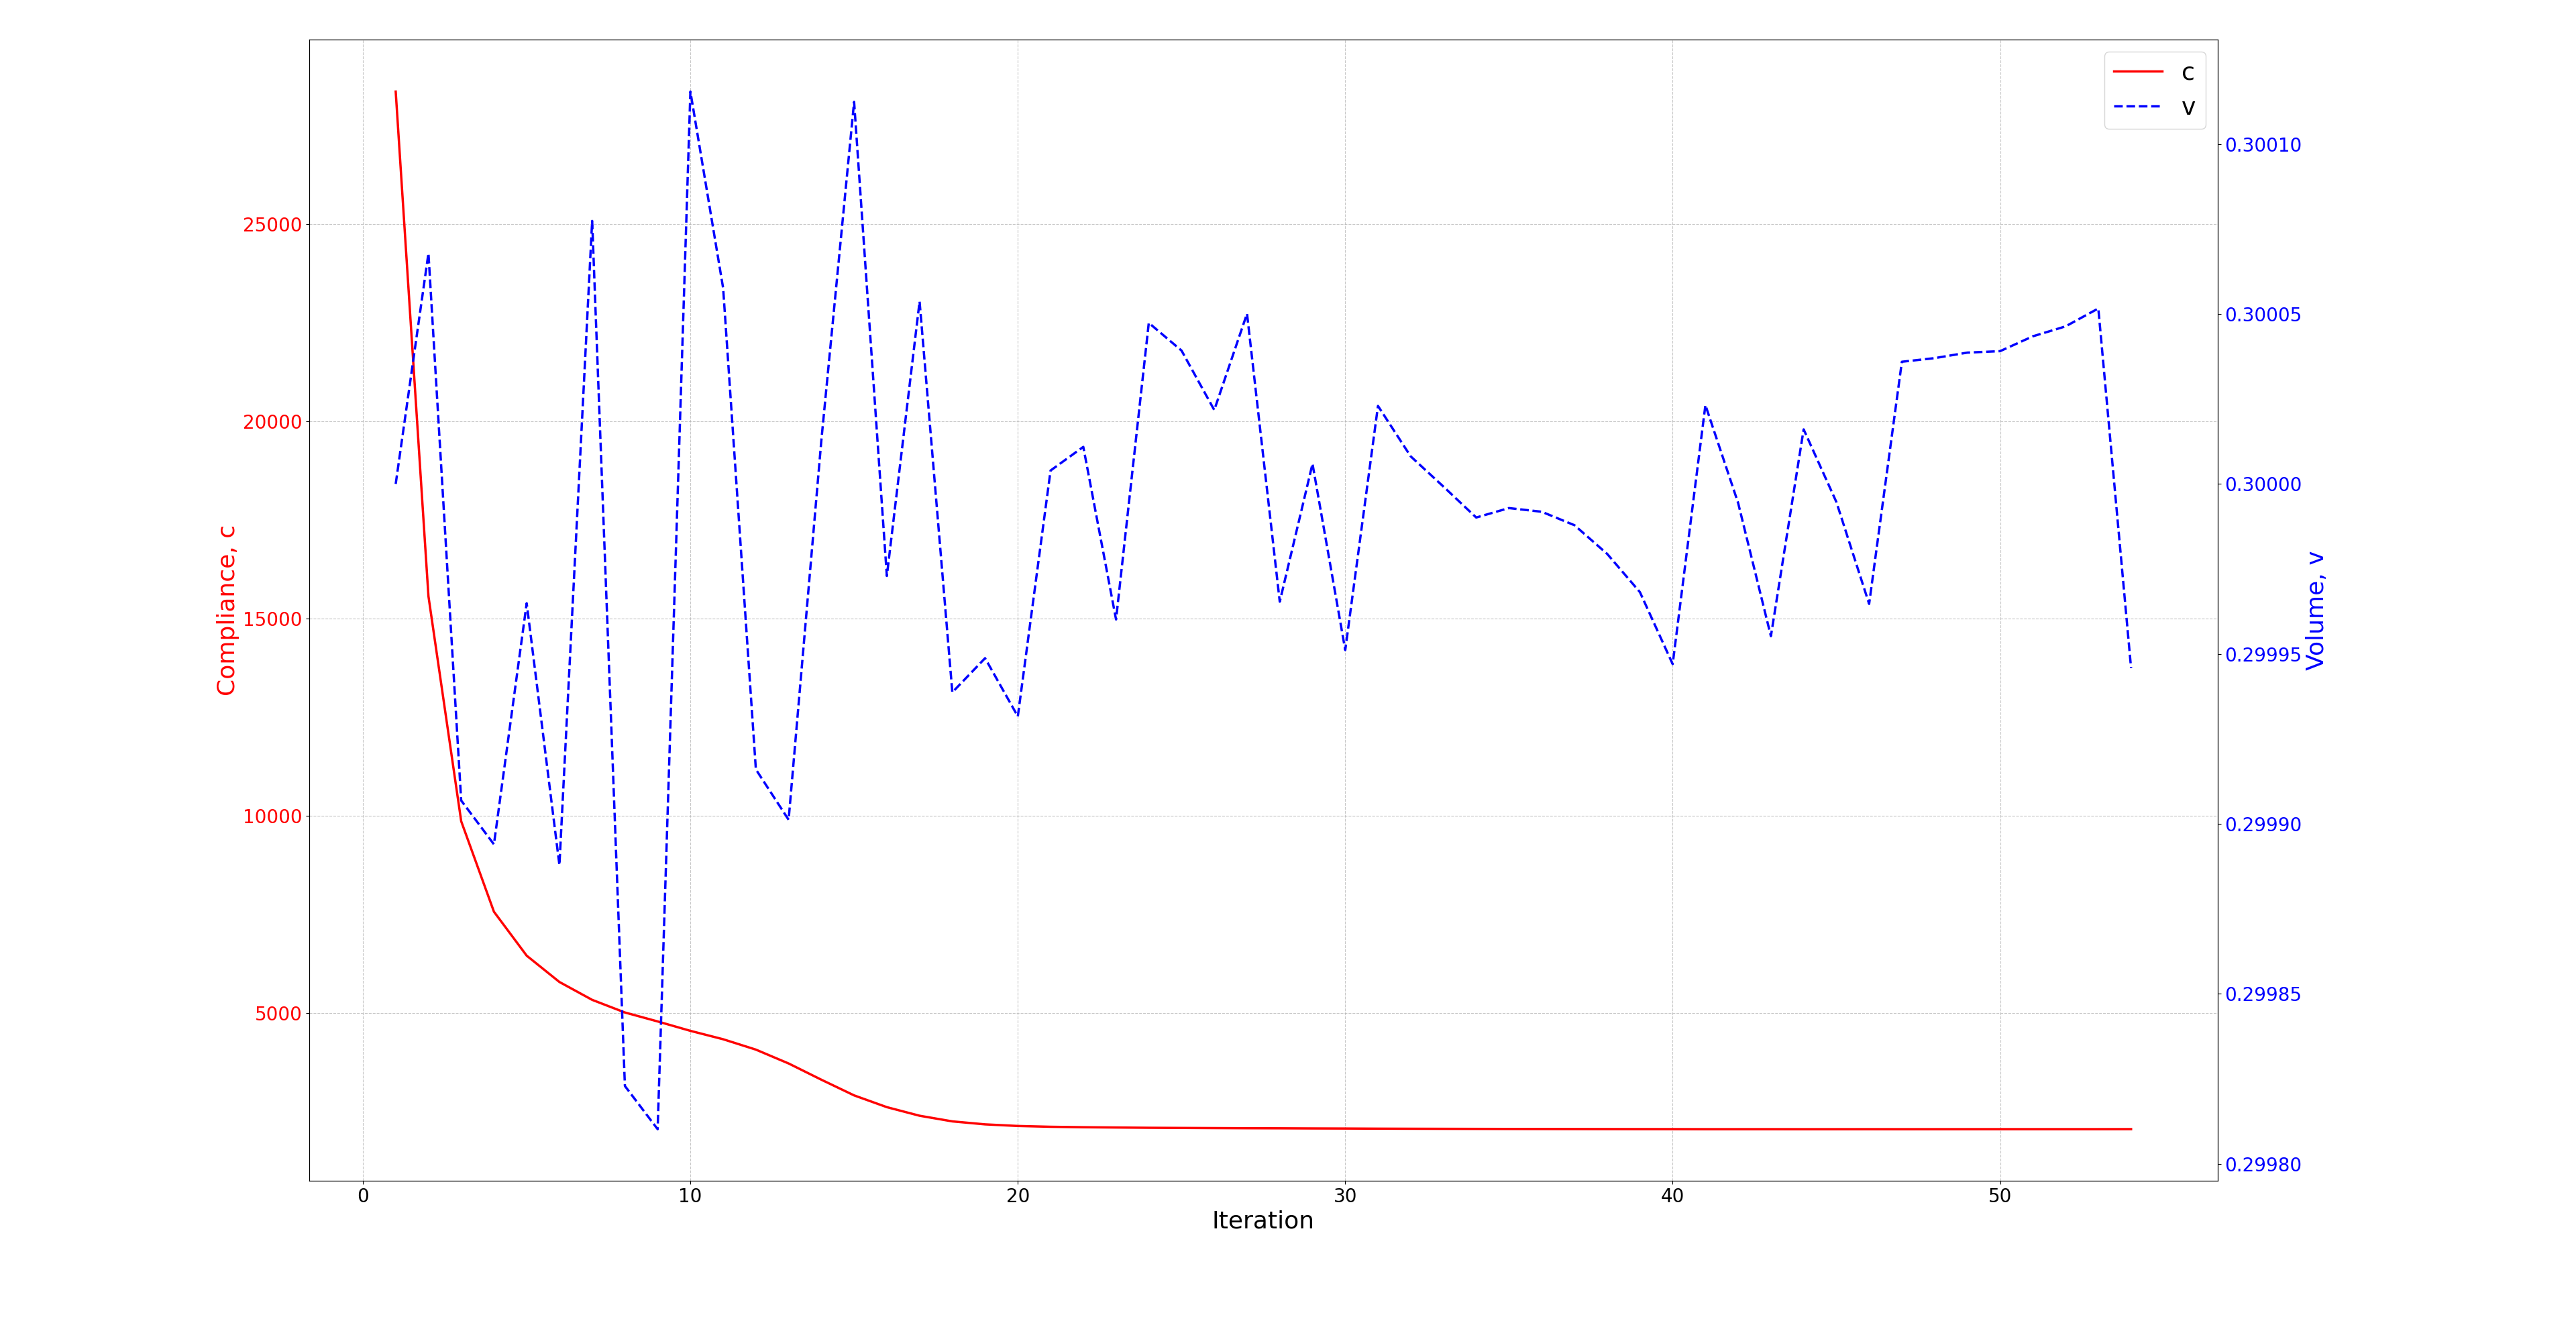
\includegraphics[width=1.0\textwidth]{figures/cantilever_3d_convergence.png}
	\caption{Convergence histories of the compliance $c(\rho)$ and volume fraction $v(\rho)$ for the 3D cantilever beam initialized with a uniform density of $0.3$.}
	\label{fig:canti_3d_convergence}
\end{figure}

To better visualize the optimization results, Figure~\ref{fig:canti3d_all} shows the topology layouts at iterations 7, 21, and 54. Only elements with density values $\rho > 0.3$ are rendered to highlight the structural features.
\begin{figure}[htp]
	\centering
	\subfloat[$c(\rho)=5338.9462,~v(\rho)=0.3001$]{
		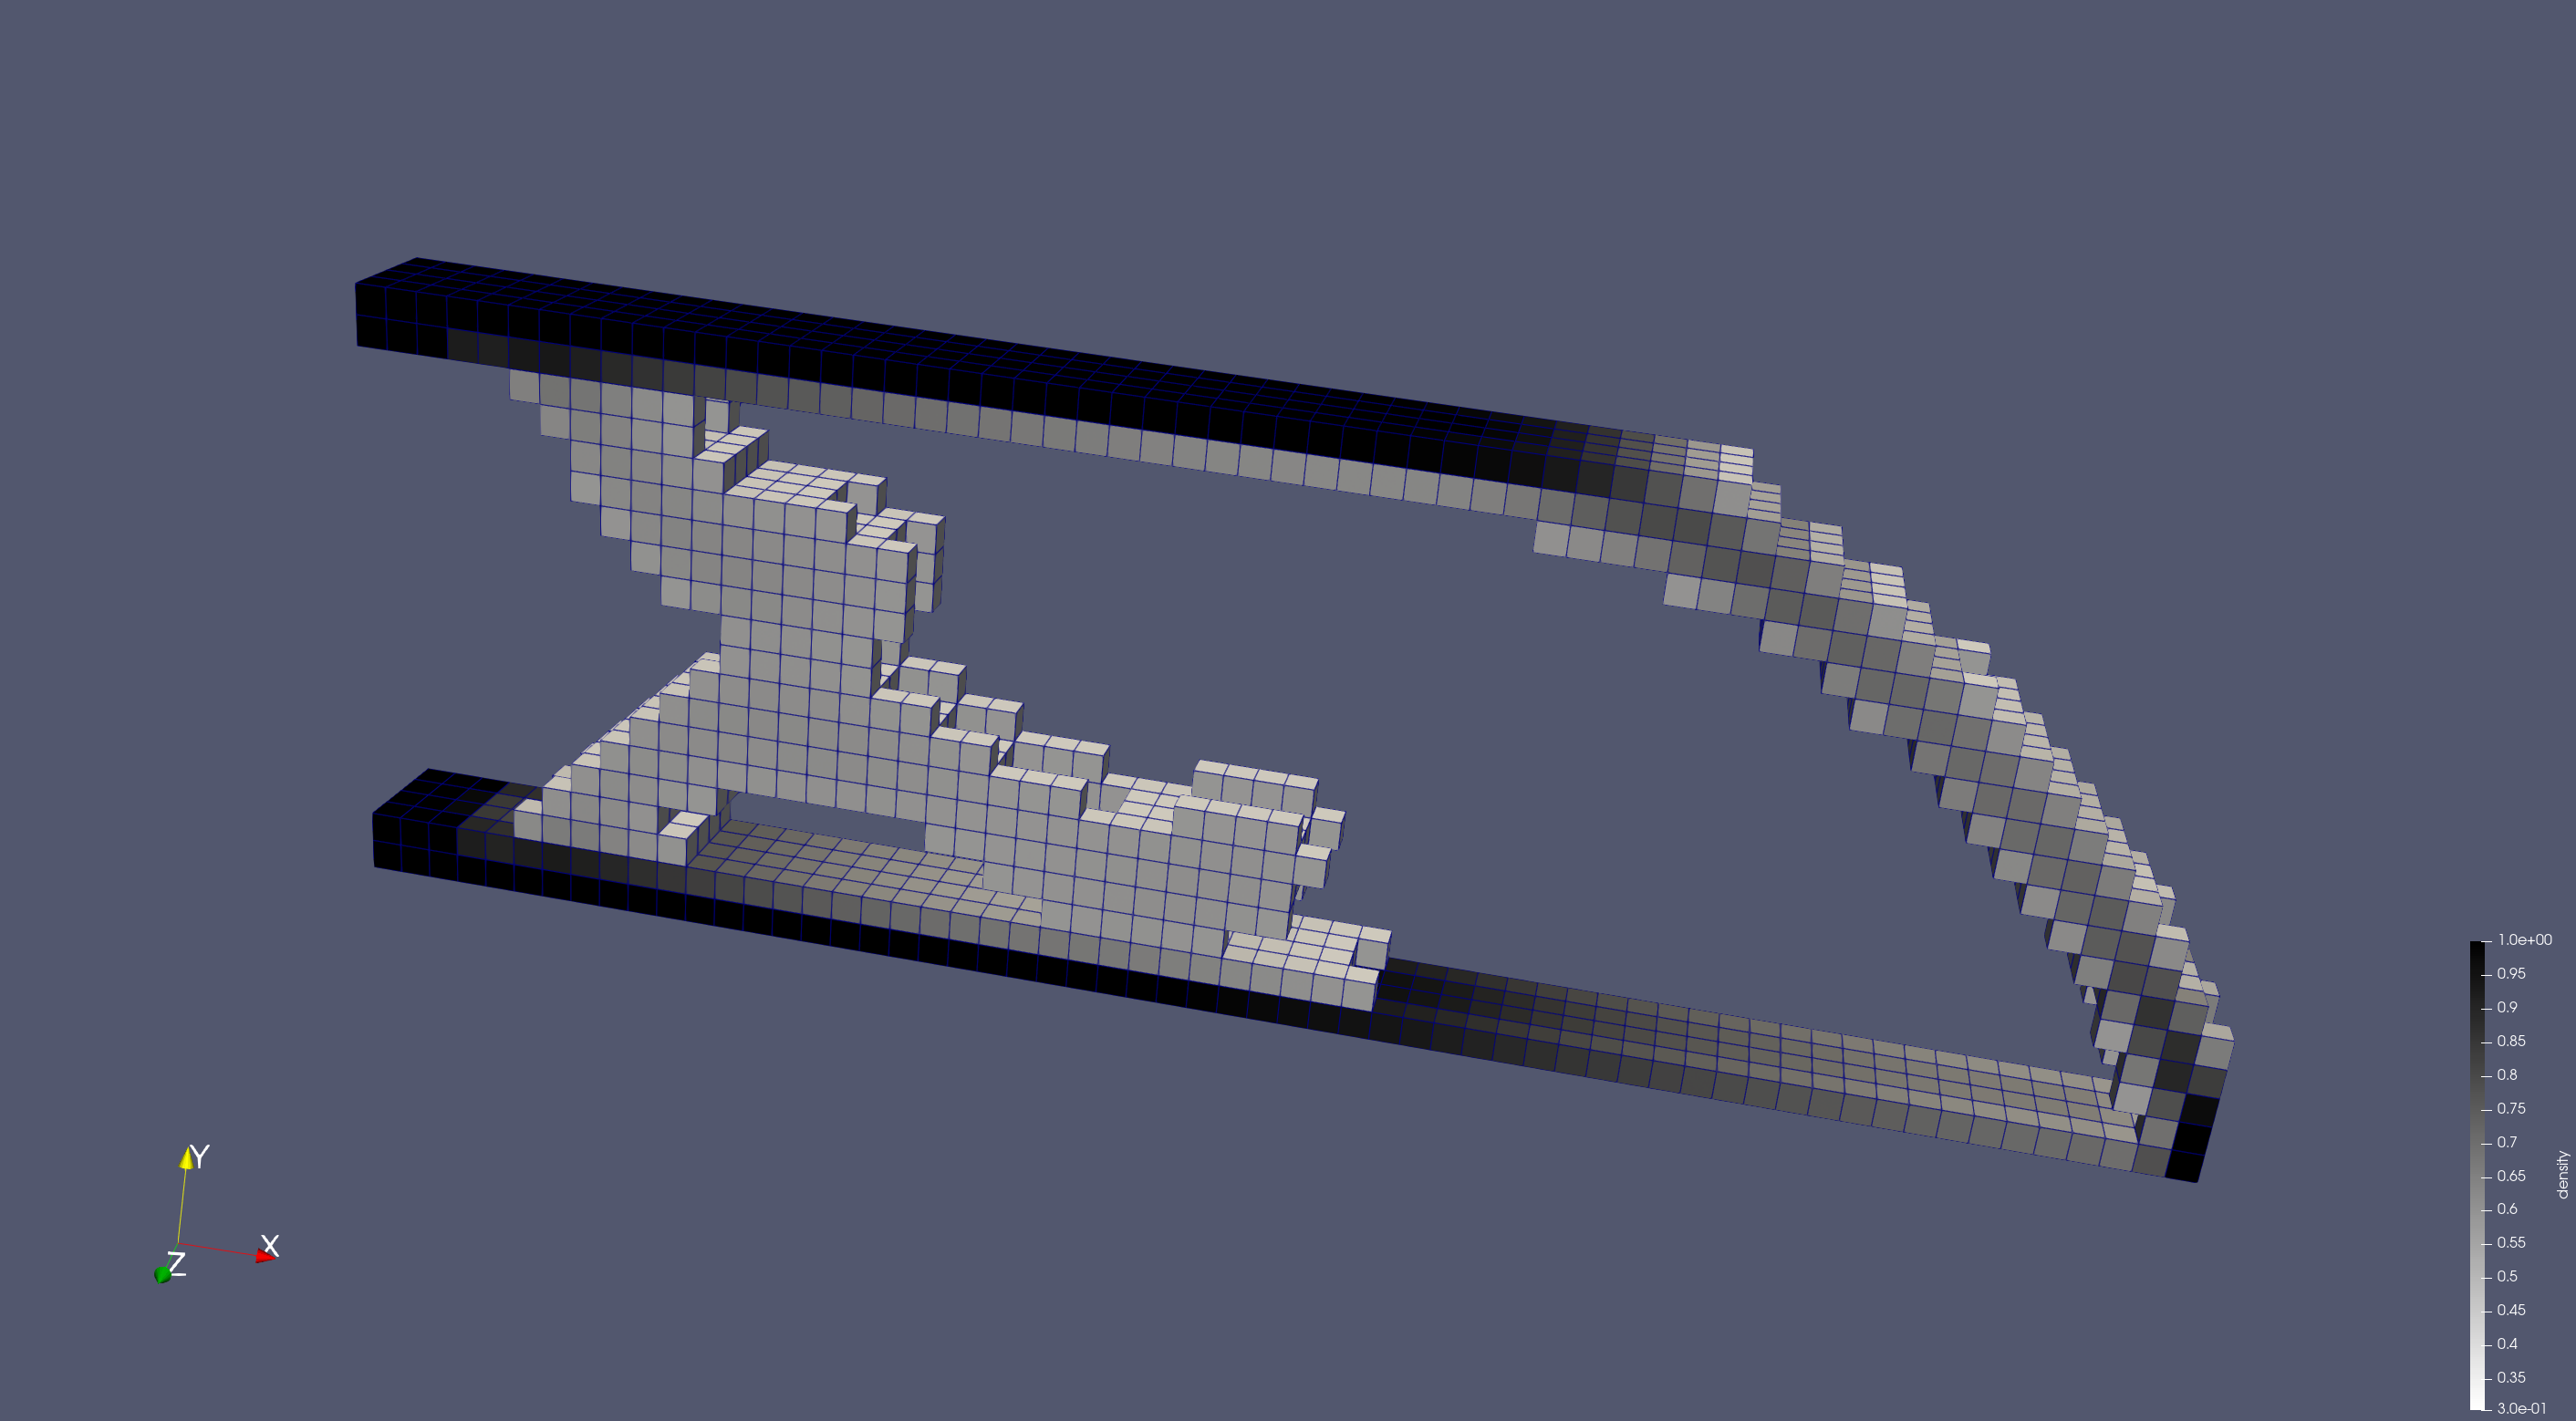
\includegraphics[width=0.32\textwidth]{figures/cantilever_3d_1.png}
		\label{fig:canti3d_1}
	}
	\subfloat[$c(\rho)=2122.6707,~v(\rho)=0.3000$]{
		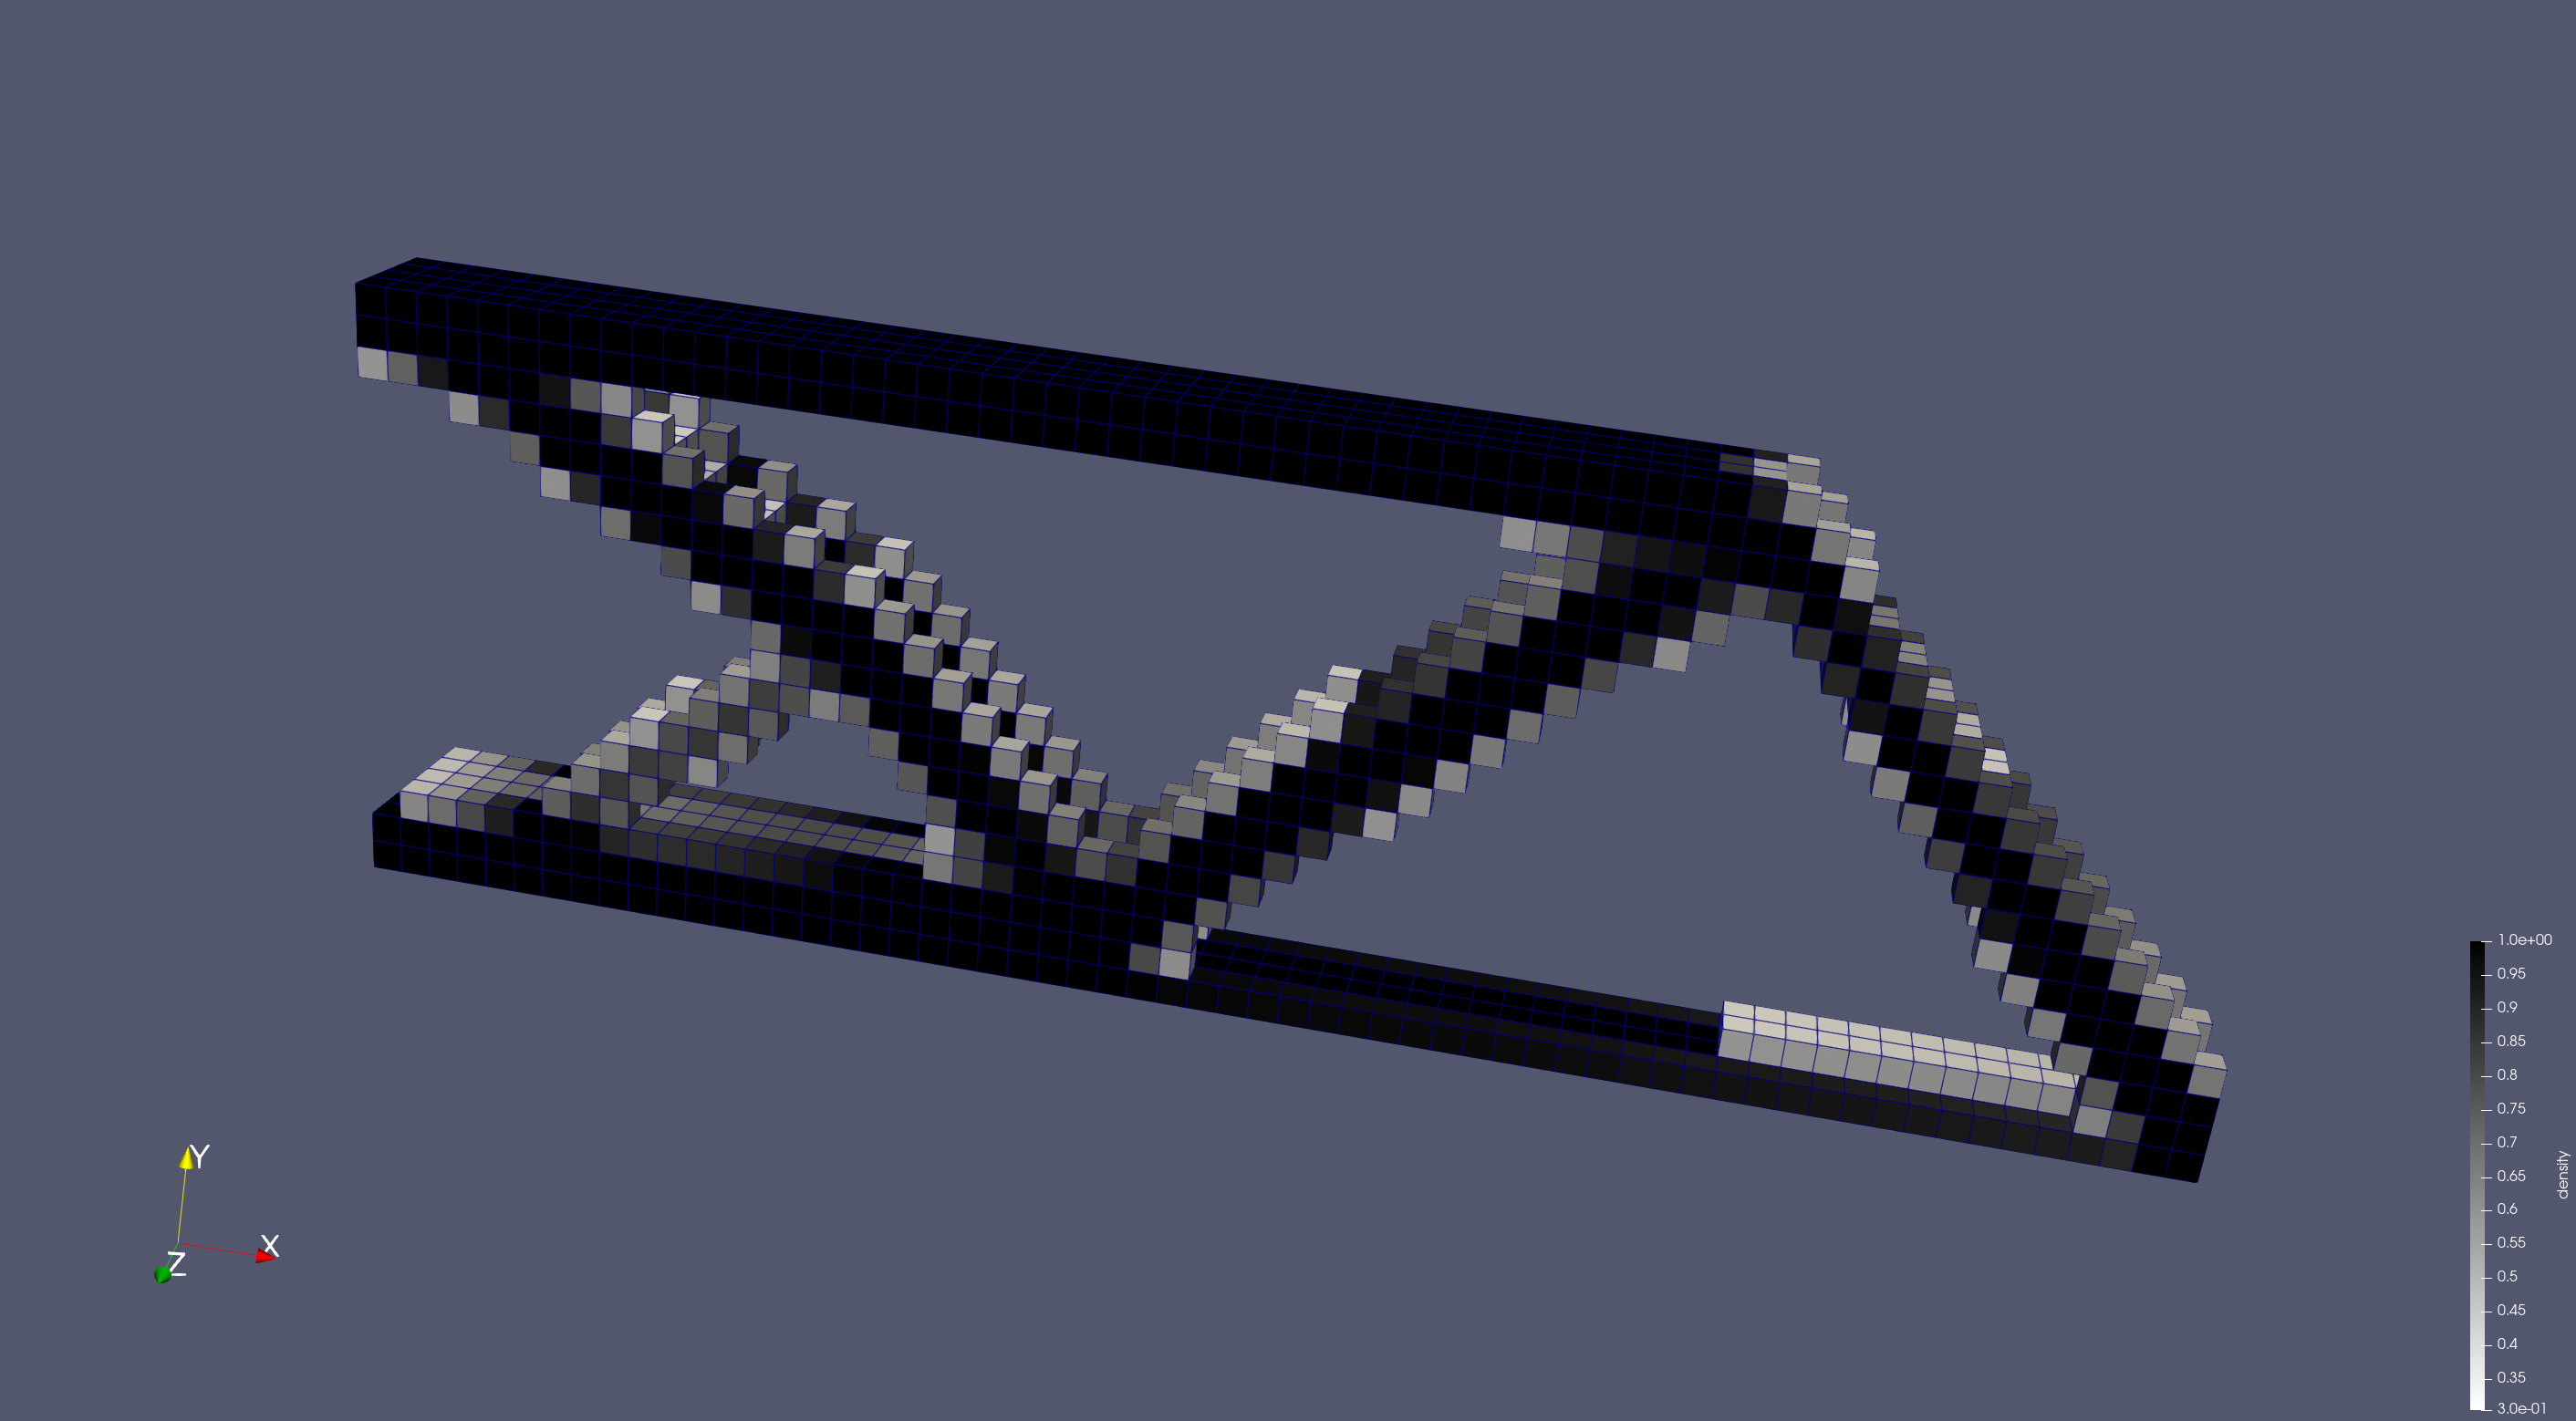
\includegraphics[width=0.32\textwidth]{figures/cantilever_3d_2.png}
		\label{fig:canti3d_2}
	}
	\subfloat[$c(\rho)=2063.5625,~v(\rho)=0.2999$]{
		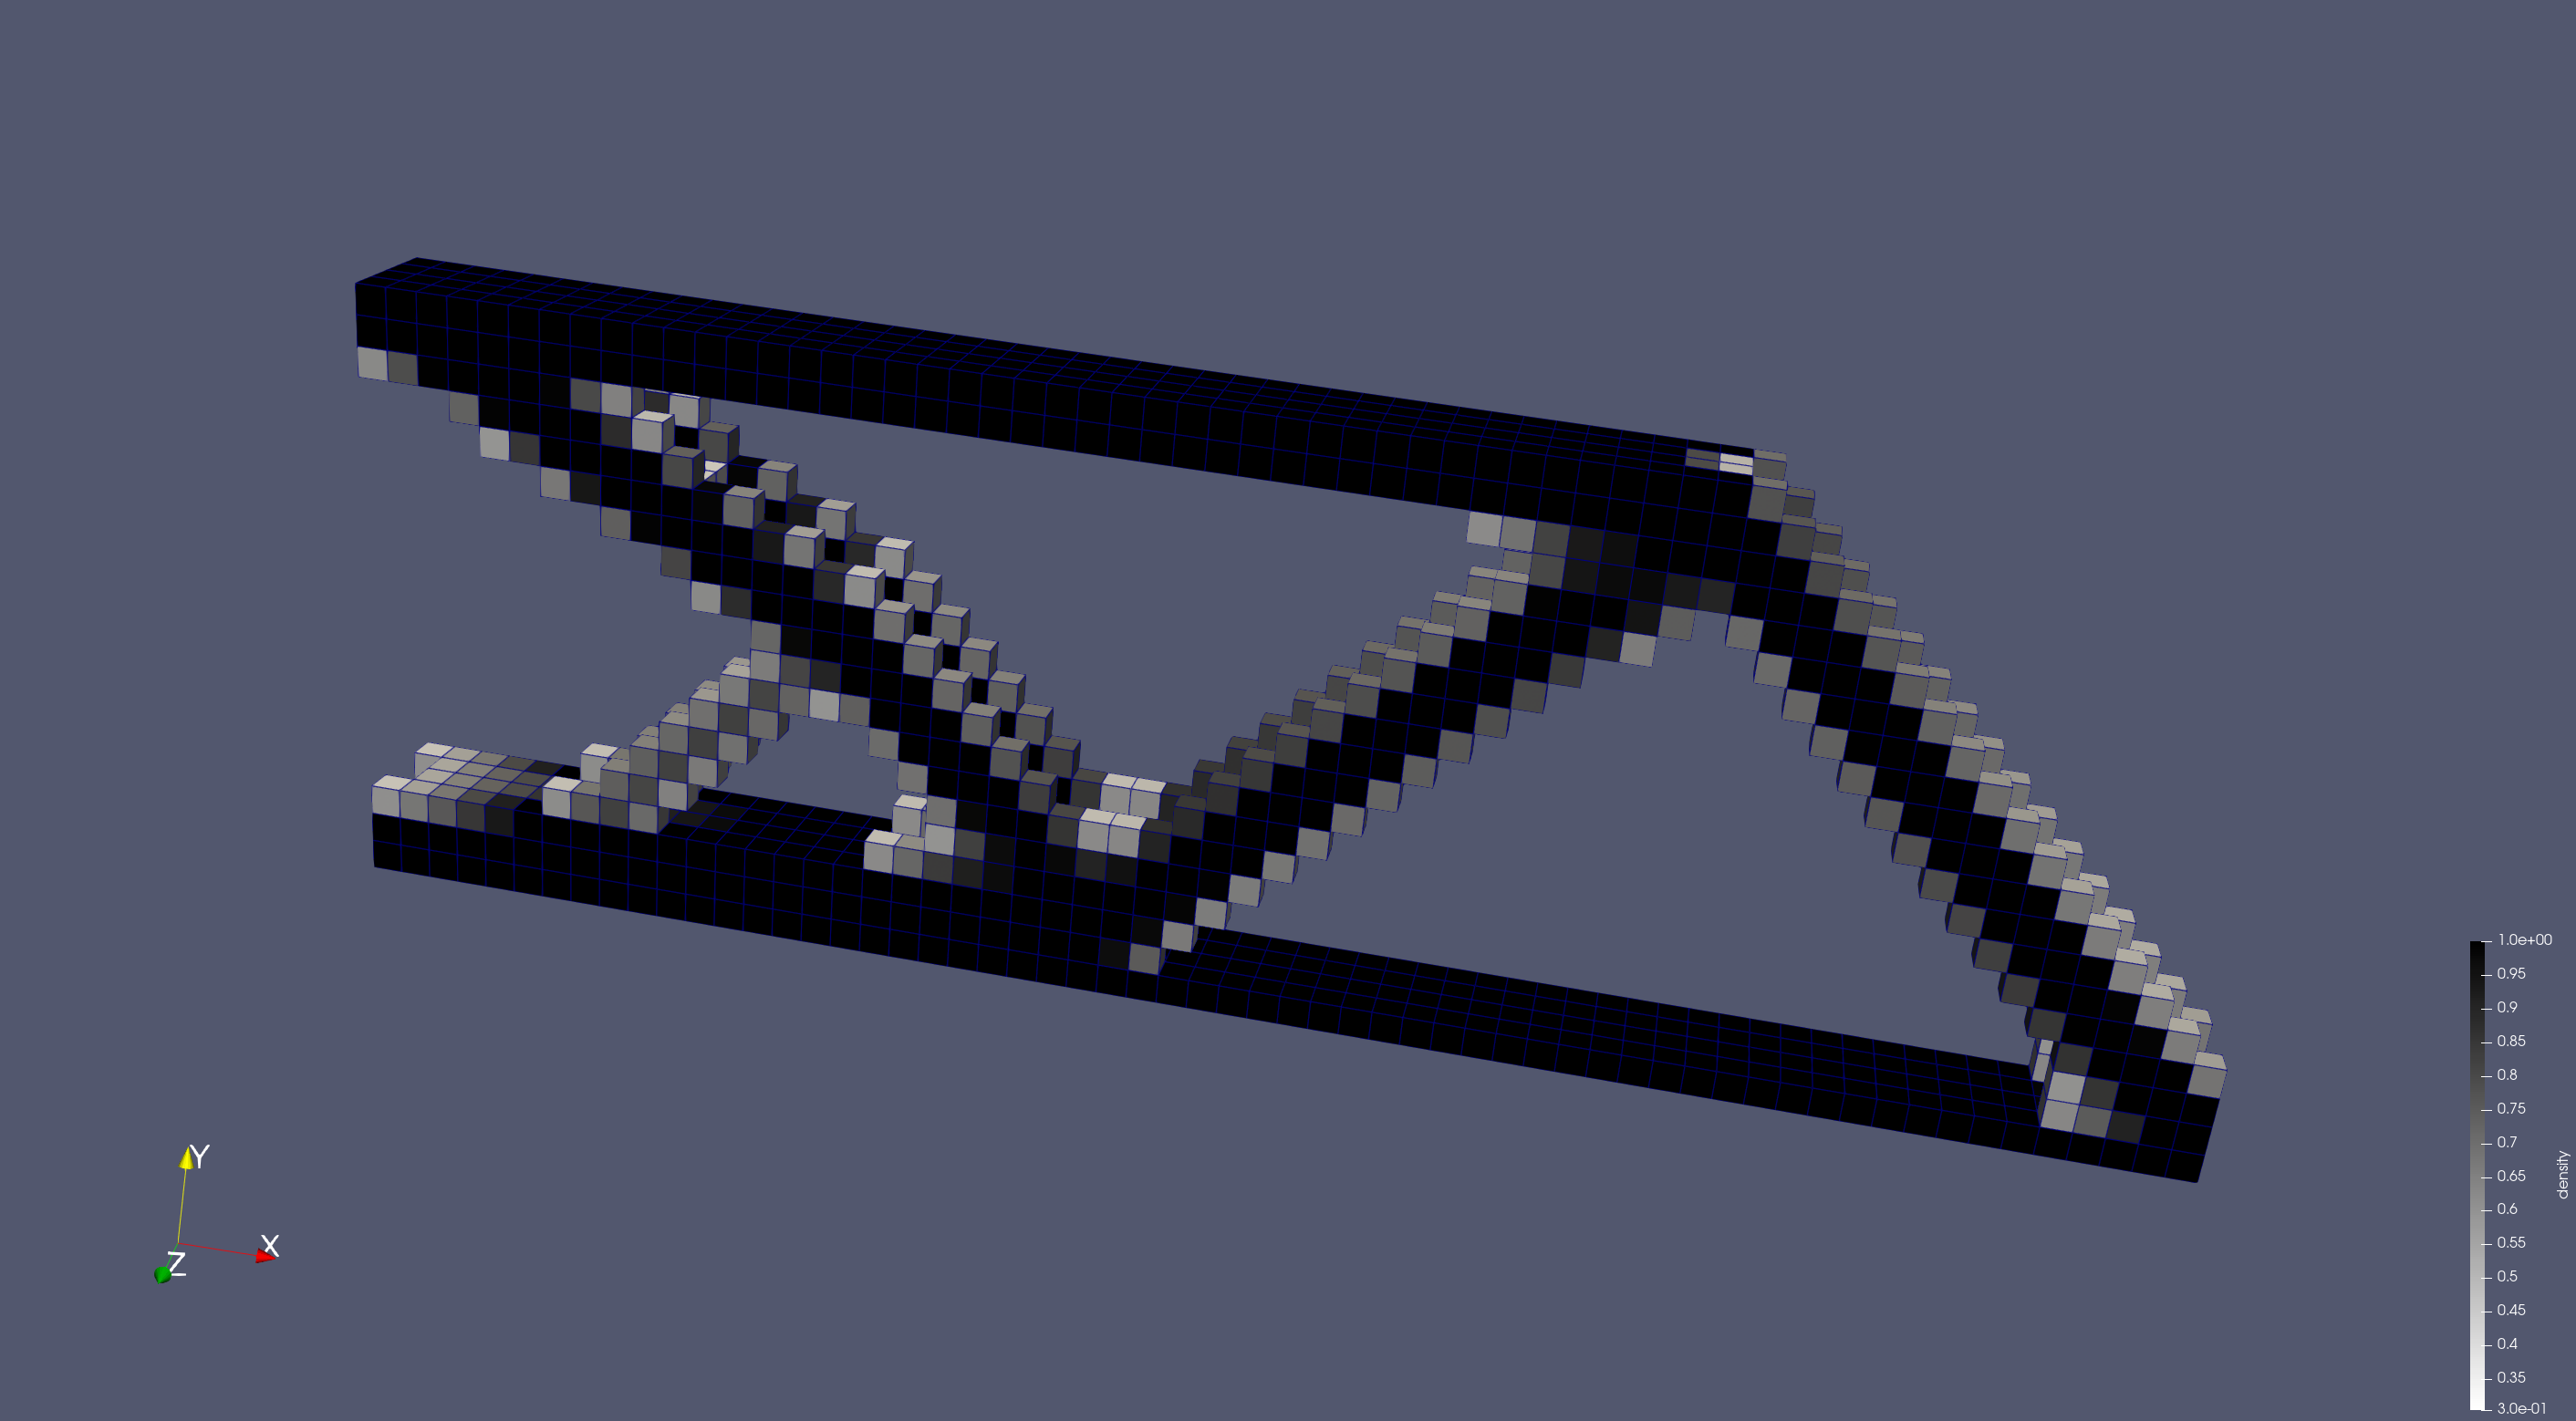
\includegraphics[width=0.32\textwidth]{figures/cantilever_3d_3.png}
		\label{fig:canti3d_3}
	}
	\caption{Topology layouts at iterations 7, 21, and 54 during the optimization of the 3D cantilever beam. Elements with $\rho > 0.3$ are visualized. Each subfigure also reports the compliance and volume fraction.}
	\label{fig:canti3d_all}
\end{figure}

It is worth noting that, compared to 2D problems, 3D TO significantly increases computational complexity. This is particularly evident when using large-scale meshes, where both computational cost and memory requirements grow substantially. The SOPTX framework addresses these challenges through efficient matrix assembly and support for multiple computational backends, demonstrating excellent extensibility and computational performance. The implementation details of these features will be elaborated in the following sections.

\subsection{Application of Fast Matrix Assembly}
In 3D TO problems, computational efficiency is a central challenge. Taking the 3D cantilever beam example from Section~\ref{sec:exp_canti3d} as a representative case, the mesh consists of $60\times20\times4$ elements, resulting in $19,215$ displacement degrees of freedom and $4,800$ density variables. The optimization process requires 54 iterations in total. In traditional finite element methods, the assembly of the global stiffness matrix often involves a large number of redundant numerical integration operations, which becomes the primary bottleneck in the overall computational workflow.

To overcome this bottleneck, the SOPTX framework incorporates a fast matrix assembly technique, which separates the element-dependent and element-independent parts of stiffness matrix computation. This decomposition enables efficient evaluation and reuse of invariant quantities, significantly accelerating the assembly process. In addition, to further improve the accuracy of matrix assembly, SOPTX implements a symbolic integration precomputation technique. This approach analytically integrates the element-independent components using symbolic computation in advance, eliminating numerical integration errors and enhancing both numerical stability and overall accuracy.
\begin{itemize} 
	\item \textbf{Fast matrix assembly}: Accelerates matrix assembly by separating element-dependent and element-independent terms, coupled with efficient numerical integration.
	\item \textbf{Symbolic integration precomputation}: Further improves accuracy and stability by analytically integrating invariant terms ahead of time.
\end{itemize}

Moreover, SOPTX employs intelligent caching to store invariant data across iterations, enabling direct reuse and substantially reducing average computational time in later iterations.

Table~\ref{tab:assembly_comparison} summarizes the performance of different matrix assembly techniques under the same problem setting of the 3D cantilever beam optimization described in Section~\ref{sec:exp_canti3d}.
\begin{table}[htbp]
	\centering
%	\setlength{\tabcolsep}{4pt} % 减小列间距
	\caption{Performance comparison of matrix assembly techniques in the 3D cantilever beam optimization problem. All values are reported in seconds.}
%	\small % 使用小字体
	\begin{tabular}{cccccc}
		\toprule
		\textbf{Assembly Technique} & \textbf{Total} & \textbf{1st Iter.} & \textbf{1st Assembly} & \textbf{Avg. Iter.} & \textbf{Avg. Assembly} \\
		\midrule
		Original Assembly & 68.605 & 3.342 & 1.197 & 1.231 & 0.838 \\
		Fast Assembly & 39.826 & 2.387 & 0.342 & 0.706 & 0.276 \\
		Symbolic Fast Assembly & 41.194 & 5.877 & 3.853 & 0.666 & 0.272 \\
		\bottomrule
	\end{tabular}
	\label{tab:assembly_comparison}
\end{table}

As shown in Table~\ref{tab:assembly_comparison}, the original matrix assembly method results in an average assembly time of \SI{0.838}{s} per iteration after the first one, accounting for approximately $68\%$ of the total iteration time. This clearly constitutes a performance bottleneck. With the adoption of the fast matrix assembly technique, the average assembly time is reduced to \SI{0.276}{s}---only about $33\%$ of that of the original method. Although the symbolic fast assembly method incurs a longer initialization time of \SI{3.853}{s} during the first iteration, it achieves the lowest average assembly time in subsequent iterations (\SI{0.272}{s}), while ensuring analytical accuracy in integration.

In summary, the matrix fast assembly strategy implemented in SOPTX effectively reduces the computational cost of topology optimization and improves both numerical accuracy and stability. This makes it particularly well suited for solving large-scale topology optimization problems with stringent demands on computational efficiency and precision.

\subsection{Application of Automatic Differentiation}\label{sec:exp_canti3d_ad}
Sensitivity analysis is a core component of TO, guiding the update of design variables. Traditional methods typically require manual derivation and implementation of sensitivity formulas, which can be time-consuming and error-prone, especially for complex material models or constraint conditions. The SOPTX framework introduces AD to automate sensitivity computations, allowing users to focus on problem modeling and solution strategies without dealing with tedious mathematical derivations. In this section, we use the 3D cantilever beam example from Section~\ref{sec:exp_canti3d} to demonstrate how SOPTX leverages AD to compute the sensitivities of the compliance objective and the volume constraint. The advantages and application scenarios of AD in TO are also discussed.

The SOPTX framework supports multiple computational backends, including NumPy, PyTorch, and JAX. While FEALPy by default operates with the NumPy backend~\cite{harris2020array}, NumPy does not support AD. Therefore, users need to switch to a backend that supports AD in order to enable this functionality. For example, switching to the PyTorch backend~\cite{paszke2017automatic} requires only a single line of code:
\begin{lstlisting}[language=bash]
	bm.set_backend('pytorch')
\end{lstlisting}

In SOPTX, the mode of sensitivity computation for objective and constraint functions is controlled by the configuration parameter \texttt{diff\_mode}. By default, \texttt{diff\_mode} is set to \texttt{'manual'}, meaning that manually derived sensitivity expressions are used. To enable AD, users simply set \texttt{diff\_mode} to \texttt{'auto'}. The following code snippet shows how to enable AD for the structural compliance objective while retaining manual differentiation for the volume constraint:
\begin{lstlisting}[language=bash]
	obj_config = ComplianceConfig(diff_mode='auto')
	objective = ComplianceObjective(solver=solver, config=obj_config)
	
	cons_config = VolumeConfig(diff_mode='manual')
	constraint = VolumeConstraint(solver=solver, volume_fraction=0.5, config=cons_config)
\end{lstlisting}

Under this configuration, the sensitivity of the compliance objective is computed automatically via AD, whereas the sensitivity of the volume constraint remains manually derived. This flexibility allows users to selectively choose the most appropriate differentiation method according to the problem requirements. The detailed implementation of the compliance sensitivity computation using AD is provided in~\ref{sec:ad_compliance}

To verify the correctness and effectiveness of AD, we conduct tests using the 3D cantilever beam problem described in Section~\ref{sec:exp_canti3d}. All parameters are kept identical: the mesh size is $60\times20\times4$, the target volume fraction is set to $0.3$,  the initial material density is $0.3$, material properties are $E=1$ and $\nu=0.3$, the SIMP penalty factor is $p=3$, and the sensitivity filter radius is $r=1.5$. The structural compliance sensitivity is computed using AD. Figure~\ref{fig:canti3d_ad_convergence} shows the convergence histories of the compliance and volume fraction.

\begin{figure}[htp] 
	\centering 
	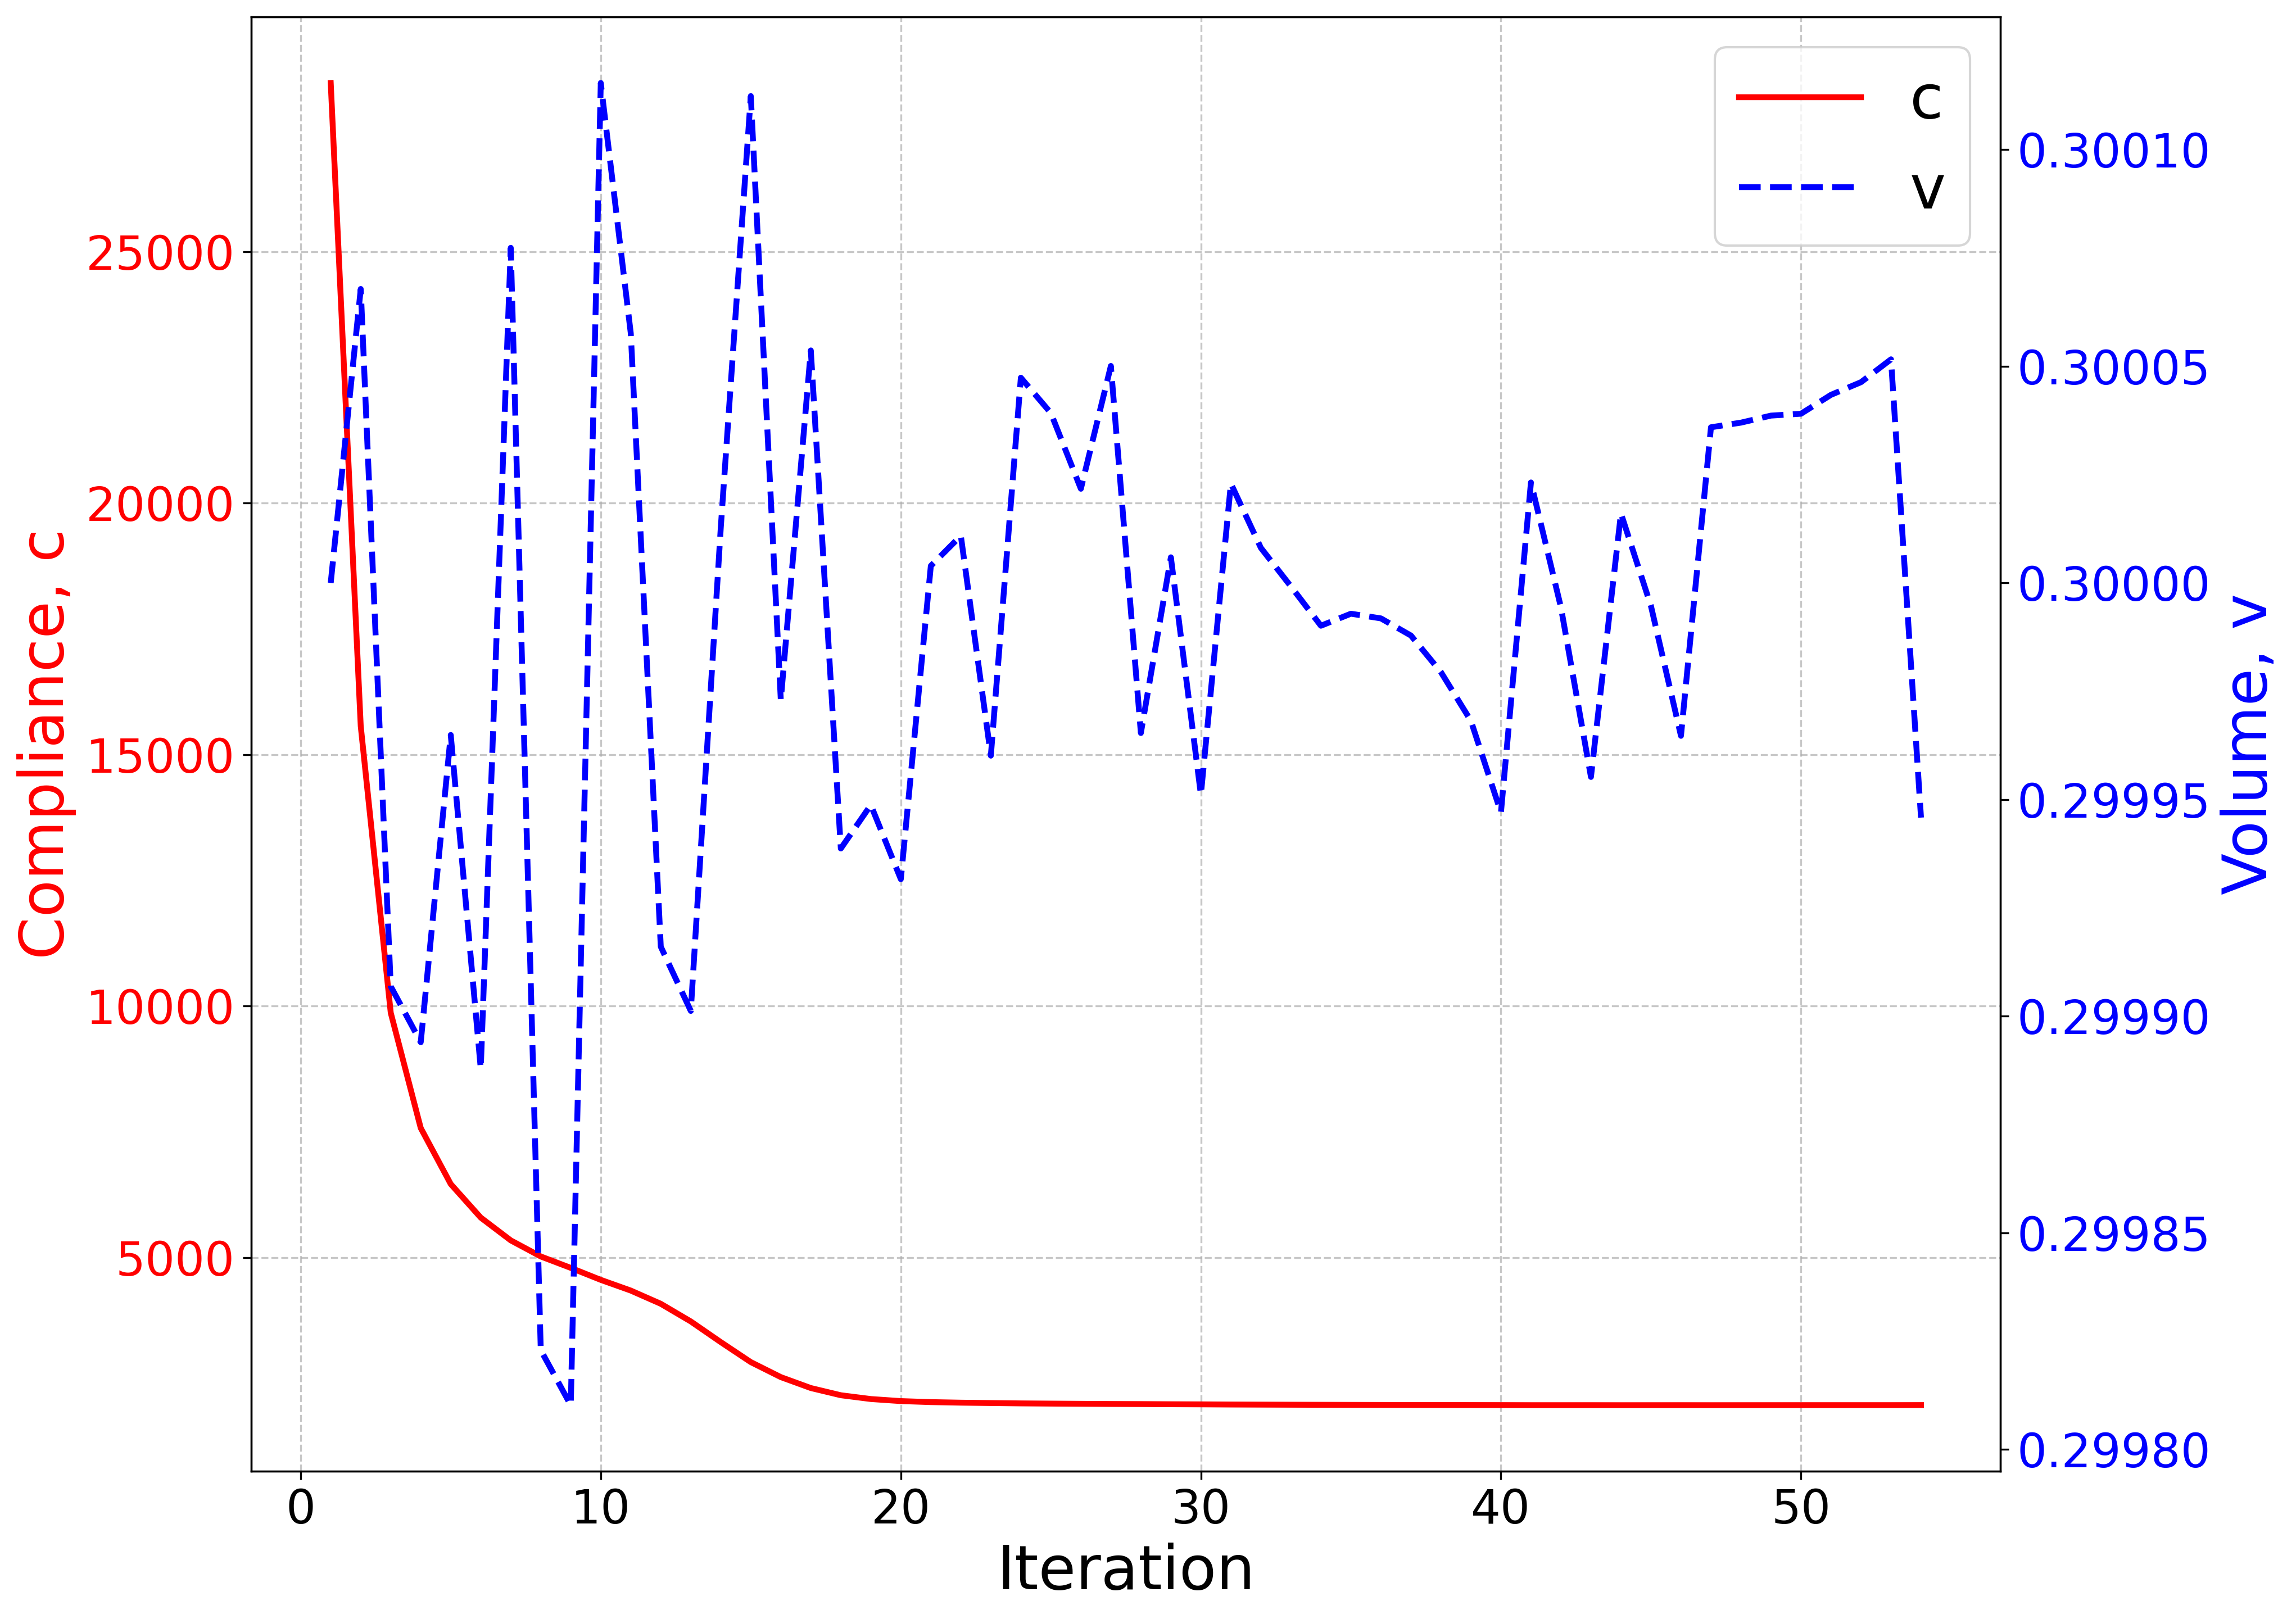
\includegraphics[width=1.0\textwidth]{figures/cantilever_3d_convergence_auto.png} \caption{Convergence histories of the compliance $c(\rho)$ and volume fraction $v(\rho)$ for the 3D cantilever beam optimization using automatic differentiation.} \label{fig:canti3d_ad_convergence} 
\end{figure}

To further illustrate the evolution of the topology during optimization, the layouts at selected iterations are shown in Figure~\ref{fig:canti3d_ad_topos}.

\begin{figure}[htp]
	\centering
	\subfloat[$c(\rho)=5338.9462,~v(\rho)=0.3001$]{
		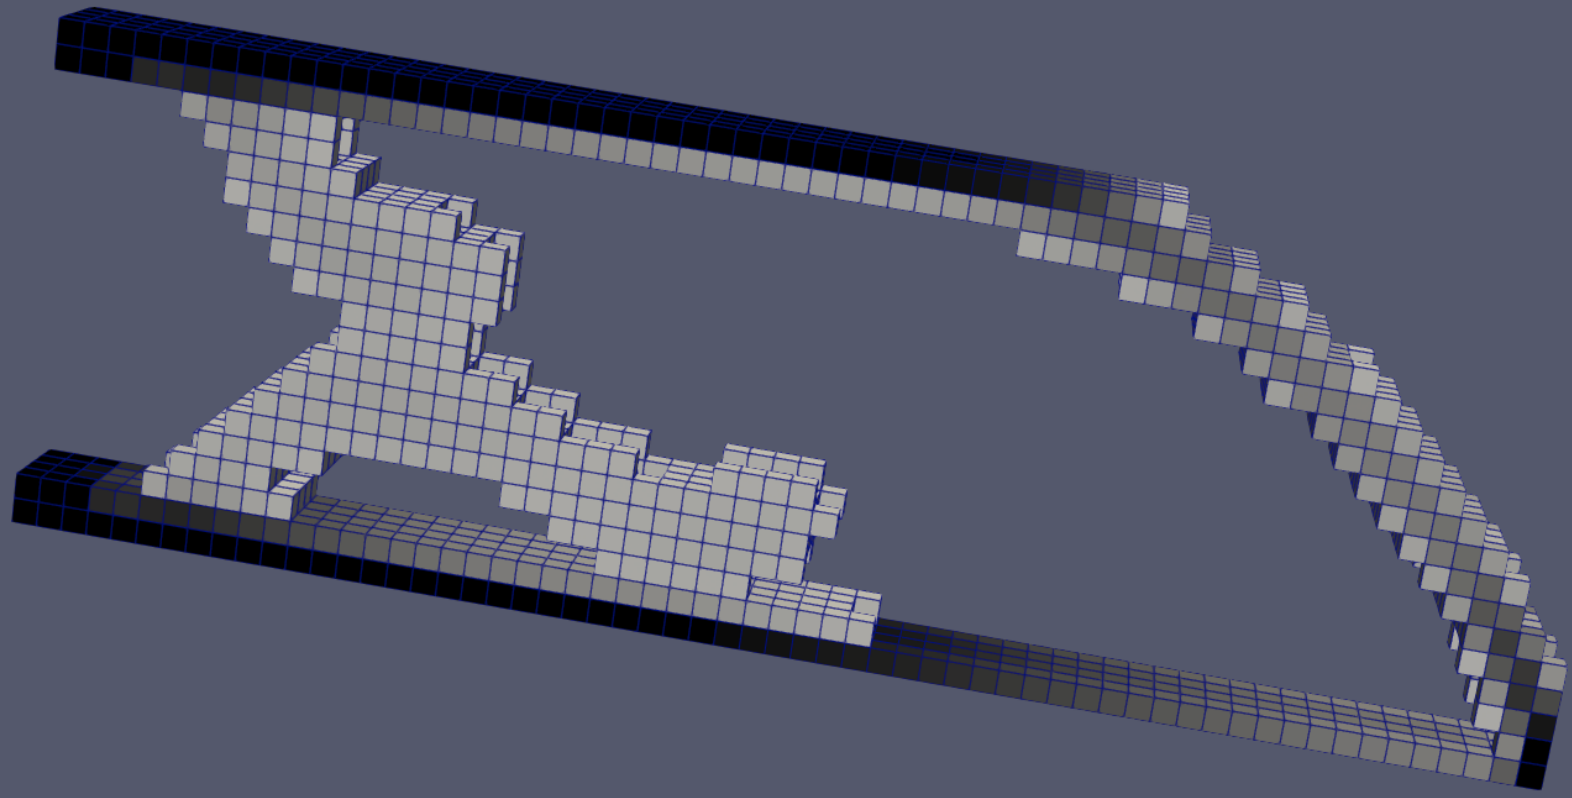
\includegraphics[width=0.32\textwidth]{figures/cantilever_3d_1_auto.png}
		\label{fig:canti3d_1_auto}
	}
	\subfloat[$c(\rho)=2122.6707,~v(\rho)=0.3000$]{
		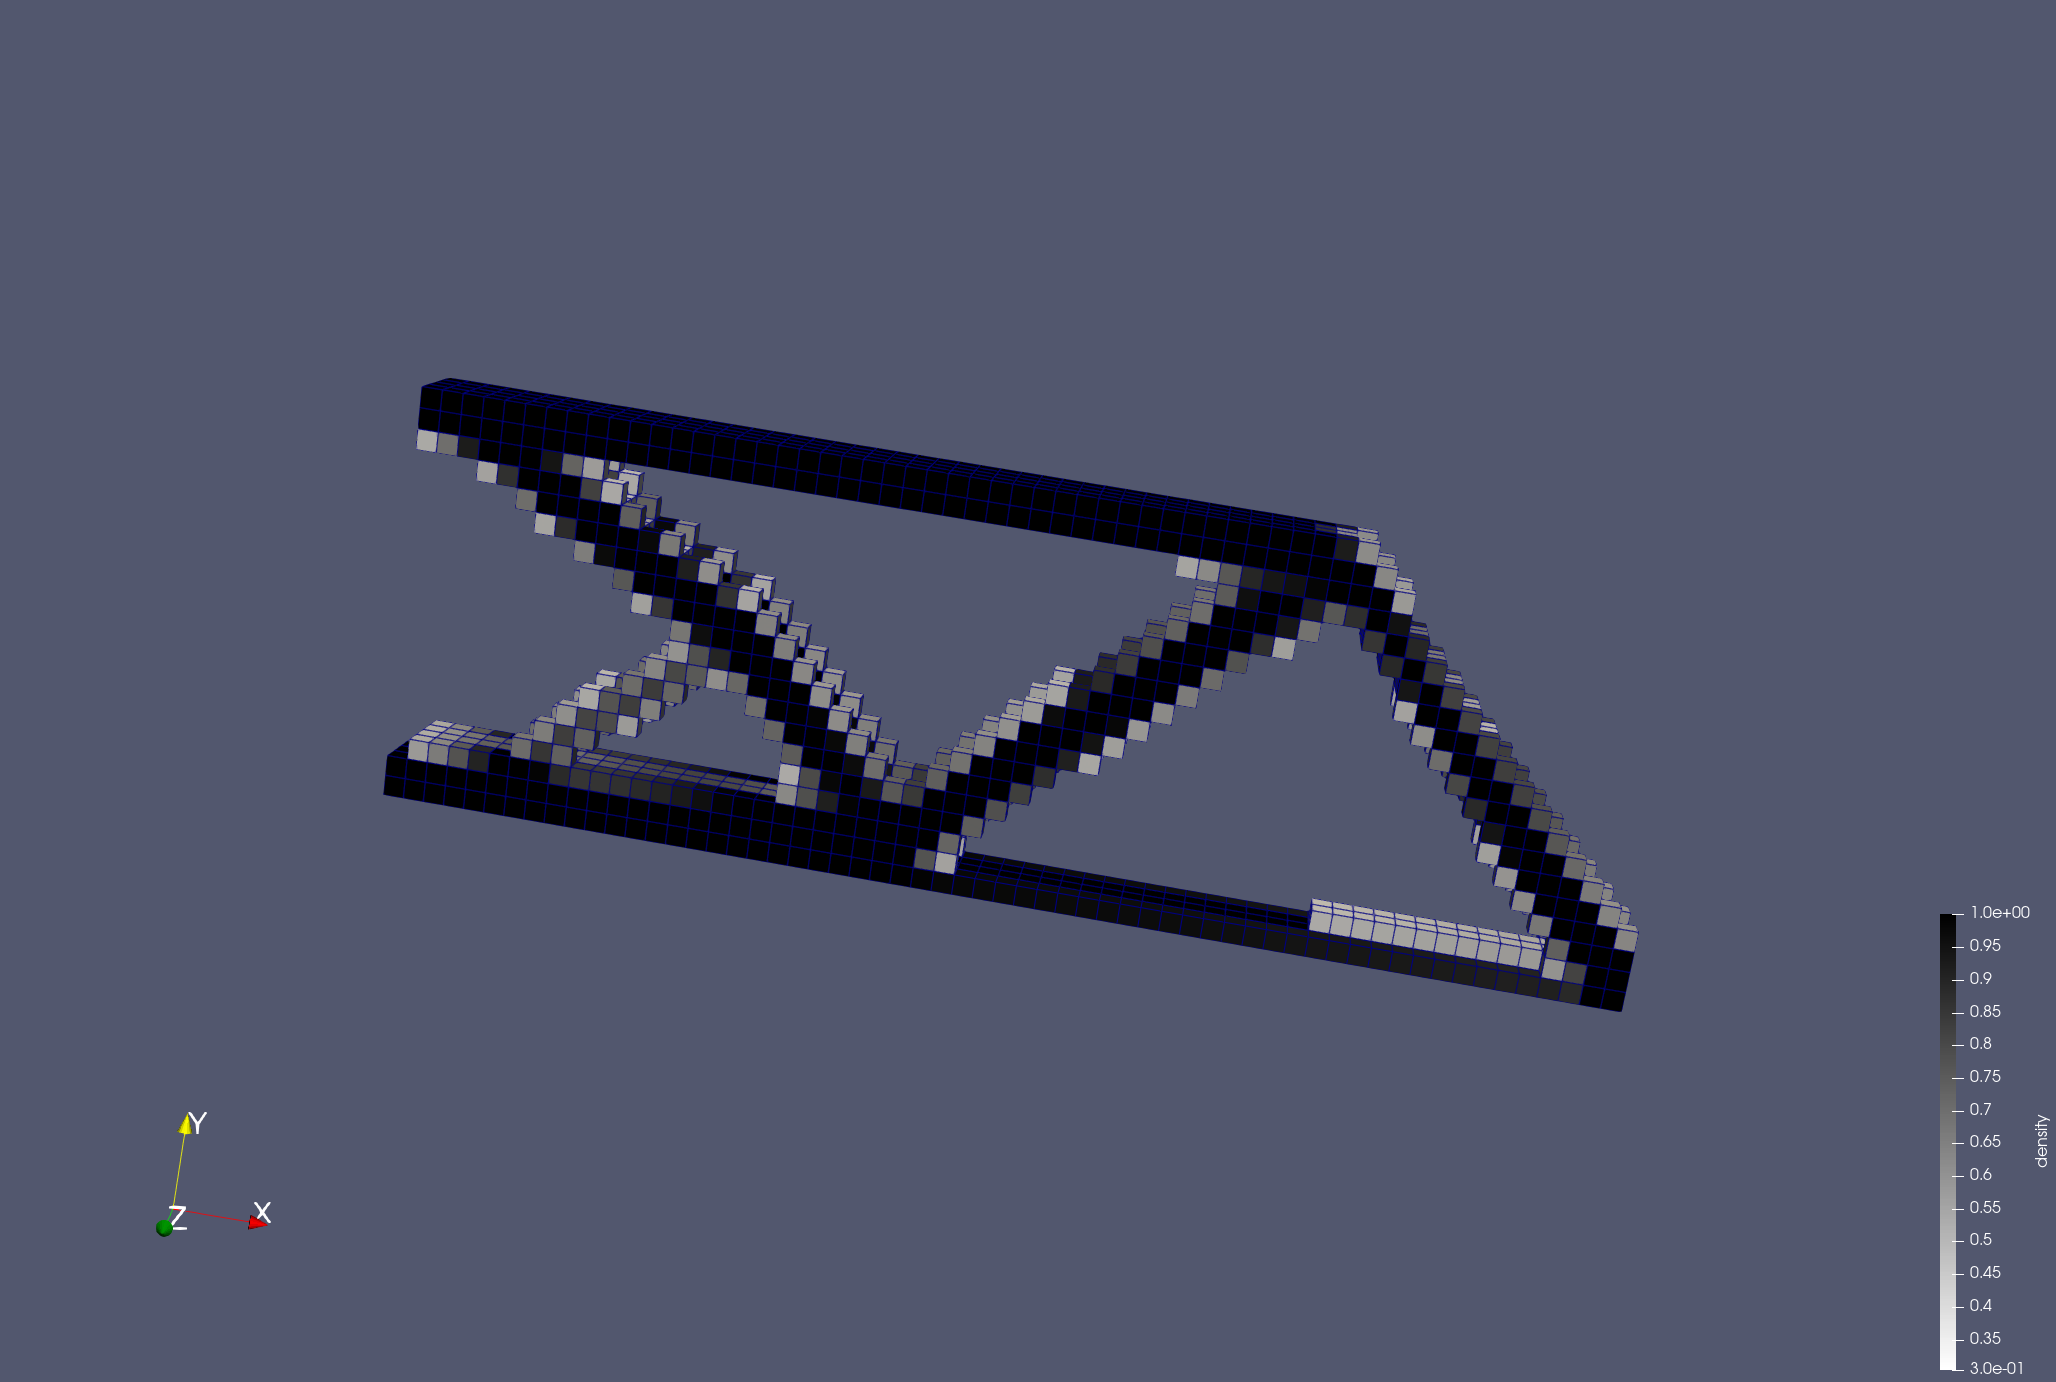
\includegraphics[width=0.32\textwidth]{figures/cantilever_3d_2_auto.png}
		\label{fig:canti3d_2_auto}
	}
	\subfloat[$c(\rho)=2063.5625,~v(\rho)=0.2999$]{
		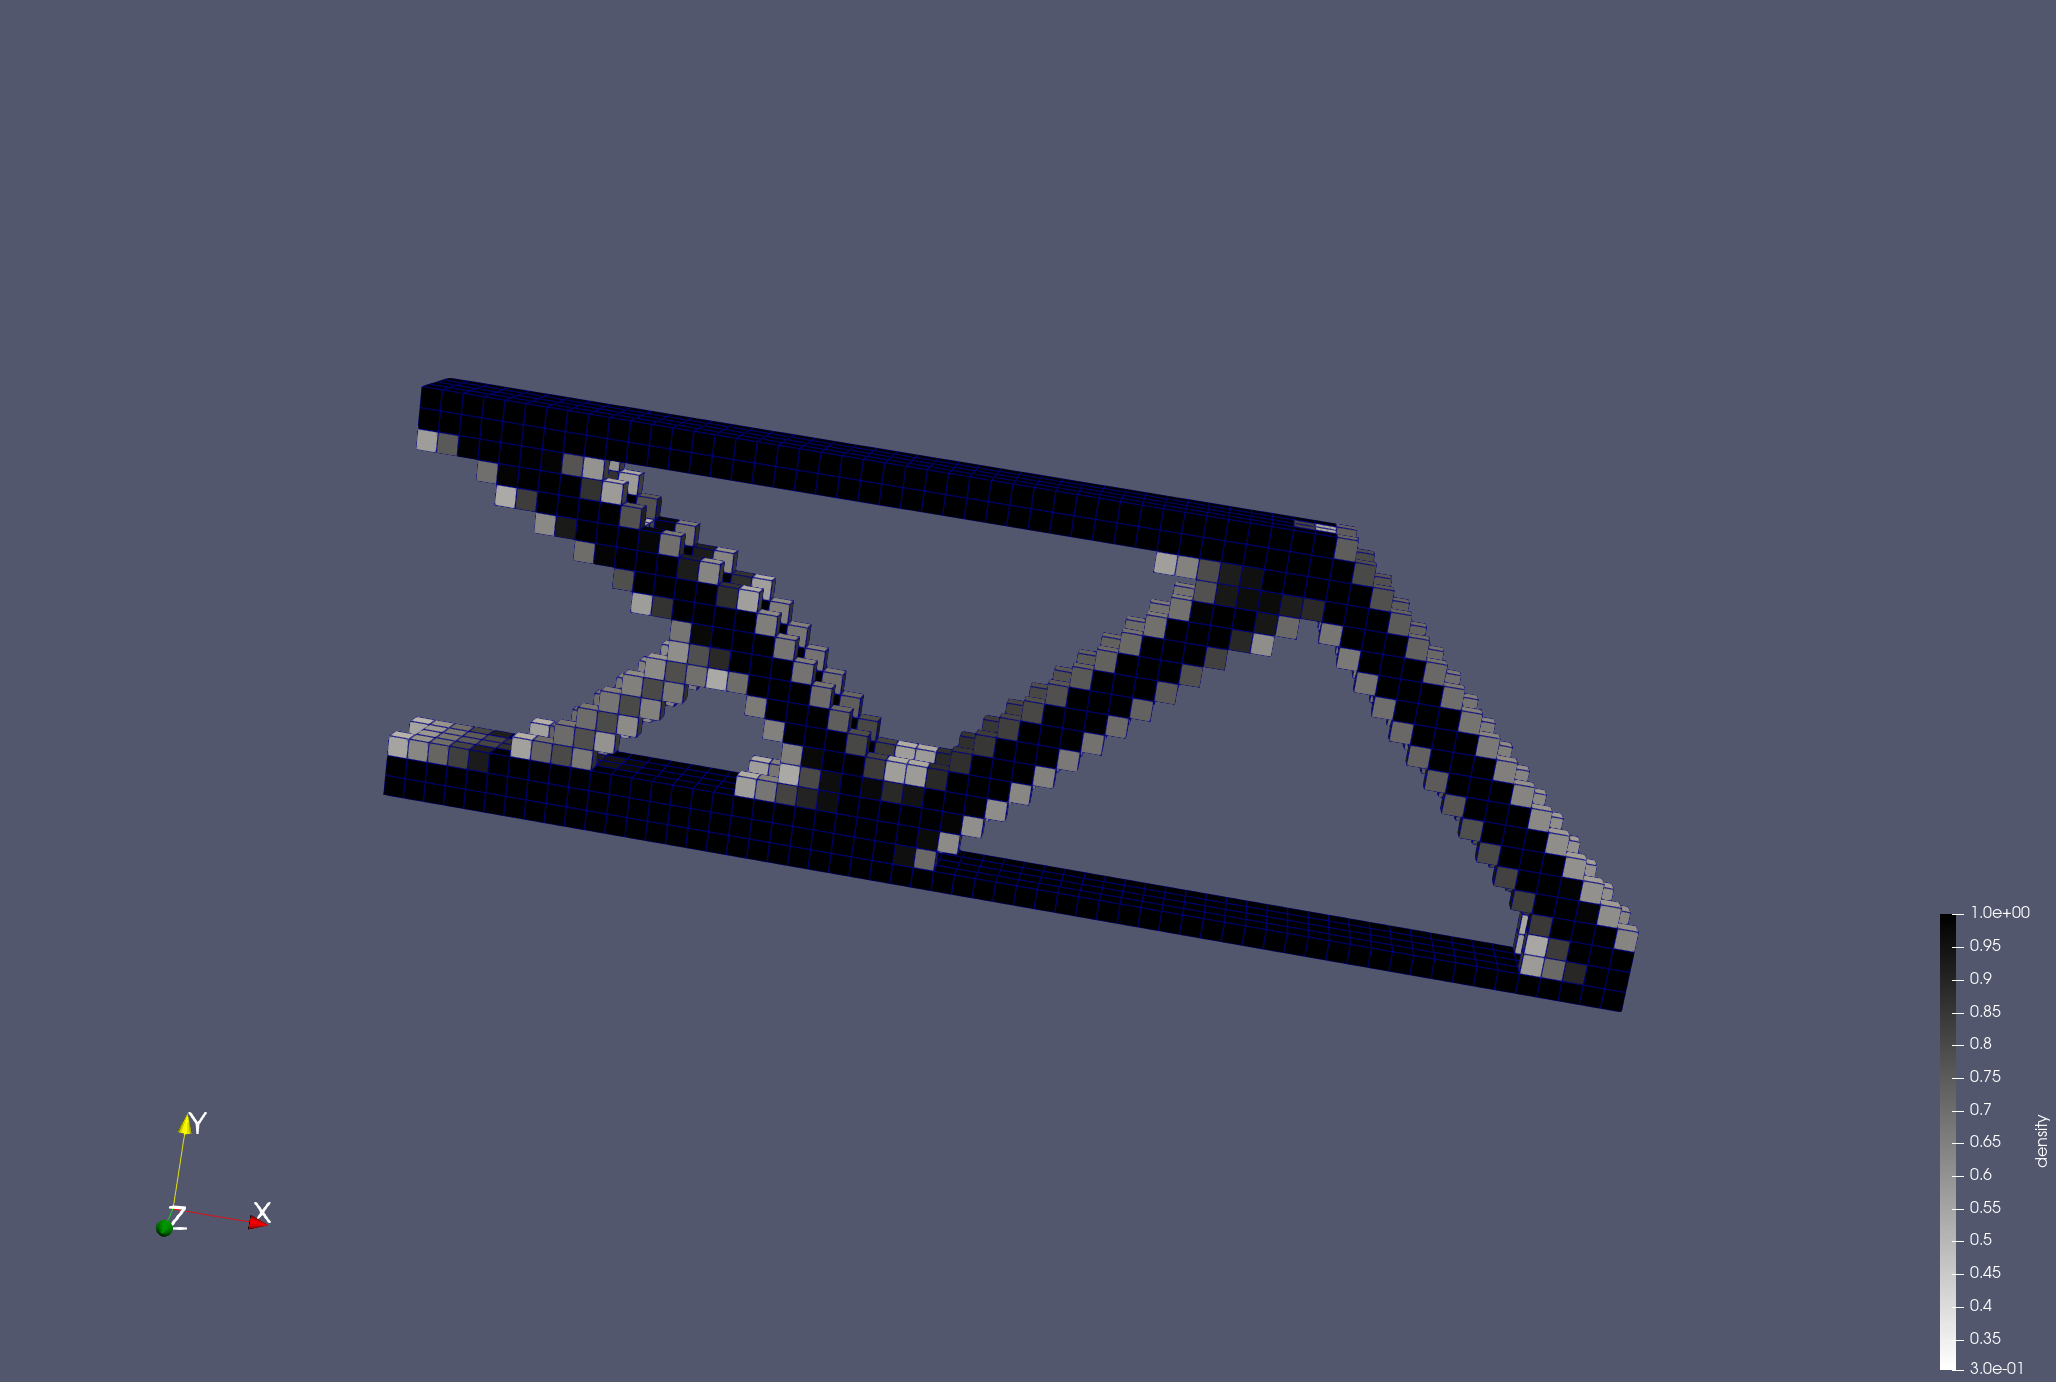
\includegraphics[width=0.32\textwidth]{figures/cantilever_3d_3_auto.png}
		\label{fig:canti3d_3_auto}
	}
	\caption{Topology layouts at iterations 7, 21, and 54 during the 3D cantilever beam optimization using AD. Only elements with $\rho>0.3$ are visualized. Each subfigure also reports the compliance and volume fraction.}
	\label{fig:canti3d_ad_topos}
\end{figure}

As observed from Figure~\ref{fig:canti3d_ad_convergence} and Figure~\ref{fig:canti3d_ad_topos}, the optimization results obtained using AD are fully consistent with those achieved through manual differentiation in Section~\ref{sec:exp_canti3d}. he compliance converges to approximately $2063.5625$ after 54 iterations, and the volume fraction remains stably around $0.3$. These results confirm that AD accurately computes the sensitivities and effectively guides the optimization process.

To evaluate the computational efficiency of AD, we compare the optimization times of AD and manual differentiation under the same 3D cantilever beam problem setting. The results are summarized in Table~\ref{tab:ad_vs_manual}.

\begin{table}[htbp]
	\centering
	%	\setlength{\tabcolsep}{4pt} % 减小列间距
	\caption{Performance comparison of differentiation methods in the 3D cantilever beam optimization problem. All values are reported in seconds.}
	%	\small % 使用小字体
	\begin{tabular}{ccccc}
		\toprule
		\textbf{Differentiation Method} & \textbf{Iterations} & \textbf{Total} & \textbf{1st Iter.} & \textbf{Avg. Iter.} \\
		\midrule
		Manual Differentiation & 54 & 39.562 & 1.940 & 0.710 \\
		AD & 54 & 39.865 & 1.832 & 0.718 \\
		\bottomrule
	\end{tabular}
	\label{tab:ad_vs_manual}
\end{table}

As shown in Table~\ref{tab:ad_vs_manual}, the total optimization time and the average iteration time between manual differentiation and AD are nearly identical. This demonstrates the high efficiency of the AD implementation in SOPTX, which introduces no significant computational overhead while maintaining the same high precision as manual differentiation.

The multi-backend mechanism of SOPTX allows users to flexibly switch between different computational backends. In addition to PyTorch, SOPTX also supports the JAX backend~\cite{bradbury2018jax}, which offers equally powerful AD capabilities. The sensitivity computation code remains identical when using JAX, users simply need to switch to the JAX backend by executing:
\begin{lstlisting}
	bm.set_backend('jax')
\end{lstlisting}

Using AD with the JAX backend, we perform topology optimization for the 3D cantilever beam. The final optimized topology is shown in Figure~\ref{fig:canti3d_ad_jax}.

\begin{figure}[htp] 
	\centering 
	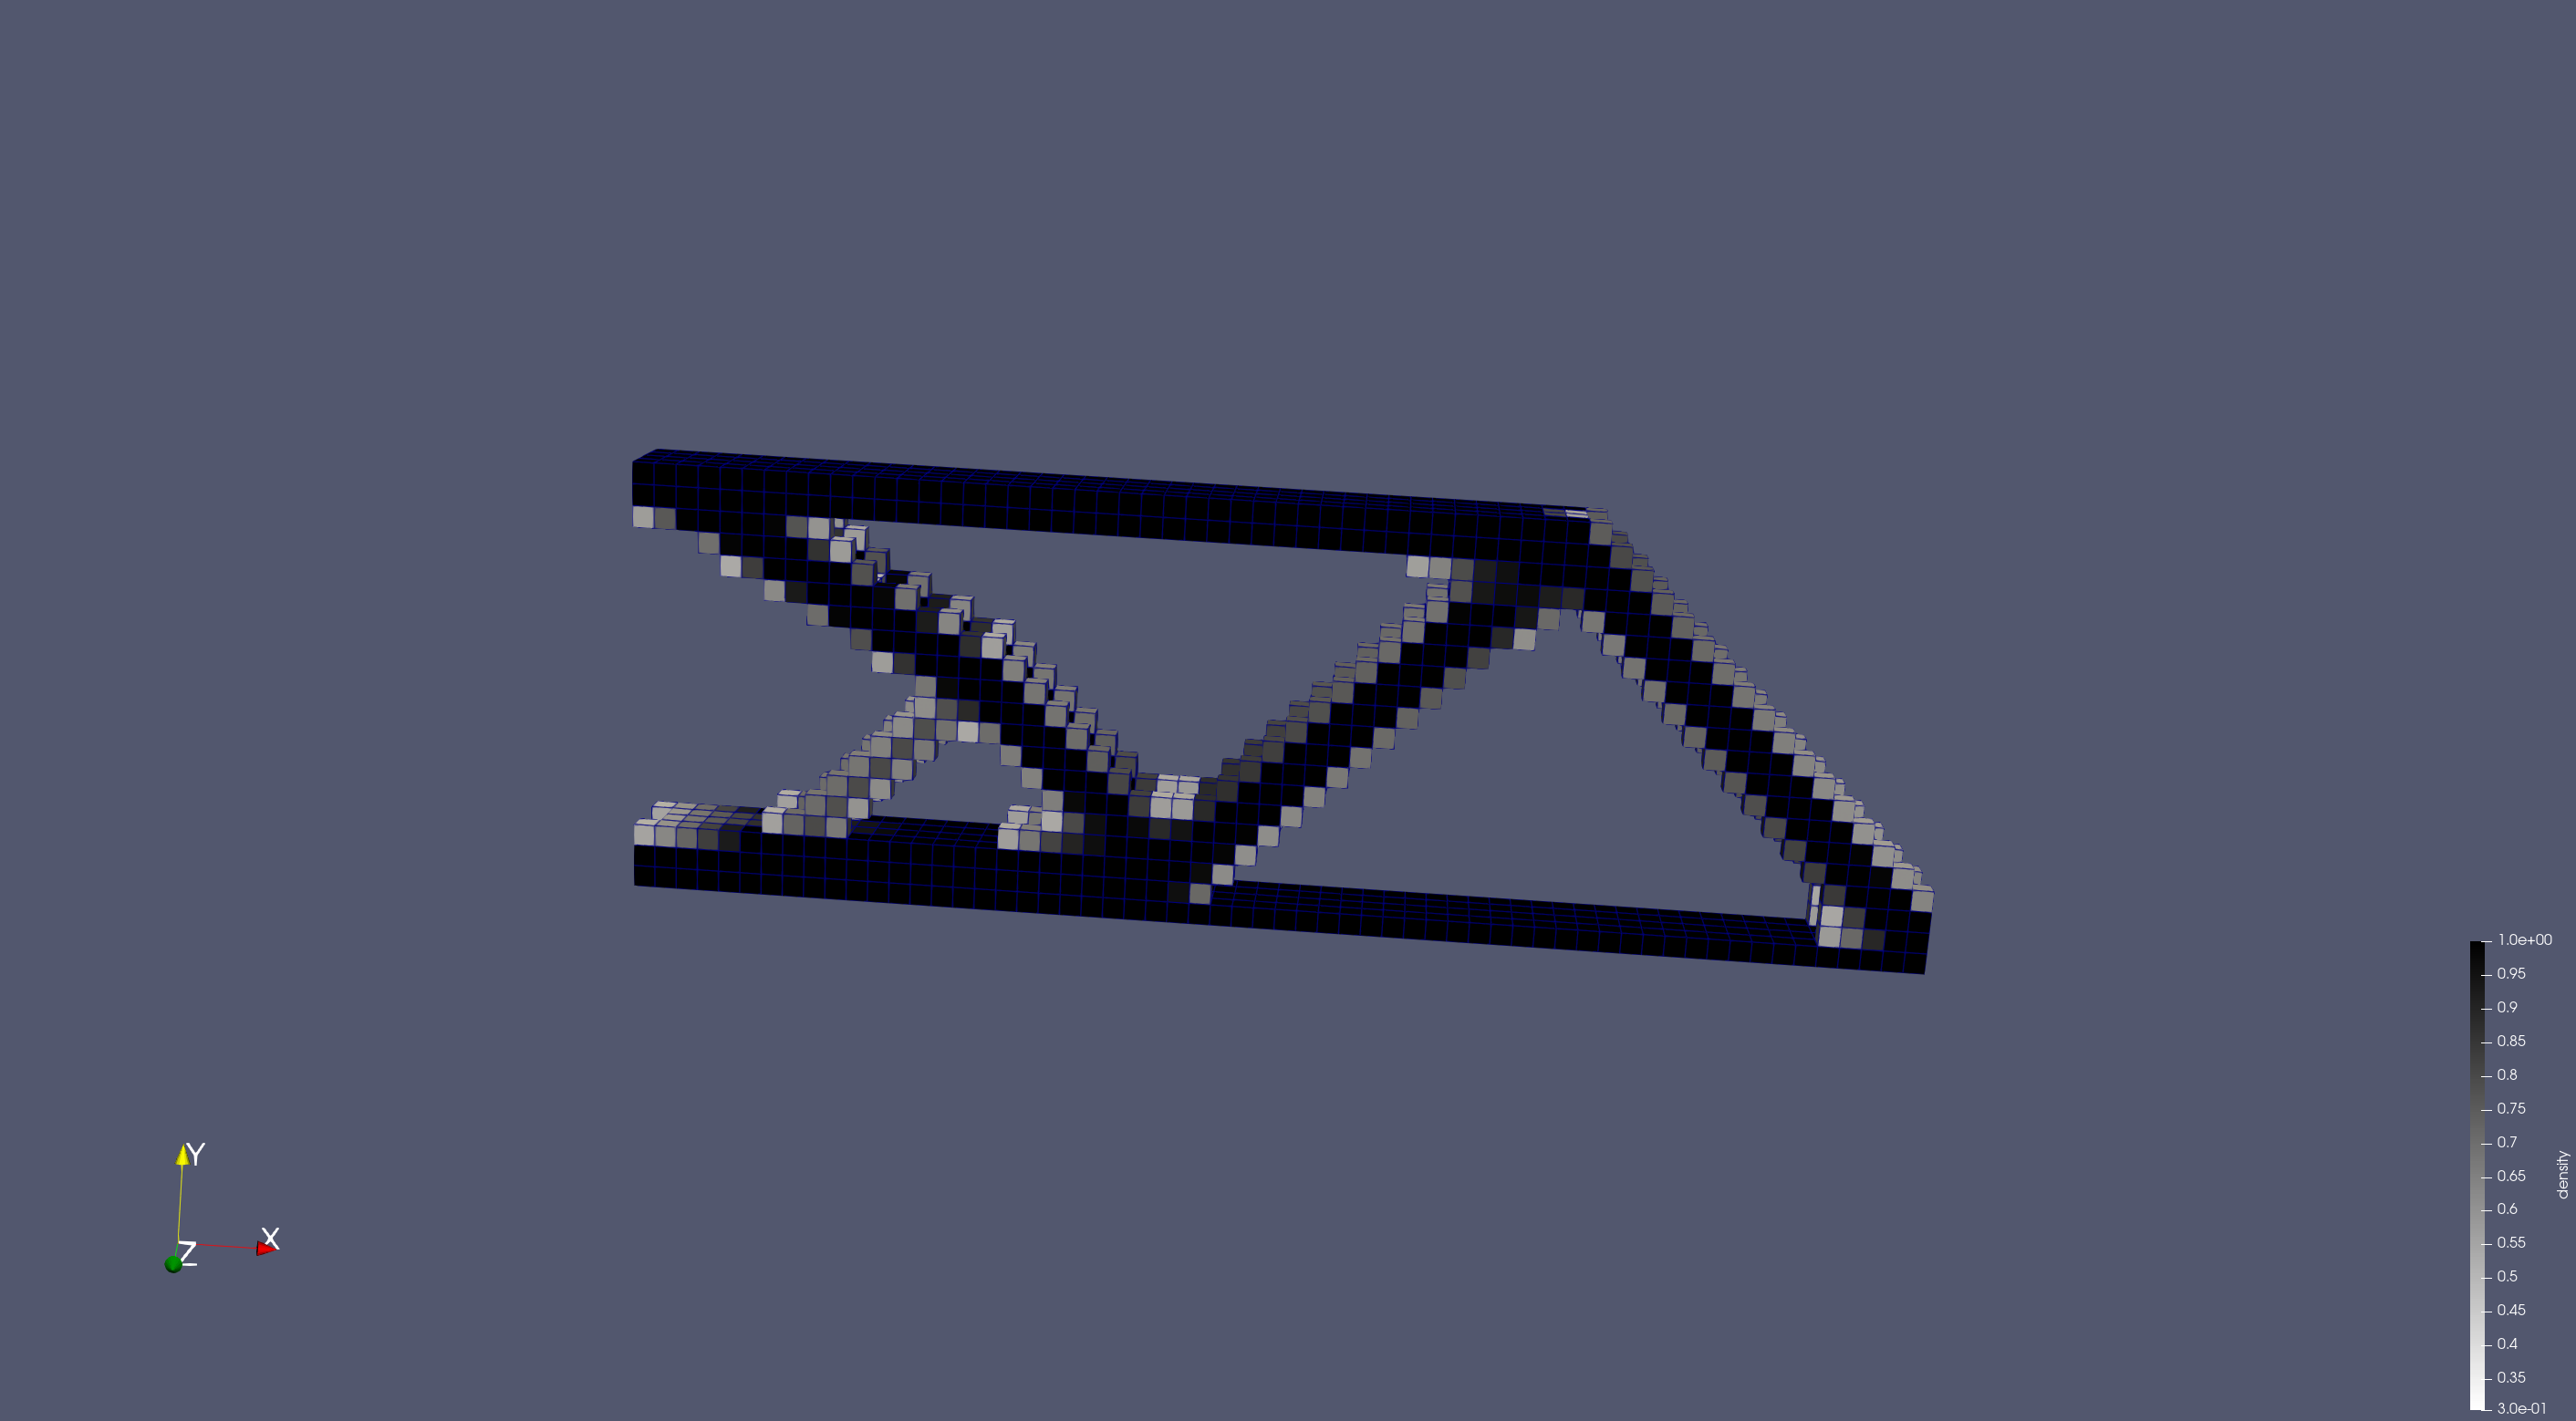
\includegraphics[width=0.8\textwidth]{figures/cantilever_3d_auto_jax.png} \caption{Final optimized topology of the 3D cantilever beam using AD with the JAX backend.} \label{fig:canti3d_ad_jax} 
\end{figure}

It is noteworthy that the final optimization result obtained using JAX is fully consistent with that obtained using PyTorch, demonstrating the stability and feasibility of the SOPTX framework when applying AD across different computational backends.

The application of AD in TO offers several significant advantages:
\begin{itemize} 
	\item \textbf{Simplified Model Switching}: In TO, the choice of material interpolation model directly influences the optimization results. Besides the commonly used SIMP model, alternative models such as RAMP~\cite{stolpe2001alternative} are also widely applied in specific scenarios. With AD, users can easily switch between different interpolation models. For instance, when switching from SIMP to RAMP, the material stiffness gradient can be automatically computed by AD without manually deriving complex formulas. This greatly improves development efficiency and enhances the flexibility of model experimentation.
	\item \textbf{Seamless Constraint Switching}: TO often involves multiple constraints. In addition to volume constraints, manufacturing constraints such as length scale control~\cite{guest2009imposing}, connectivity~\cite{li2016structural}, overhang limitations~\cite{qian2017undercut}, and material usage restrictions~\cite{sanders2018multi} are frequently imposed. Traditionally, adding or modifying constraints requires manually re-deriving sensitivity expressions. By introducing AD, this process becomes fully automated. The system can seamlessly adapt to new constraint settings, significantly improving optimization adaptability and development efficiency.
	\item \textbf{Support for Complex Problems}: For TO problems involving multiphysics coupling, nonlinear materials, or complex geometric constraints, AD efficiently handles the computation of complicated gradients, allowing users to focus on modeling rather than mathematical derivations. Moreover, AD can automatically manage combined sensitivity computations when using techniques like density filtering and Heaviside projection. This capability further enhances the practical applicability and flexibility of the SOPTX framework in complex engineering scenarios.
\end{itemize}

Through the optimization example of the 3D cantilever beam, this section has demonstrated the powerful potential of AD within the SOPTX framework. Numerical results show that AD achieves comparable precision and computational efficiency to traditional manual differentiation methods without introducing any significant overhead. The multi-backend support of SOPTX, including PyTorch and JAX, further enhances the flexibility and scalability of the framework. The application of AD not only simplifies sensitivity analysis but also facilitates the exploration of novel material models and constraint conditions. These features make SOPTX a valuable tool in the field of topology optimization, providing robust support for education, research, and engineering applications.

\subsection{Multi-Backend Switching}\label{sec:exp_multi_backend}
The SOPTX framework supports multi-backend switching, currently offering three computational backends: NumPy, PyTorch, and JAX. Backend switching is managed through the \textit{Tensor Backend Manager}, and users can easily switch between different backends by using the \texttt{set\_backend} function:
\begin{lstlisting}
	bm.set_backend('numpy')    
	bm.set_backend('pytorch') 
	bm.set_backend('jax')     
\end{lstlisting}

To verify the consistency and reliability of SOPTX across different computational backends, we conduct tests on the 3D cantilever beam optimization problem described in Sections~\ref{sec:exp_canti3d} and~\ref{sec:exp_canti3d_ad}, using identical parameter settings. The problem is solved separately under the NumPy, PyTorch, and JAX backends. The optimization results show that the convergence histories and final topology layouts are highly consistent across all three backends:

\begin{figure}[htp]
	\centering
	\subfloat[$c(\rho)=2063.5625,~v(\rho)=0.2999$]{
		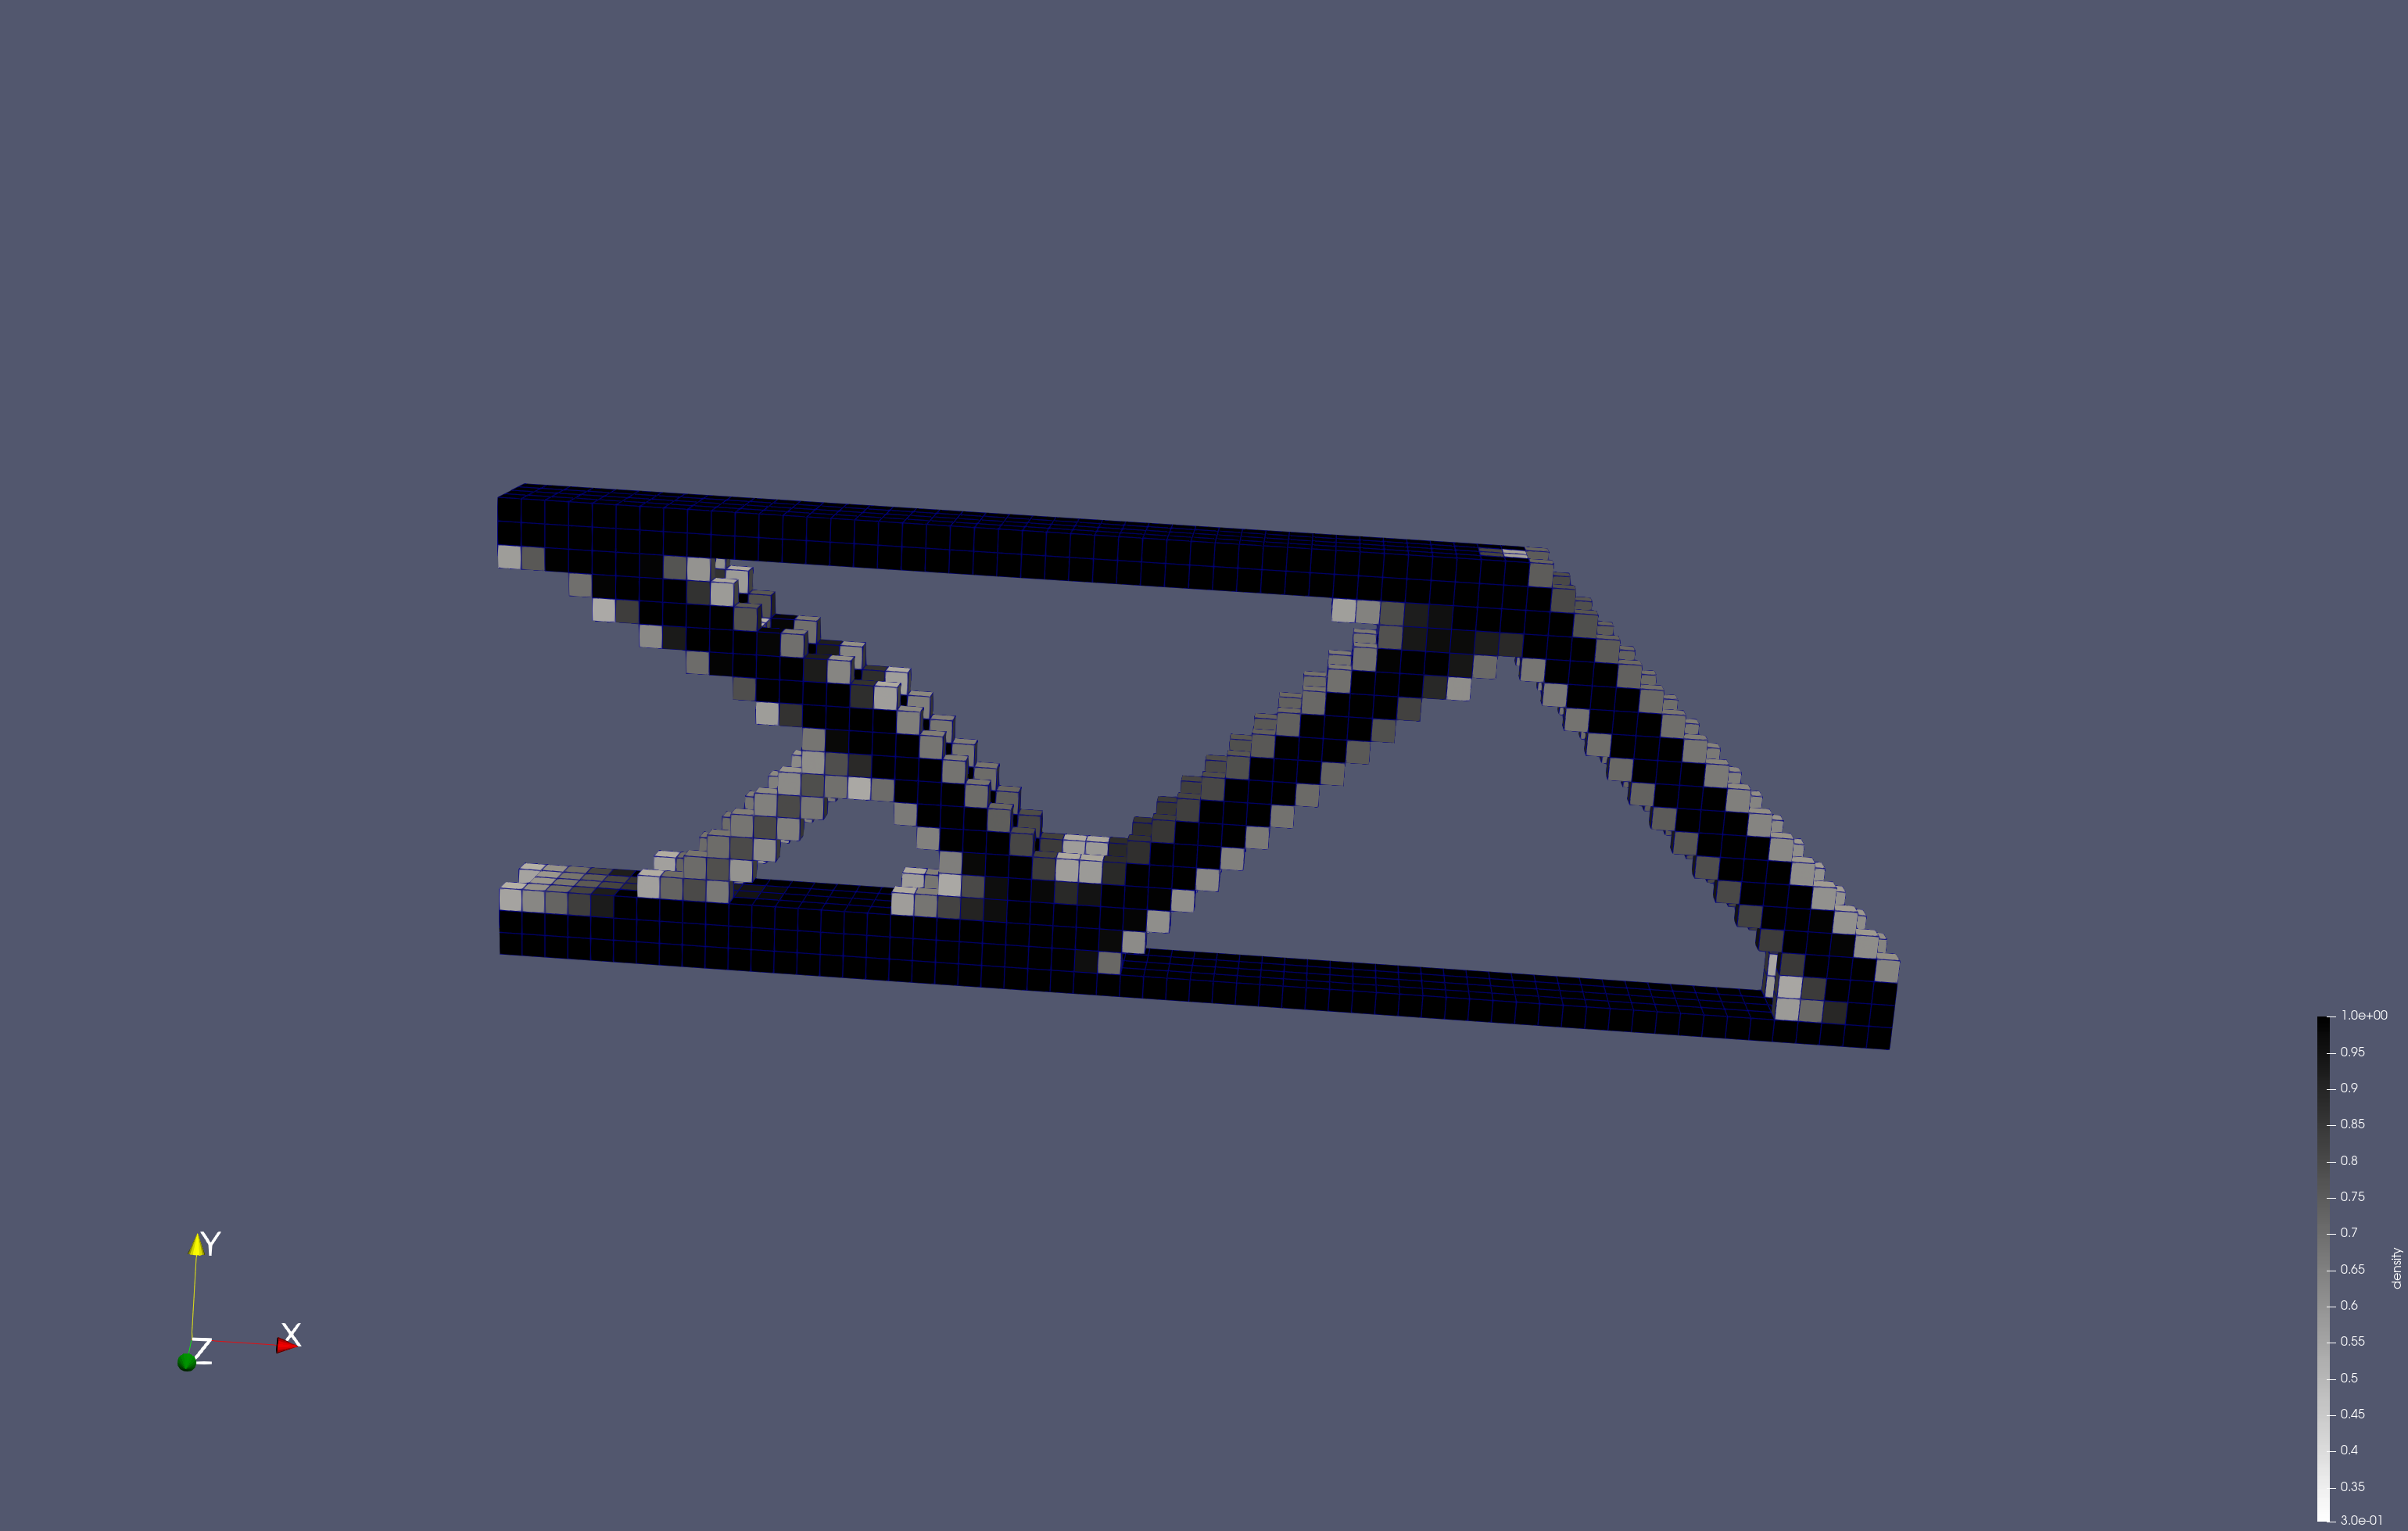
\includegraphics[width=0.32\textwidth]{figures/cantilever_3d_np.png}
		\label{fig:canti3d_np}
	}
	\subfloat[$c(\rho)=2063.5625,~v(\rho)=0.2999$]{
		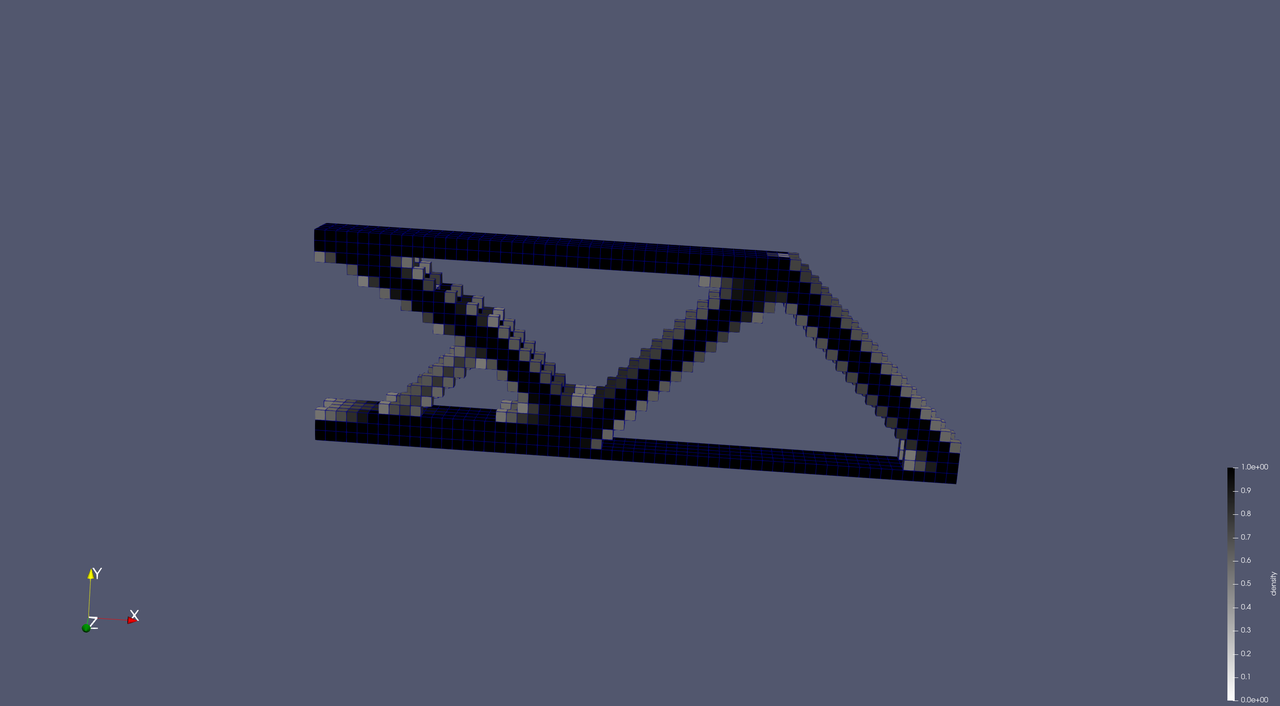
\includegraphics[width=0.32\textwidth]{figures/cantilever_3d_torch.png}
		\label{fig:canti3d_torch}
	}
	\subfloat[$c(\rho)=2063.5625,~v(\rho)=0.2999$]{
		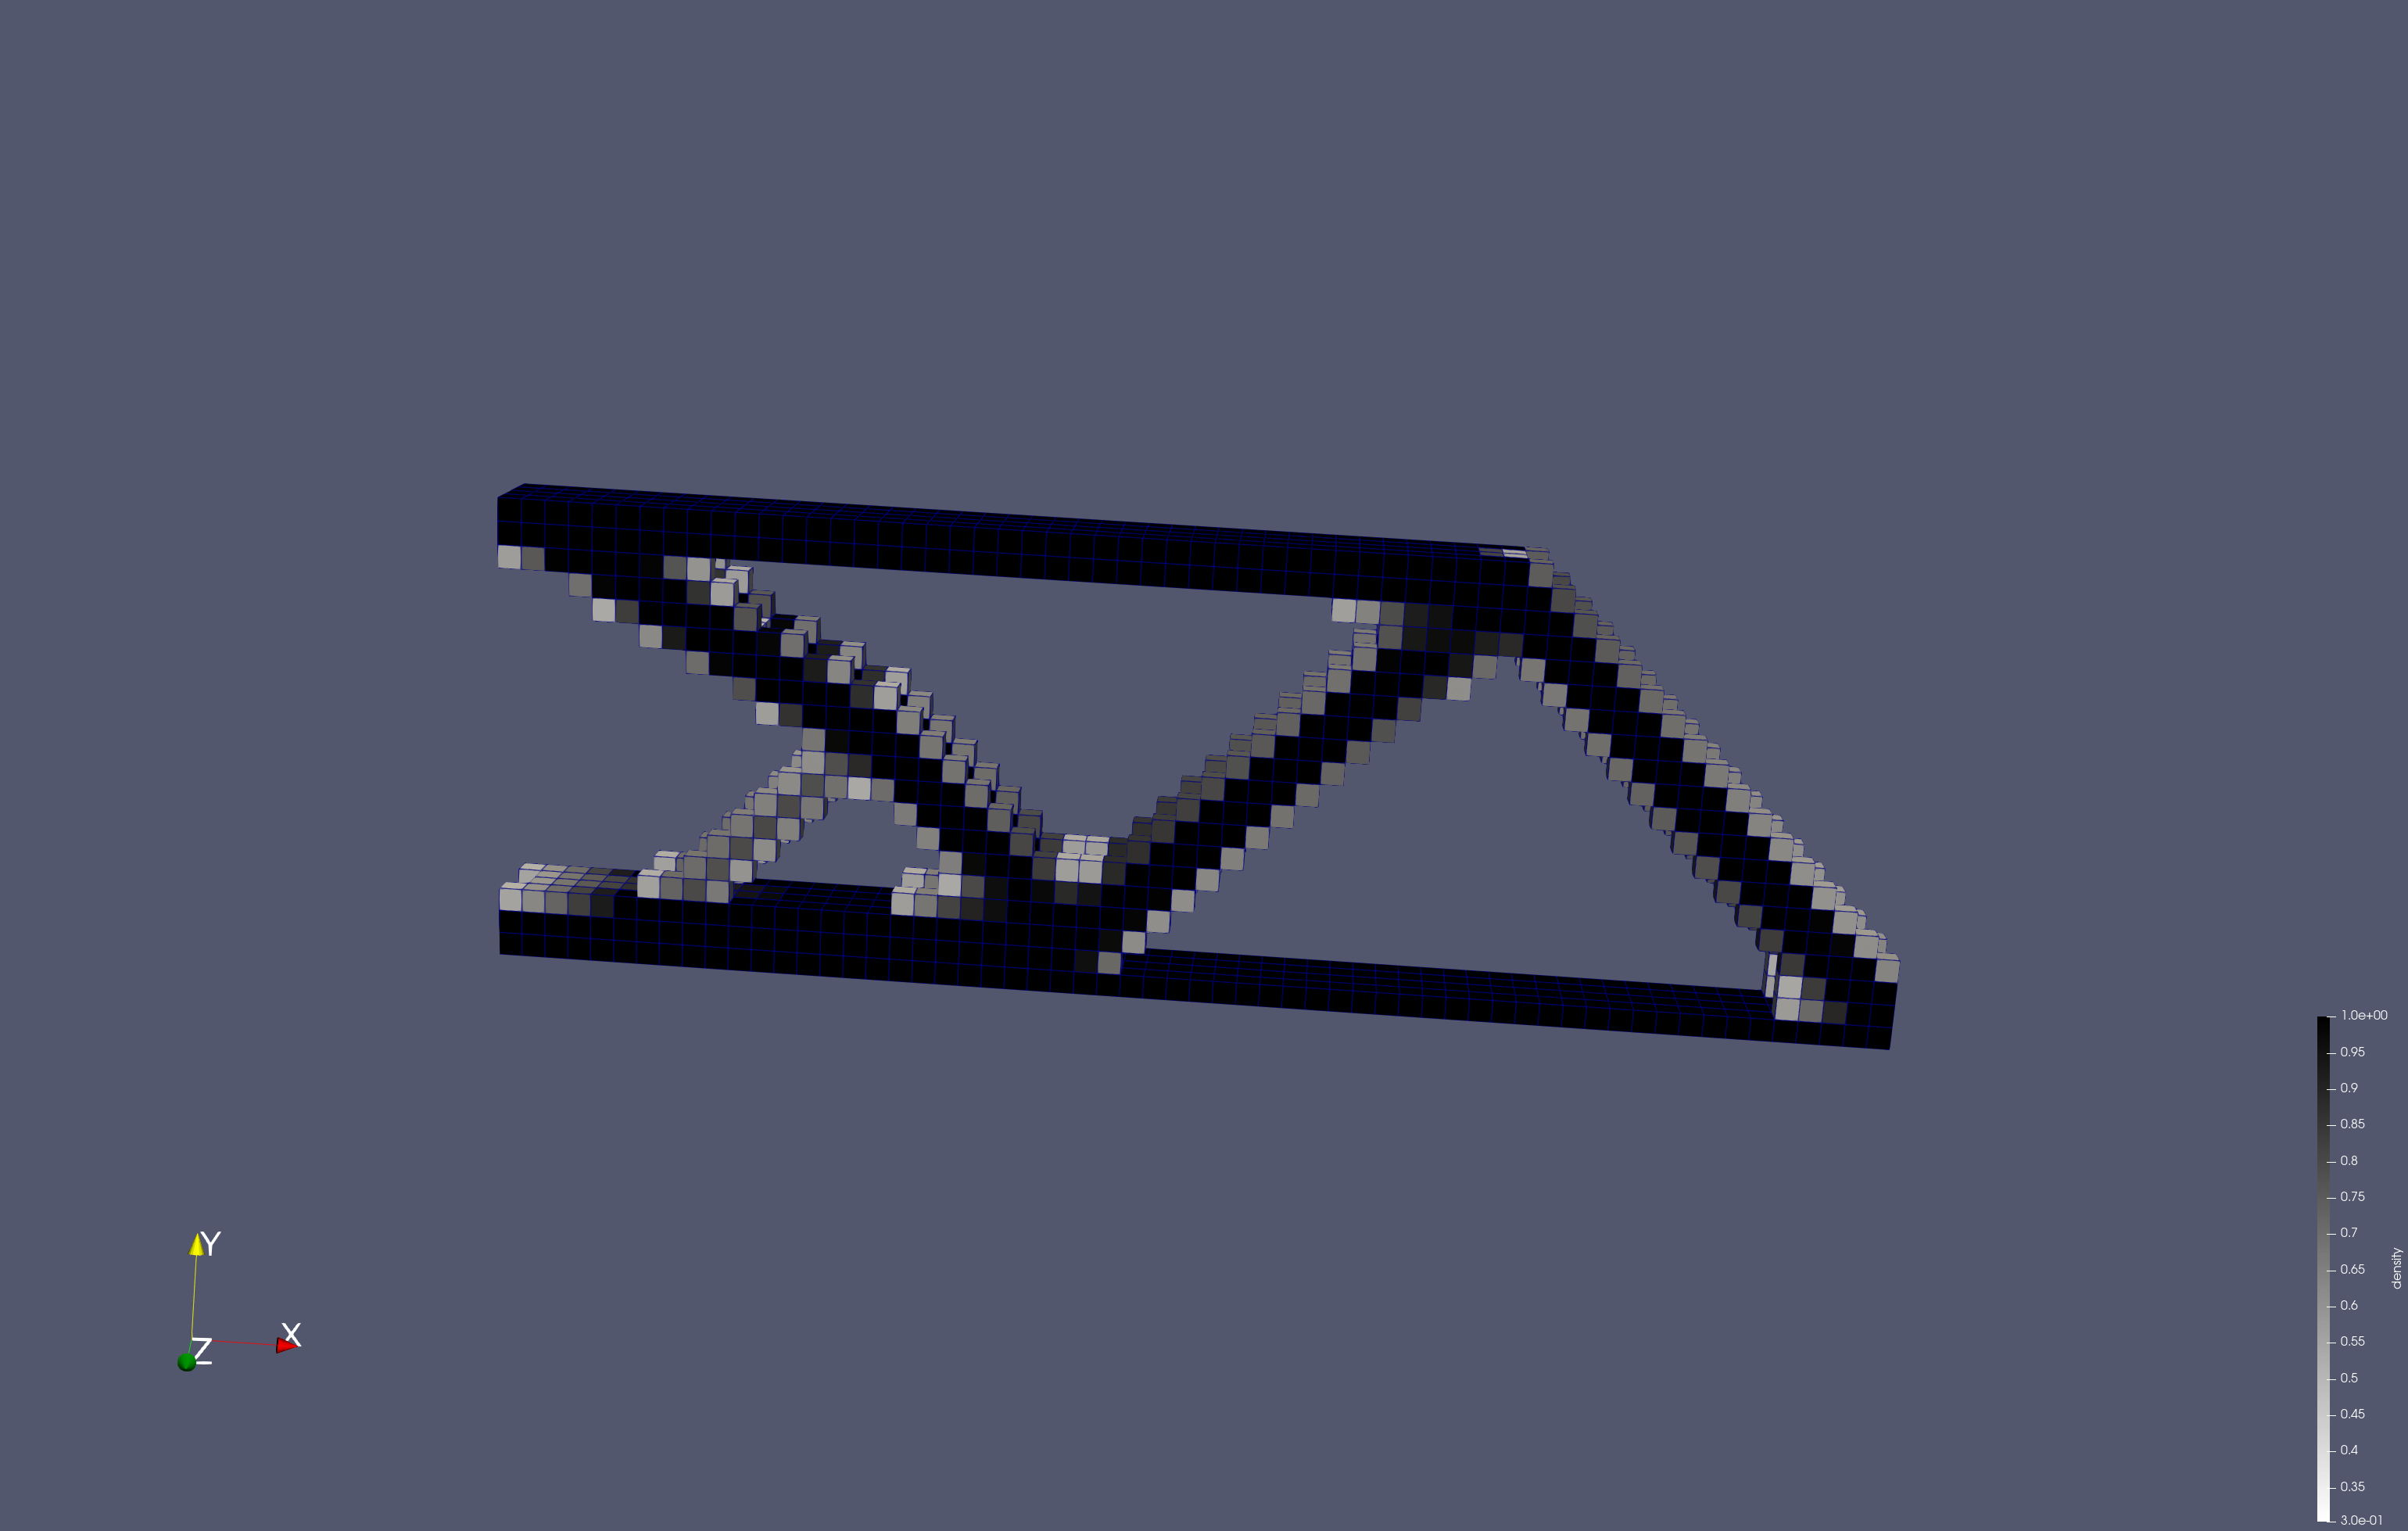
\includegraphics[width=0.32\textwidth]{figures/cantilever_3d_jax.png}
		\label{fig:canti3d_jax}
	}
	\caption{Final optimized topologies of the 3D cantilever beam using three different backends (elements with $\rho>0.3$ are visualized). Left: NumPy backend; Middle: PyTorch backend; Right: JAX backend.}
	\label{fig:canti3d_backend_compare}
\end{figure}

As shown in Figure~\ref{fig:canti3d_backend_compare}, after 54 iterations, the compliance in all three backends converges to approximately $2063.5625$, and the volume fraction stabilizes around $0.3$. The final topology layouts are nearly identical. This consistency highlights the effectiveness of SOPTX's unified numerical abstraction and rigorous testing strategy, ensuring the reliability and stability of the algorithms across different computational backends.

In addition to multi-backend switching, SOPTX also supports computations on GPUs to further enhance computational efficiency, especially when solving large-scale 3D TO problems. By default, all computations are performed on the CPU (\texttt{device='cpu'}). However, users can migrate computations to the GPU (e.g., CUDA devices) through two methods:
\begin{enumerate}
	\item \textbf{Set the Default Device Globally}: Users can set the default device for all tensors globally by executing:
	\begin{lstlisting}
	bm.set_default_device('cuda')
	\end{lstlisting}
	This method places all subsequently created tensors on the GPU by default, and all associated computations, such as matrix assembly and linear solving, are performed on the GPU.
	\item \textbf{Specify the Device When Creating the Mesh}: Alternatively, users can specify the device during mesh initialization:
	\begin{lstlisting}
	mesh = UniformMesh3d(extent=extent, h=h, origin=origin, device='cuda')
	\end{lstlisting}
	By specifying \texttt{device='cuda'} during mesh creation, all computations related to that mesh are performed on the GPU. This approach offers greater flexibility, allowing users to mix CPU and GPU computations within the same program if needed.
\end{enumerate}

\begin{figure}[htp]
	\centering
	\subfloat[$c(\rho)=2063.5625,~v(\rho)=0.2999$]{
		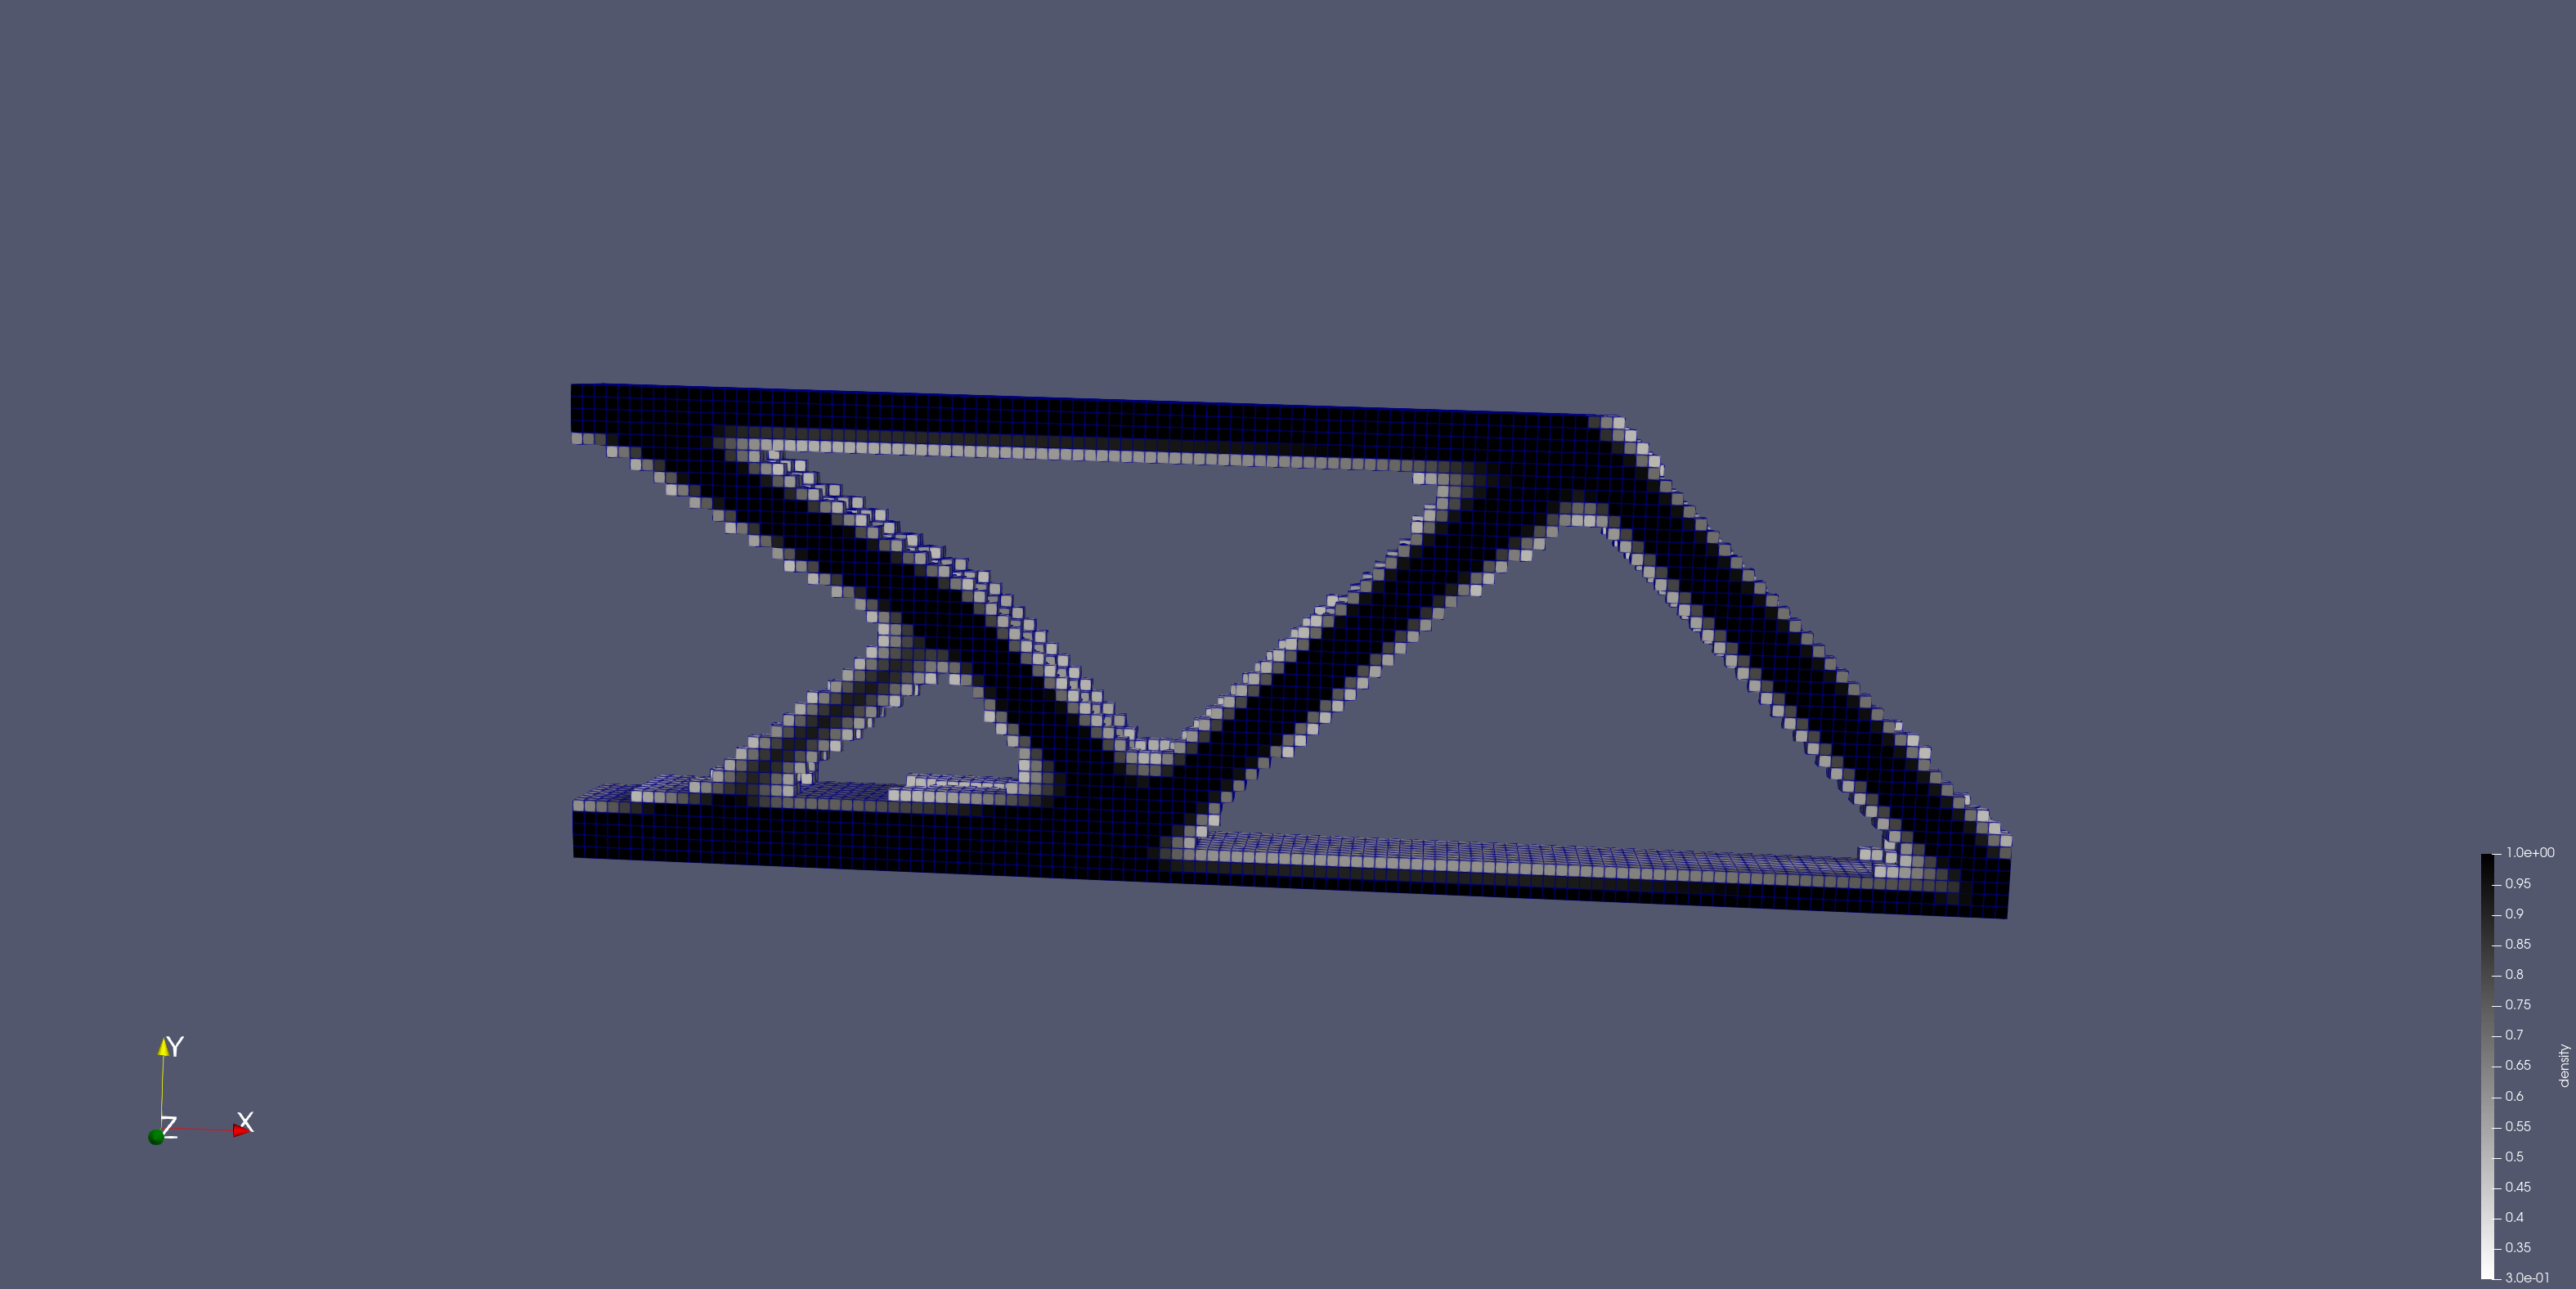
\includegraphics[width=0.5\textwidth]{figures/cantilever_3d_cpu.png}
		\label{fig:canti3d_np}
	}
	\subfloat[$c(\rho)=2063.5625,~v(\rho)=0.2999$]{
		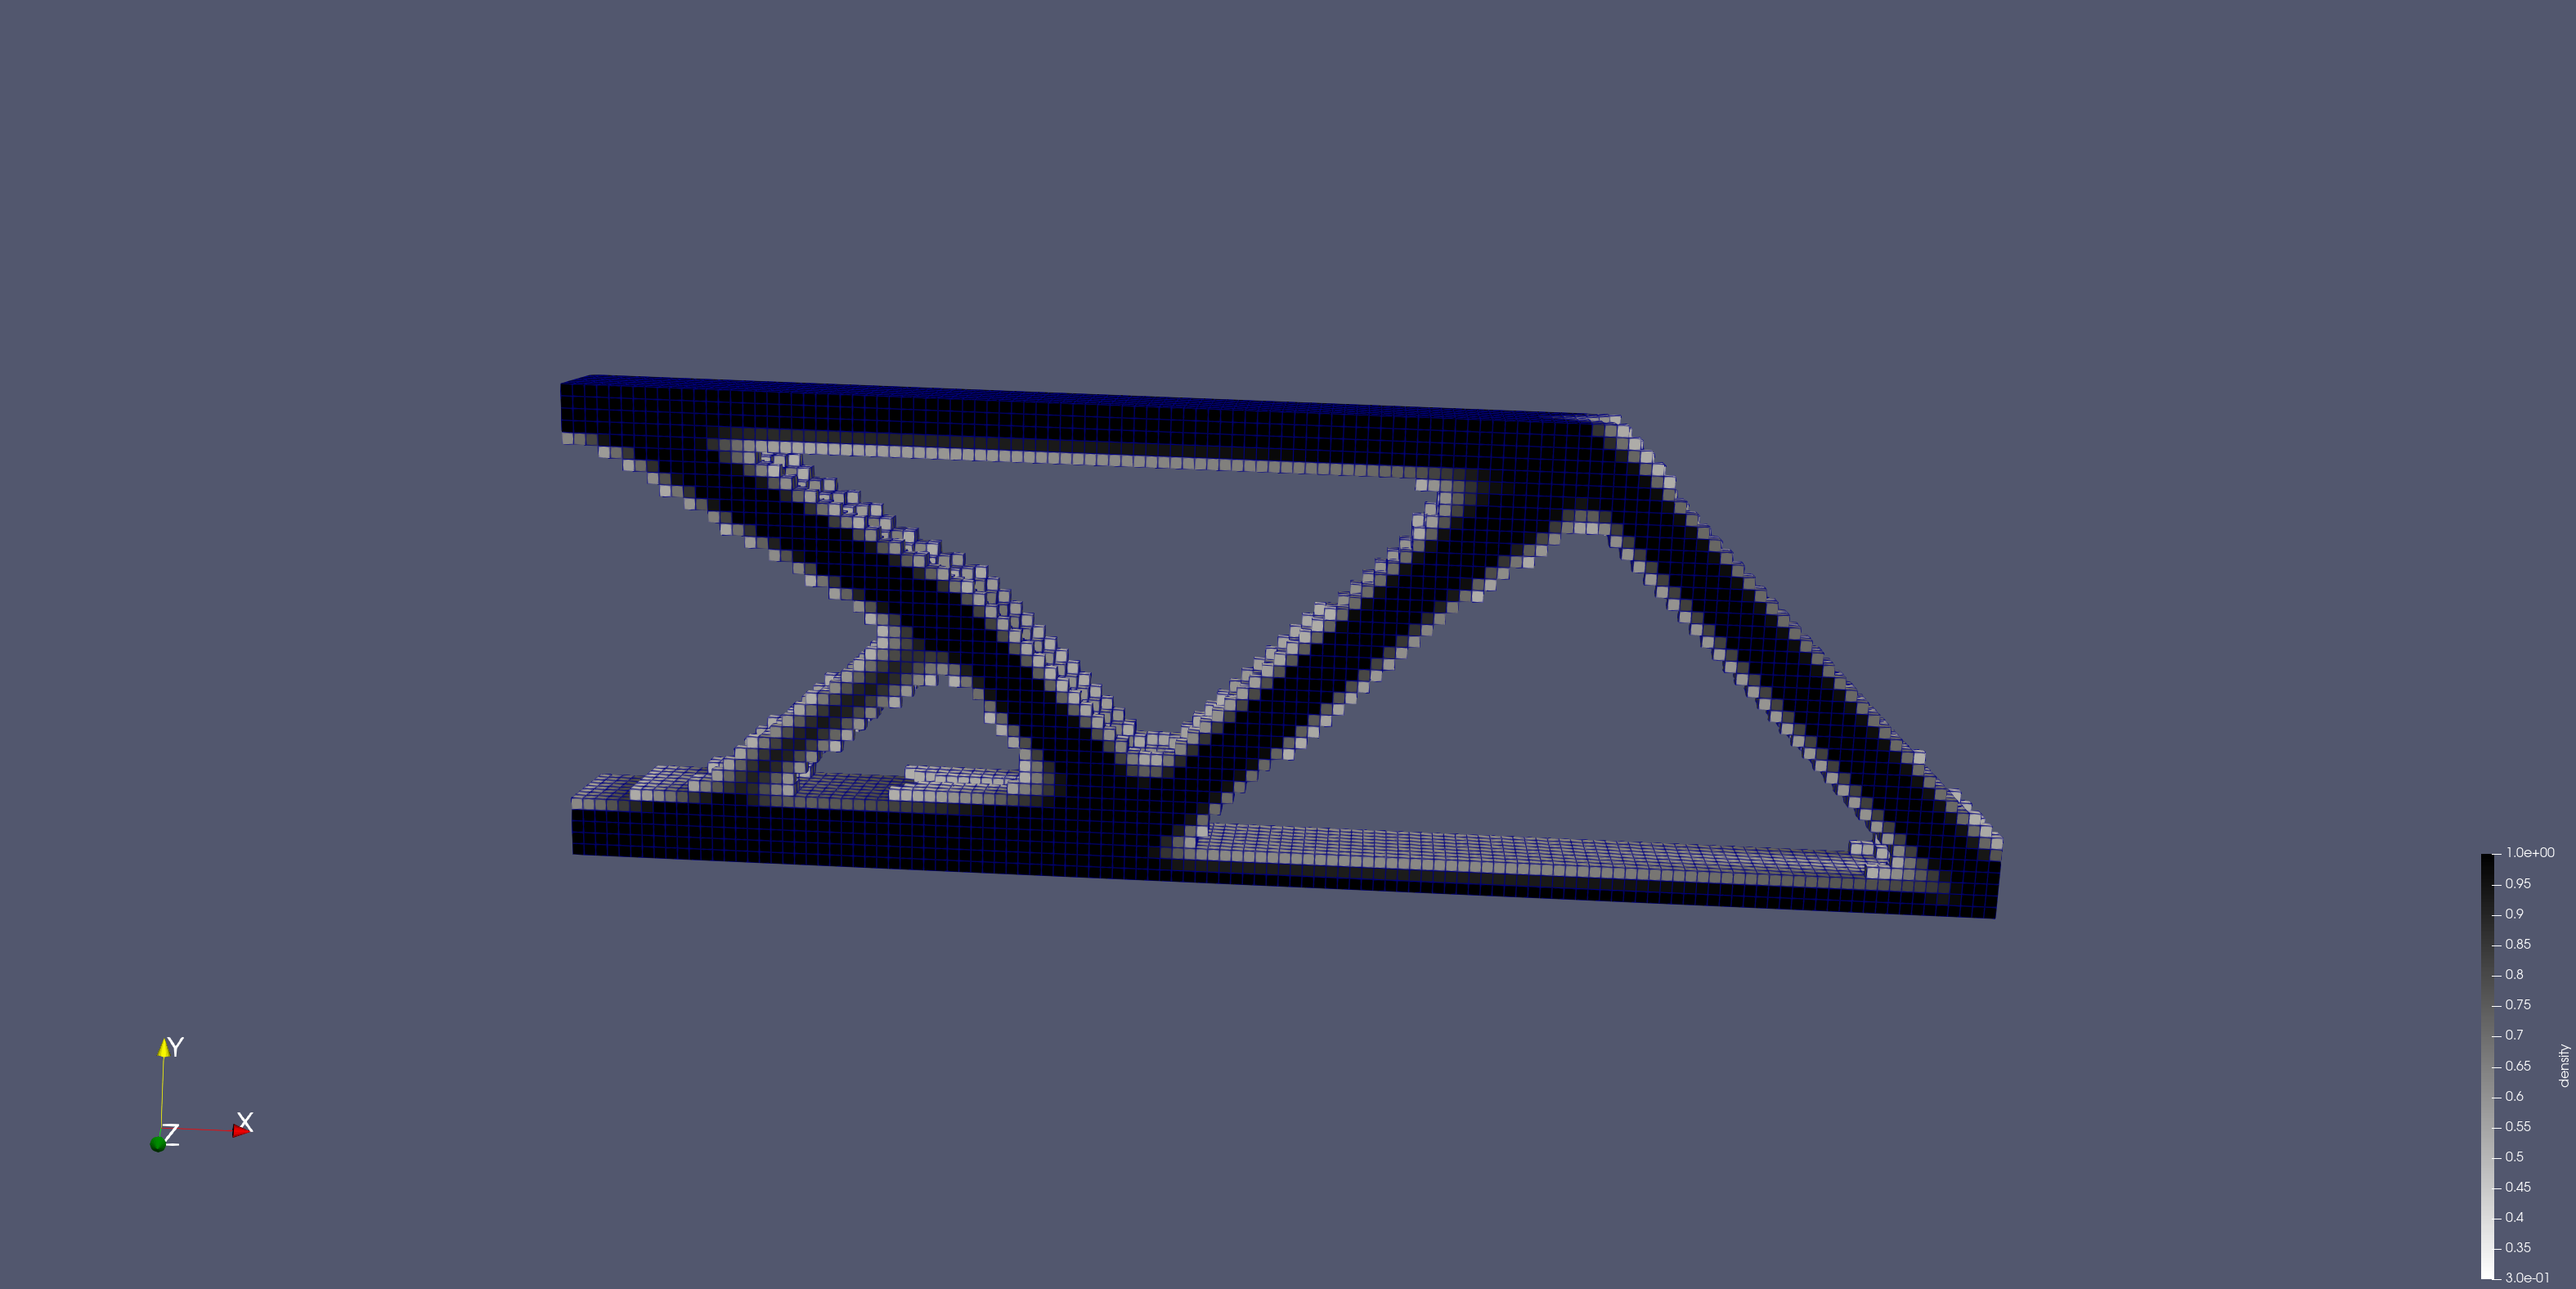
\includegraphics[width=0.5\textwidth]{figures/cantilever_3d_gpu.png}
		\label{fig:canti3d_torch}
	}
	\caption{Final optimized topologies of the 3D cantilever beam using three different backends (elements with $\rho>0.3$ are visualized). Left: NumPy backend; Middle: PyTorch backend; Right: JAX backend.}
	\label{fig:canti3d_backend_compare}
\end{figure}

\section{Conclusion}
This work presents SOPTX, a high-performance topology optimization (TO) framework based on FEALPy. A series of classical benchmark examples have been conducted to validate the effectiveness and practicality of SOPTX in solving TO problems. The development of SOPTX is entirely based on the open-source software FEALPy, without relying on any commercial software. This fully open-source nature not only lowers the technical barrier but also enables users to easily access, learn, and utilize the framework, making it particularly suitable for academic research and educational purposes.

The core innovations of SOPTX are reflected in the following three aspects:
\begin{enumerate} 
	\item \textbf{Modular Design Framework}: Through a loosely coupled architecture, SOPTX supports topology optimization problems in both two and three dimensions, as well as various mesh types (structured and unstructured). It provides a rich library of combinable components, enabling users to flexibly configure and extend the optimization workflow.
	\item \textbf{Cross-Platform Multi-Backend Support and Automatic Differentiation}: Numerical results show that GPU computations take only approximately $33\%$ of the CPU time. Leveraging AD, SOPTX enables the automatic computation of gradients for objective and constraint functions, simplifying sensitivity analysis, reducing development difficulty, and improving computational accuracy.
	\item \textbf{Fast Matrix Assembly Technique}: By optimizing the matrix assembly process, reducing redundant computations, and exploiting matrix sparsity, SOPTX significantly improves finite element matrix assembly efficiency. Benchmark results demonstrate that the average assembly time is reduced from \SI{0.838}{s} to \SI{0.273}{s}, corresponding to approximately $33\%$ of the original method.
\end{enumerate}

Through the example analyses presented in Sections~\ref{sec:exp_mbb_beam} to~\ref{sec:exp_multi_backend}, SOPTX demonstrates outstanding performance in model switching, filter method selection, optimization algorithm flexibility, three-dimensional extension, computational efficiency enhancement, application of automatic differentiation, and multi-backend switching, fully validating its technical advantages.

Although SOPTX currently focuses primarily on density-based TO, it holds promising potential for future development. Leveraging the capabilities of FEALPy in solving heat conduction and Navier–Stokes equations, SOPTX can be extended to optimize thermo-fluid-structure coupling problems, such as thermal protection system designs in aerospace applications or heat dissipation optimization in electronic devices. 

By integrating FEALPy's level set solver module, SOPTX can also support boundary-clear level set methods, enabling the generation of smooth boundaries suitable for precision manufacturing scenarios. In addition, the incorporation of FEALPy's adaptive mesh refinement techniques—particularly local mesh refinement near boundaries---could further enhance the solution accuracy for complex geometries and improve the geometric details of optimized structures. 

Moreover, SOPTX plans to support stress constraints and manufacturing constraints, especially targeting applications in 3D printing and additive manufacturing. Future extensions may include overhang angle control and support structure optimization, aiming to reduce the use of support materials, improve printing efficiency, and meet the high standards of lightweight design and manufacturability required in fields such as aerospace, automotive engineering, and biomedical engineering.

In summary, SOPTX significantly enhances research and development efficiency in the field of TO through its modular design, automatic differentiation capabilities, and multi-backend support. Its open-source nature further lowers the barrier to adoption. Compared to other implementations, SOPTX exhibits notable advantages in computational efficiency, flexibility, and ease of use, providing a solid foundation for both academic research and industrial applications. Looking ahead, SOPTX is expected to play a greater role in multiphysics optimization, lightweight structural design, and additive manufacturing, accelerating the widespread adoption and application of TO in industrial design and manufacturing.

%%%% Acknowledgments %%%%%%%%
\section*{Acknowledgments}
The first and fourth authors were supported by the National Natural Science
Foundation of China (NSFC) (Grant No. 12371410, 12261131501), and the
construction of innovative provinces in Hunan Province (Grant No. 2021GK1010).
The second author was supported by NSF DMS-2012465 and DMS-2309785. The third
author was supported by the National Natural Science Foundation of China (NSFC)
(Grant No. 12171300), and the Natural Science Foundation of Shanghai (Grant No.
21ZR1480500).

\appendix
\renewcommand{\thesection}{Appendix\,\Alph{section}.}
\section{Cantilever2dData1}
\label{sec:code_canti_2d}
\begin{lstlisting}
	class Cantilever2dData1:
		def __init__(self, 
			xmin: float, xmax: float, 
			ymin: float, ymax: float,
			T: float = -1):
		self.xmin, self.xmax = xmin, xmax
		self.ymin, self.ymax = ymin, ymax
		self.T = T 
		self.eps = 1e-12
		
		def domain(self) -> list:
			box = [self.xmin, self.xmax, self.ymin, self.ymax]
			return box
		
		@cartesian
		def force(self, points: TensorLike) -> TensorLike:
			domain = self.domain()
			x = points[..., 0]
			y = points[..., 1]
			coord = (
				(bm.abs(x - domain[1]) < self.eps) & 
				(bm.abs(y - domain[2]) < self.eps)
				)
			kwargs = bm.context(points)
			val = bm.zeros(points.shape, **kwargs)
			val[coord, 1] = self.T
			return val
		
		@cartesian
		def dirichlet(self, points: TensorLike) -> TensorLike:
			kwargs = bm.context(points)
			return bm.zeros(points.shape, **kwargs)
		
		@cartesian
		def is_dirichlet_boundary_dof_x(self, points: TensorLike) -> TensorLike:
			domain = self.domain()
			x = points[..., 0]
			coord = bm.abs(x - domain[0]) < self.eps
			return coord
		
		@cartesian
		def is_dirichlet_boundary_dof_y(self, points: TensorLike) -> TensorLike:
			domain = self.domain()
			x = points[..., 0]
			coord = bm.abs(x - domain[0]) < self.eps
			return coord    
		
		def threshold(self) -> Tuple[Callable, Callable]:
			return (self.is_dirichlet_boundary_dof_x, 
					self.is_dirichlet_boundary_dof_y)
\end{lstlisting}

\section{MBBBeam2dData1}
\label{sec:code_mbb}
\begin{lstlisting}
	class MBBBeam2dData1:
	def __init__(self, 
				xmin: float=0, xmax: float=60, 
				ymin: float=0, ymax: float=20,
				T: float = -1):
		self.xmin, self.xmax = xmin, xmax
		self.ymin, self.ymax = ymin, ymax
		self.T = T
		self.eps = 1e-12
	
	def domain(self) -> list:
		box = [self.xmin, self.xmax, self.ymin, self.ymax]
		return box
	
	@cartesian
	def force(self, points: TensorLike) -> TensorLike:
		domain = self.domain()
		
		x = points[..., 0]
		y = points[..., 1]
		
		coord = (
			(bm.abs(x - domain[0]) < self.eps) & 
			(bm.abs(y - domain[3]) < self.eps)
			)
		kwargs = bm.context(points)
		val = bm.zeros(points.shape, **kwargs)
		val[coord, 1] = self.T
		return val
	
	@cartesian
	def dirichlet(self, points: TensorLike) -> TensorLike:
		kwargs = bm.context(points)
		return bm.zeros(points.shape, **kwargs)
	
	@cartesian
	def is_dirichlet_boundary_dof_x(self, points: TensorLike) -> TensorLike:
		domain = self.domain()
		x = points[..., 0]
		coord = bm.abs(x - domain[0]) < self.eps
		return coord
	
	@cartesian
	def is_dirichlet_boundary_dof_y(self, points: TensorLike) -> TensorLike:
		domain = self.domain()
		x = points[..., 0]
		y = points[..., 1]
		coord = ((bm.abs(x - domain[1]) < self.eps) &
		(bm.abs(y - domain[0]) < self.eps))
		return coord
	
	def threshold(self) -> Tuple[Callable, Callable]:
		return (self.is_dirichlet_boundary_dof_x, 
				self.is_dirichlet_boundary_dof_y)
\end{lstlisting}

\section{Cantilever3dData1}
\label{sec:code_canti_3d}
\begin{lstlisting}
	class Cantilever3dData1:
		def __init__(self,
					xmin: float=0, xmax: float=60, 
					ymin: float=0, ymax: float=20,
					zmin: float=0, zmax: float=4,
					T: float = -1):
			self.xmin, self.xmax = xmin, xmax
			self.ymin, self.ymax = ymin, ymax
			self.zmin, self.zmax = zmin, zmax
			self.T = T 
			self.eps = 1e-12
		
		def domain(self) -> list:
			box = [self.xmin, self.xmax, 
			self.ymin, self.ymax, 
			self.zmin, self.zmax]
			return box
		
		@cartesian
		def force(self, points: TensorLike) -> TensorLike:
			domain = self.domain()
			x = points[..., 0]
			y = points[..., 1]
			z = points[..., 2]
			coord = (
					(bm.abs(x - domain[1]) < self.eps) & 
					(bm.abs(y - domain[2]) < self.eps)
					)
			kwargs = bm.context(points)
			val = bm.zeros(points.shape, **kwargs)
			val[coord, 1] = self.T
			return val
		
		@cartesian
		def dirichlet(self, points: TensorLike) -> TensorLike:
			kwargs = bm.context(points)
			return bm.zeros(points.shape, **kwargs)
		
		@cartesian
		def is_dirichlet_boundary_dof_x(self, points: TensorLike) -> TensorLike:
			domain = self.domain()
			x = points[..., 0]
			coord = bm.abs(x - domain[0]) < self.eps
			return coord
		
		@cartesian
		def is_dirichlet_boundary_dof_y(self, points: TensorLike) -> TensorLike:
			domain = self.domain()
			x = points[..., 0]
			coord = bm.abs(x - domain[0]) < self.eps
			return coord
		
		@cartesian
		def is_dirichlet_boundary_dof_z(self, points: TensorLike) -> TensorLike:
			domain = self.domain()
			x = points[..., 0]
			coord = bm.abs(x - domain[0]) < self.eps
			return coord
		
		def threshold(self) -> Tuple[Callable, Callable]:
			return (self.is_dirichlet_boundary_dof_x, 
					self.is_dirichlet_boundary_dof_y,
					self.is_dirichlet_boundary_dof_z)
\end{lstlisting}

\section{Automatic Differentiation}
\label{sec:ad_compliance}
\begin{lstlisting}
	def _compute_gradient_auto(self, 
					rho: TensorLike,
					u: Optional[TensorLike] = None) -> TensorLike:
		if u is None:
			u = self._update_u(rho)
		
		ke0 = self.solver.get_base_local_stiffness_matrix()
		cell2dof = self.solver.tensor_space.cell_to_dof()
		ue = u[cell2dof] 
		
		def compliance_contribution(rho_i: float, ue_i: TensorLike, ke0_i: TensorLike) -> float:
			E = self.materials.calculate_elastic_modulus(rho_i)
			c_i = -E * bm.einsum('i, ij, j', ue_i, ke0_i, ue_i)
			return c_i
		
		vmap_grad = bm.vmap(lambda r, u, k: 
						bm.jacrev(lambda x: compliance_contribution(x, u, k))
						(r))
		dc = vmap_grad(rho, ue, ke0)
		return dc
\end{lstlisting}


%%%% Bibliography  %%%%%%%%%%
\bibliographystyle{abbrv}
\bibliography{paper}


%\begin{thebibliography}{99}
%\bibitem{Berger}M. J. Berger and P. Collela, Local adaptive mesh refinement
%for shock hydrodynamics,
%J. Comput. Phys., 82 (1989), 62-84.
%\bibitem{deBoor}C. de Boor,  Good Approximation By Splines With Variable Knots II, in Springer Lecture
% Notes Series 363, Springer-Verlag, Berlin, 1973.
%\bibitem{TanTZ} Z. J. Tan, T. Tang and Z. R. Zhang, A simple moving mesh method for one- and
%two-dimensional phase-field equations, J. Comput. Appl. Math., to appear.
%\bibitem{Toro}E. F. Toro, Riemann Solvers and Numerical Methods for Fluid Dynamics,
%Springer-Verlag Berlin Heidelbert, 1999.
%\end{thebibliography}

\end{document}
